

\section{Appendix}
\subsection{Robot Setups}
\subsubsection{Simulation Robot Setups}
We run all simulation experiments in two benchmarks: RLBench~\cite{james2020rlbench} and SIMPLER~\cite{li2025evaluating}.  

\textbf{(a) RLBench setup.} We use the standard RLBench environment equipped with a Franka Emika Panda (7-DoF) arm and a Panda Gripper, utilizing a planning-based control stack. Our approach relies primarily on the front RGB-D camera as the main visual observation for planning. We report results on 15 single-step tasks and 8 long-horizon multi-step tasks.

\textbf{(b) SIMPLER setup.} We evaluate two embodiments in SIMPLER: Google Robot and WidowX + Bridge. For visual observations, we utilize the overhead camera for the Google Robot and the 3rd-view camera for WidowX. Crucially, we apply our training-free planning pipeline directly across both configurations without any environment-specific fine-tuning.

\subsubsection{Real World Robot Setups}
% 在真机实验中，我们统一使用了Franka Research 3 arm，搭配一对夹爪，使用front view的Real Sense D435i型号RGB-D摄像头获取视觉信息和深度信息进行点云重建。如图是workspace和机械臂的示意图。（放一张抠出来的机械臂图片，一张侧面拍的工作环境示意图

In our real-world experiments, we uniformly utilized a Franka Research 3 (FR3) robotic arm equipped with a parallel gripper. A front-view Intel RealSense D435i RGB-D camera was deployed to capture both visual and depth information for point cloud reconstruction. The detailed workspace and robot configurations are illustrated in Fig.~\ref{fig:appendix_robot_setup}.

\begin{figure}[htbp]
    \centering
    \newlength{\robotheight}\settoheight{\robotheight}{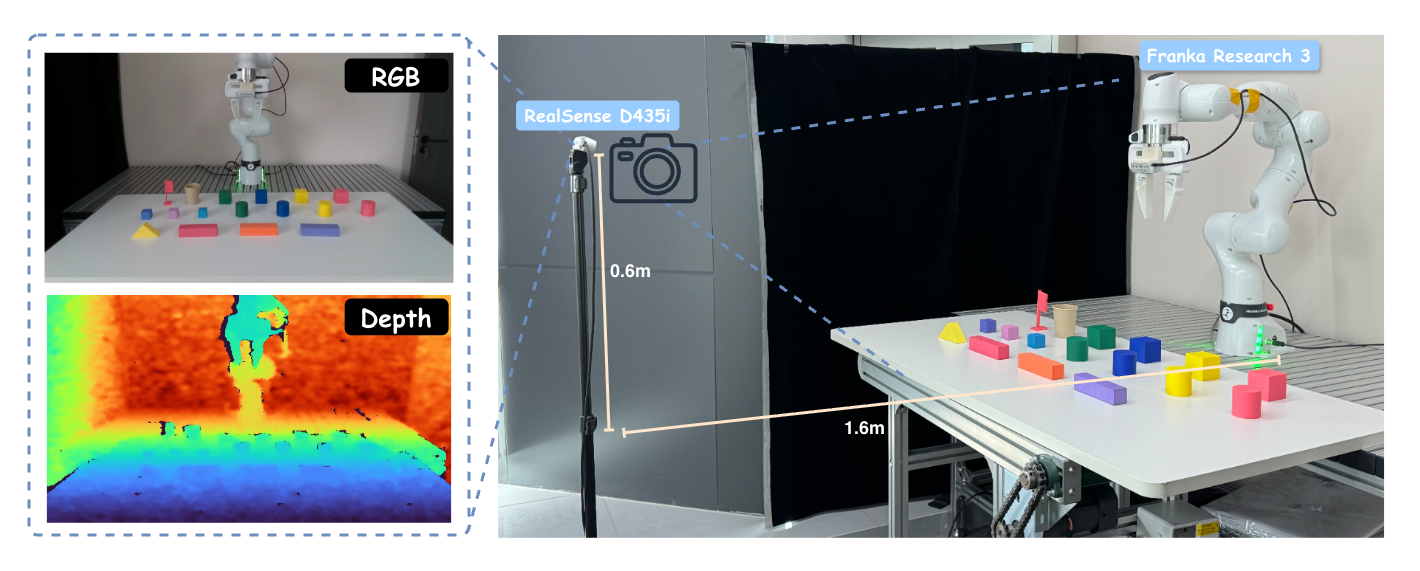
\includegraphics[width=0.72\textwidth]{Figures/appendix_robotenv.png}}%
    \begin{subfigure}[b]{0.25\textwidth}
        \centering
        \includegraphics[height=\robotheight]{Figures/appendix_franka.pdf}
        \caption{Franka Research 3.}
        \label{fig:appendix_franka}
    \end{subfigure}
    \hfill
    \begin{subfigure}[b]{0.72\textwidth}
        \centering
        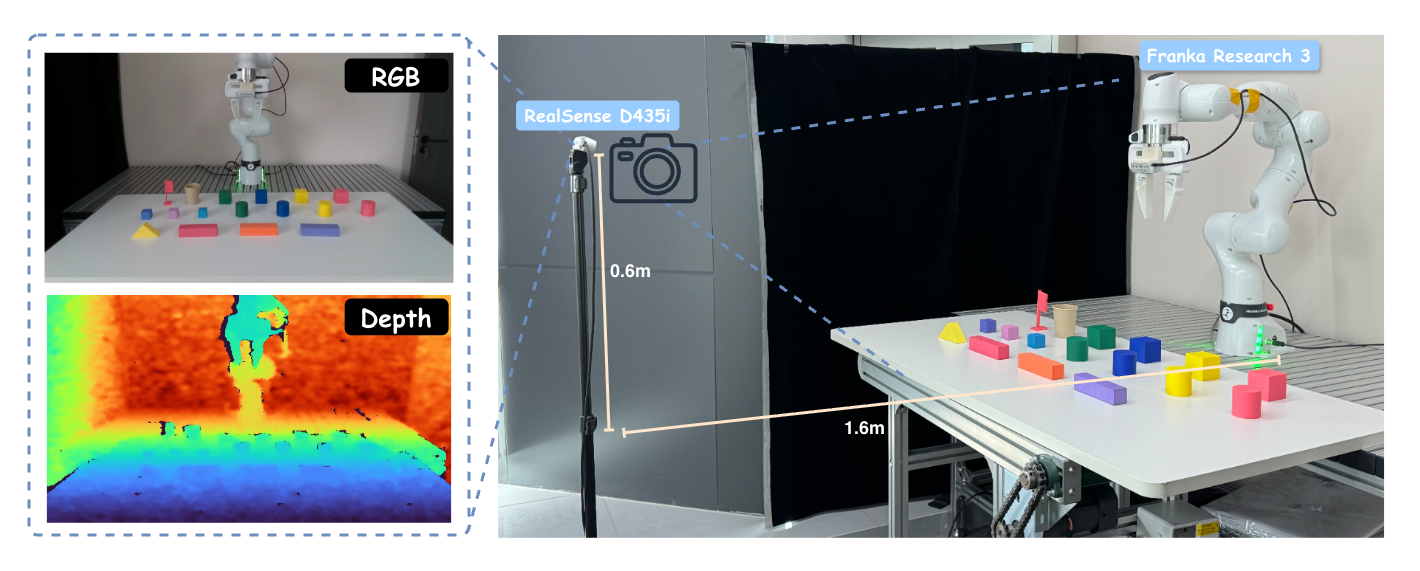
\includegraphics[width=\textwidth]{Figures/appendix_robotenv.png}
        \caption{Workspace setup with RGB and depth views.}
        \label{fig:appendix_robotenv}
    \end{subfigure}
    \caption{\textbf{Real-world experimental setup.} (a) The Franka Research 3 robot arm used in our experiments. (b) The physical workspace equipped with the robot arm and an Intel RealSense D435i camera; the insets show the corresponding RGB view and depth map.}
    \label{fig:appendix_robot_setup}
\end{figure}
\subsection{Experimental Assets and Task Design}
\noindent\textbf{Real-World Experimental Assets.} 
As shown in Fig.~\ref{fig:appendix_assets}, our real-world experiments utilize a diverse set of manipulation objects designed to evaluate precise spatial reasoning and sequential stacking. These assets primarily consist of: 
(i) \textit{Geometric primitives} including rectangular blocks, cubes, and cylinders in various sizes and distinct colors (pink, blue, green, yellow, purple, and orange); 
(ii) \textit{A triangular prism} (yellow triangle in Fig.~\ref{fig:appendix_assets}) used for assessing high-precision alignment and challenging placement tasks; and 
(iii) \textit{Functional objects} (e.g., a pink flag and a brown cup) to create dynamic occlusion and nesting scenarios. 
In total, these 17 unique pieces allow for a vast combinatorial space of long-horizon tasks, such as multi-layer block building and disassembling, providing a rigorous testbed for the model's object permanence and spatial consistency.

\begin{figure}[htbp]
    \centering
    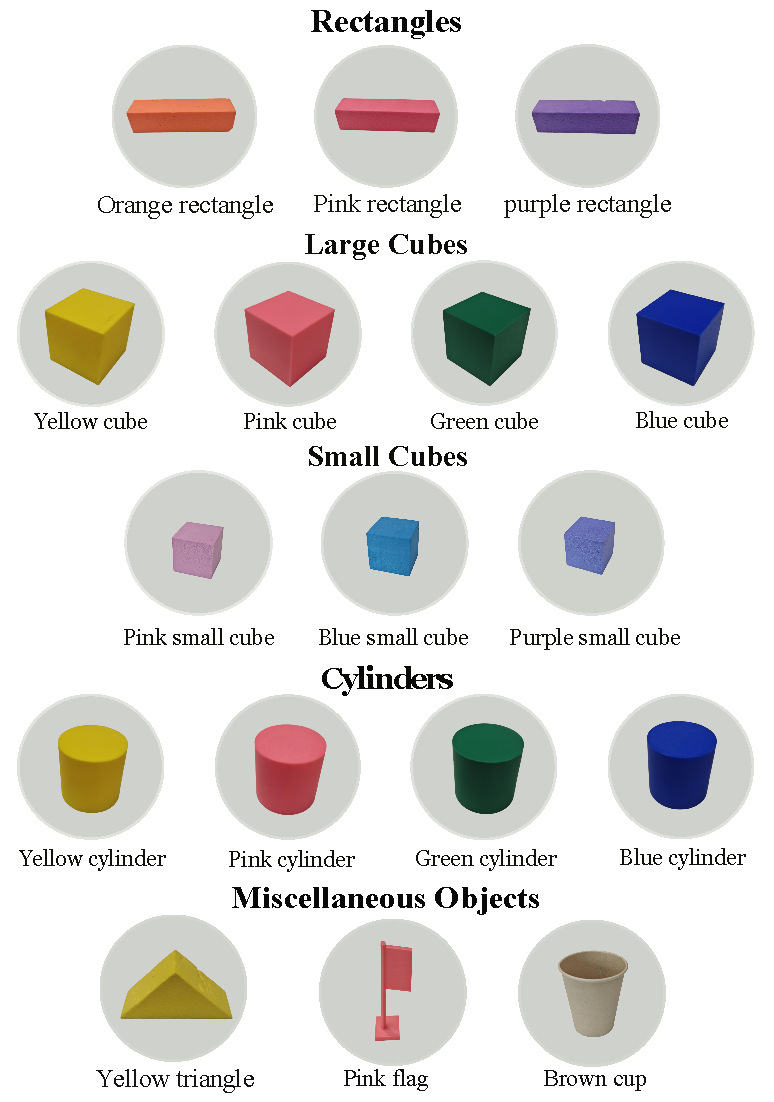
\includegraphics[width=0.6\textwidth]{Figures/appendix_assets.pdf} 
    \caption{\textbf{Assets for real-world experiments.} A collection of 17 manipulation objects including geometric primitives, a triangular prism, and functional objects used across all task difficulty levels.}
    \label{fig:appendix_assets}
\end{figure}

\subsubsection{Design of Real World Tasks}

Building on the experimental setup described in Sec.~\ref{sec:real_world}, we detail the task design across three difficulty levels. All tasks use the same Franka FR3 platform and RGB-D sensing described above.

\begin{itemize}
    \item \textbf{Easy \& Medium (Fig.~\ref{fig:appendix_step1}, \ref{fig:appendix_step2}):} Easy tasks involve 2--3 objects with single-step pick-and-place actions. Medium tasks extend to 4 objects and 3--4 sequential steps, requiring strict execution order. Both levels evaluate basic visual-language grounding and spatial precision.
    
    \item \textbf{Hard Block Building \& Disassembly (Fig.~\ref{fig:appendix_step3}):} These tasks involve up to 7 objects and 6--7 sequential actions. Building follows a Bottom-to-Top layer order for structural stability, while disassembly requires Top-to-Bottom single-anchor chaining to prevent collapse. These configurations test the model's understanding of physical support relationships over extended horizons.
    
    \item \textbf{Memorize \& Restore under Occlusion (Fig.~\ref{fig:appendix_step4}):} The robot hides an object (e.g., covering a cube with a cup), executes intermediate distractor actions, and must later recall the hidden object's location to restore the original scene. This directly evaluates causal memory retention and object permanence under occlusion---capabilities that purely reactive visual systems lack.
\end{itemize}

% --- Figures Below ---

\begin{figure}[htbp]
    \centering
    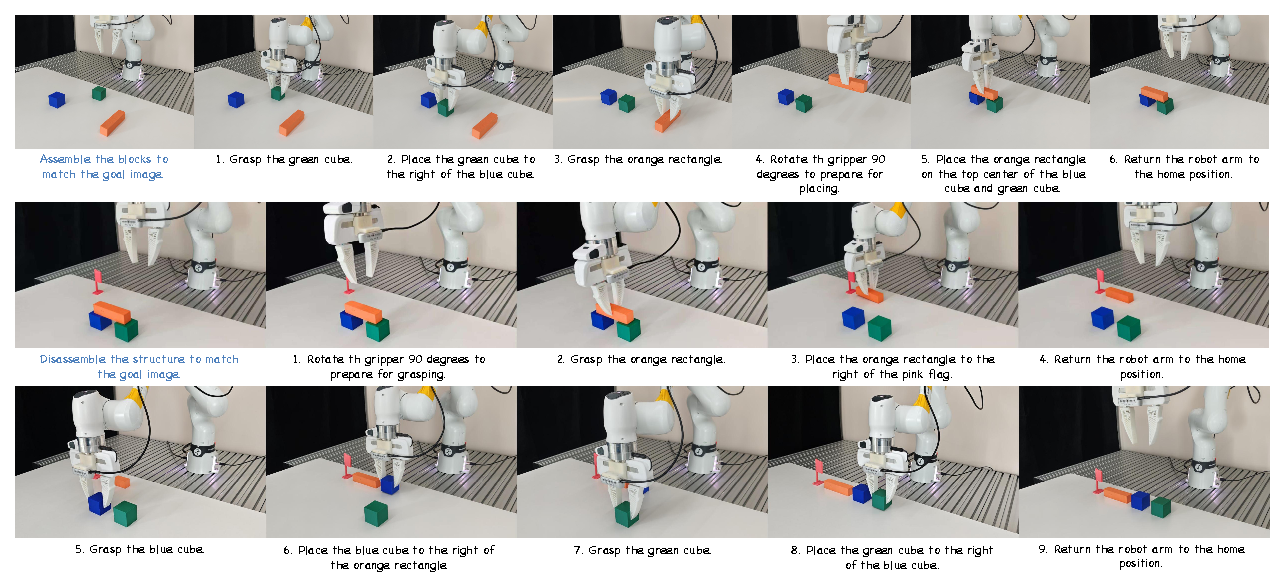
\includegraphics[width=1\textwidth]{Figures/appendix_realworld1.pdf} 
    \caption{\textbf{Multi-step block manipulation (Easy).} Execution of basic assembly and disassembly involving 2--3 objects, demonstrating fundamental spatial grounding and pick-and-place precision.}
    \label{fig:appendix_step1}
\end{figure}

\begin{figure}[htbp]
    \centering
    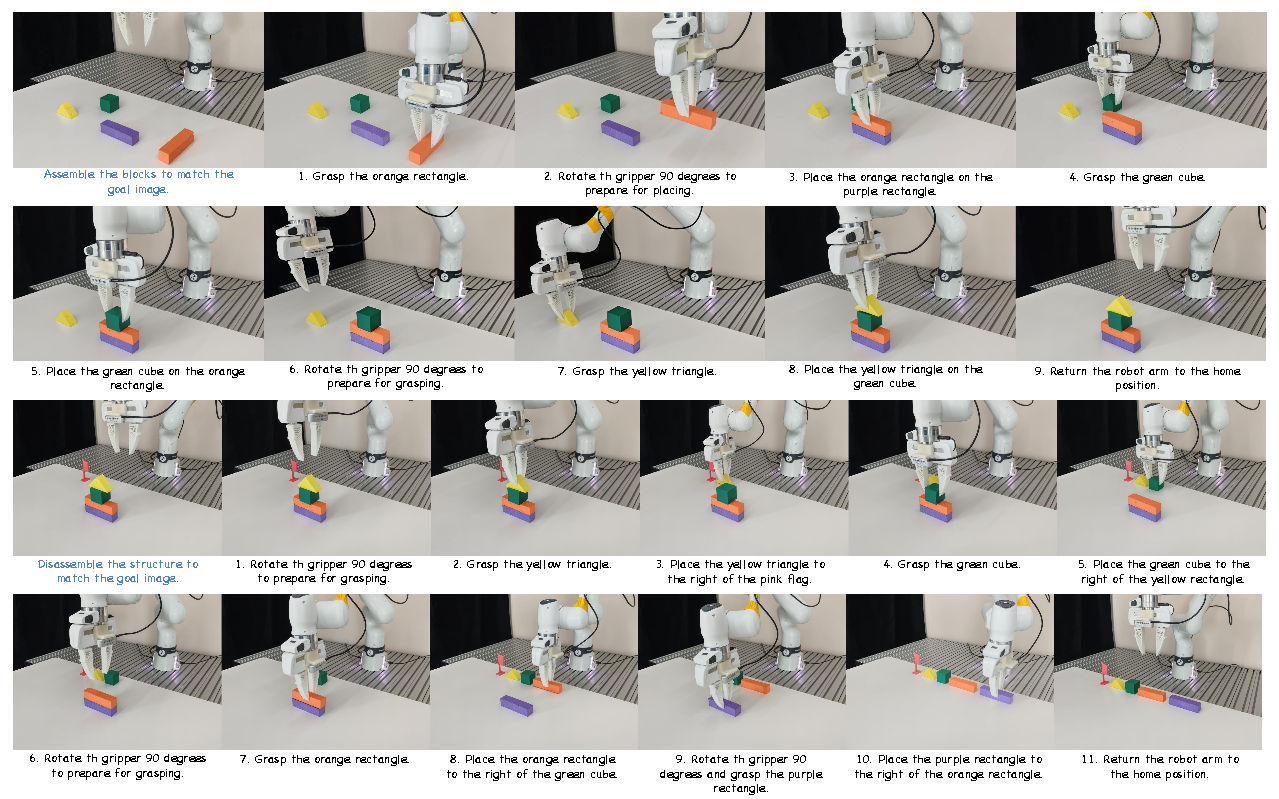
\includegraphics[width=1\textwidth]{Figures/appendix_realworld2.pdf} 
    \caption{\textbf{Multi-step block manipulation (Medium).} Intermediate execution requiring a strict sequence of 3--4 steps to manipulate 4 objects, verifying short-horizon sequential planning.}
    \label{fig:appendix_step2}
\end{figure}

\begin{figure}[htbp]
    \centering
    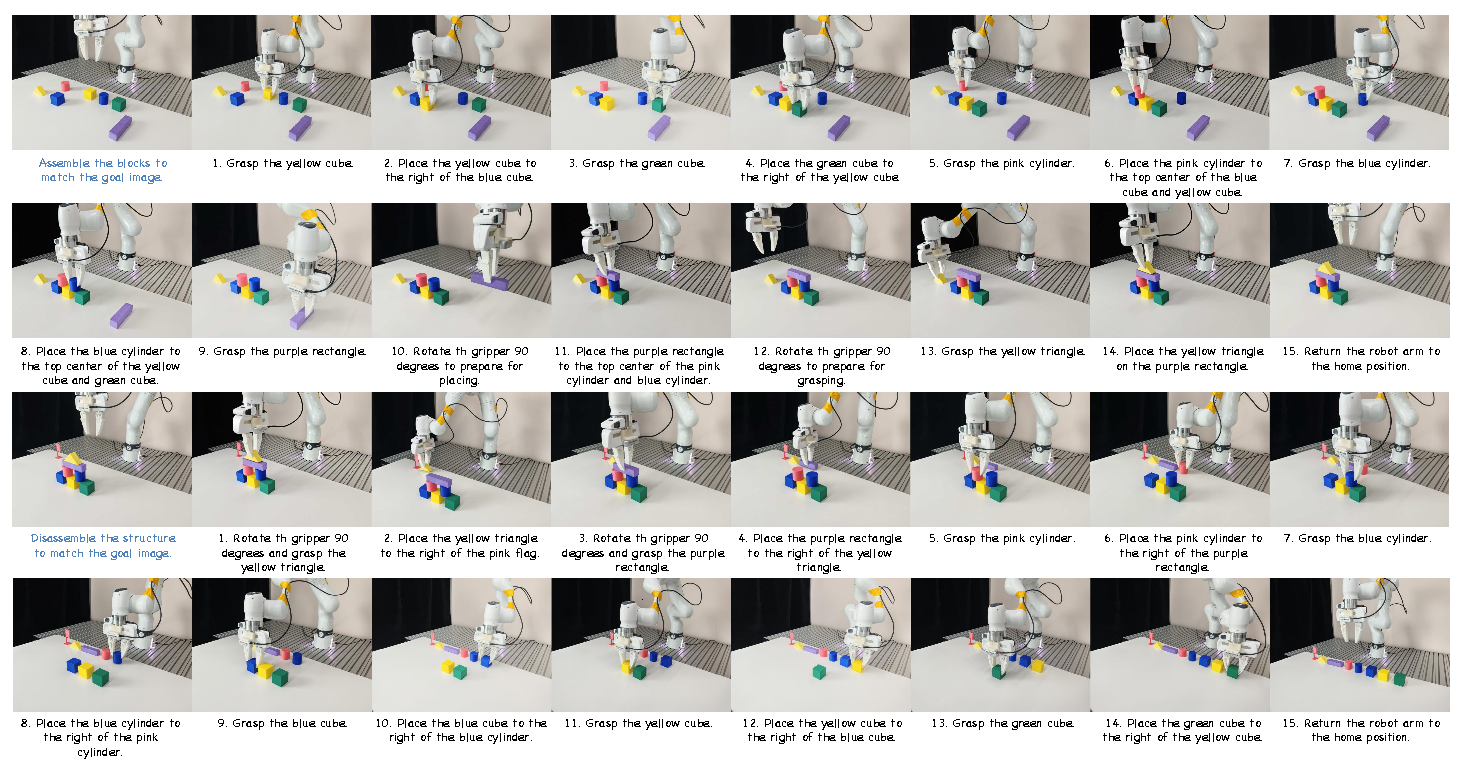
\includegraphics[width=1\textwidth]{Figures/appendix_realworld3.pdf} 
    \caption{\textbf{Multi-step block manipulation (Hard).} Extreme long-horizon execution involving 7 objects and 6--7 steps. The sequence highlights the model's ability to maintain physical stability during complex ``Bottom-to-Top'' building and ``Top-to-Bottom'' disassembly without collapsing the structure.}
    \label{fig:appendix_step3}
\end{figure}

\begin{figure}[htbp]
    \centering
    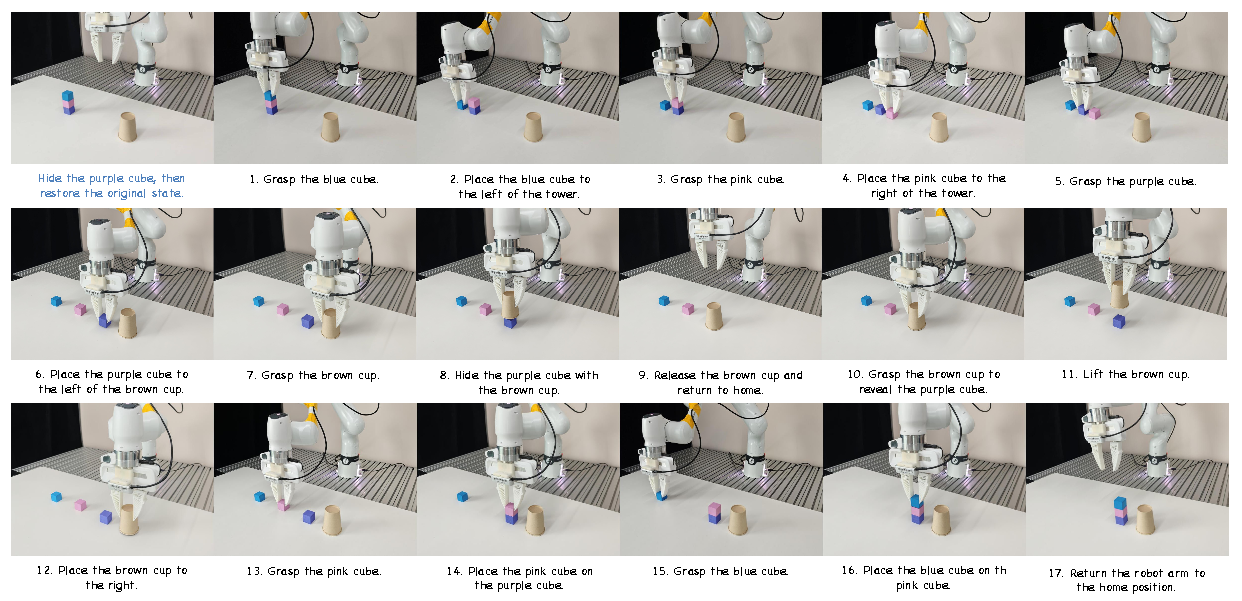
\includegraphics[width=1\textwidth]{Figures/appendix_realworld4.pdf} 
    \caption{\textbf{Long-horizon memorize and restore task (Occlusion).} A stress-test for causal memory retention. The robot sequentially hides the purple cube with a brown cup, performs intermediate tasks, and successfully recalls the hidden object's location to restore the original state.}
    \label{fig:appendix_step4}
\end{figure}


\subsubsection{Design of Simulation Tasks}
To comprehensively evaluate the capabilities of RoboStream, we carefully select and design tasks across two simulation platforms: SIMPLER~\cite{li2025evaluating} and RLBench~\cite{james2020rlbench}. Rather than treating all tasks uniformly, we deliberately categorize them into two distinct evaluation axes to independently stress-test zero-shot generalization, high-precision spatial grounding, and long-horizon causal memory.

\noindent\textbf{Evaluating Spatial Grounding and Zero-Shot Generalization.} 
The first suite of tasks is designed to isolate and evaluate the explicit 3D geometric grounding provided by STF-Tokens, independent of long-term memory requirements. To assess zero-shot cross-embodiment generalization, we deploy our framework in the SIMPLER benchmark (visualized in Fig.~\ref{fig:appendix_sim1}, top). We evaluate the Google Robot embodiment on tasks like ``Pick Coke Can'' and ``Move Near'', alongside the WidowX + Bridge embodiment on tasks such as ``Put Spoon on Towel'', ``Put Carrot on Plate'', ``Stack Green Block on Yellow Block'', and ``Put Eggplant in Basket''. The design rationale here is to verify that the spatio-temporal reasoning enabled by STF-Tokens is not overfitted to a specific robot kinematic structure or camera viewpoint. By deploying RoboStream on unseen embodiments without fine-tuning, we demonstrate its robustness to visual domain shifts and novel spatial layouts. 

Complementing this cross-embodiment evaluation, we select 15 diverse single-step tasks from the standard RLBench suite (e.g., \textit{Close Drawer, Lamp Off, Meat Off Grill, Put Rubbish in Bin, Slide Block to Target}, as shown in Fig.~\ref{fig:appendix_sim1}, bottom). The primary motivation for including these short-horizon tasks is their demand for fine-grained geometric understanding and contact-rich interactions. Testing on these specific scenarios allows us to prove that explicit 3D geometric representations—captured via centroids and Gaussian shapes—surpass pixel-level implicit reasoning even before complex sequential planning is required.

\noindent\textbf{Evaluating Causal Memory and Object Permanence.} 
To explicitly stress-test the Causal Spatio-Temporal Graph (CSTG) and its ability to maintain object permanence, we engineer a custom suite of 8 complex, long-horizon tasks in RLBench. These tasks are structured around two distinct guidance modalities to evaluate different aspects of persistent memory. The first category consists of goal-image guided tasks (\textit{Bridge Between Towers, Place Blocks in Two Containers (Normal/Hard), and Stack Three/Five Colors}, visualized in Fig.~\ref{fig:appendix_sim2}). In these scenarios, the robot must deduce the correct multi-step execution sequence from a visually complex target state. This design tests the model's capacity to maintain spatial coherence and track multiple object states simultaneously as the scene dynamically evolves. 

The second category introduces text-guided tasks (\textit{Cover Top/Bottom Block with Box, and Unstack then Stack Four Colors}, visualized in Fig.~\ref{fig:appendix_sim3}), which are specifically designed to evaluate causal memory under severe occlusion. By instructing the robot to hide a target object and subsequently restore the environment, we force the system to rely entirely on its episodic memory log rather than immediate visual perception. This task design acts as a rigorous stress test, proving the absolute necessity of the CSTG in preventing spatial hallucinations when visual evidence is temporarily lost.

\begin{figure}[htpb]
    \centering
    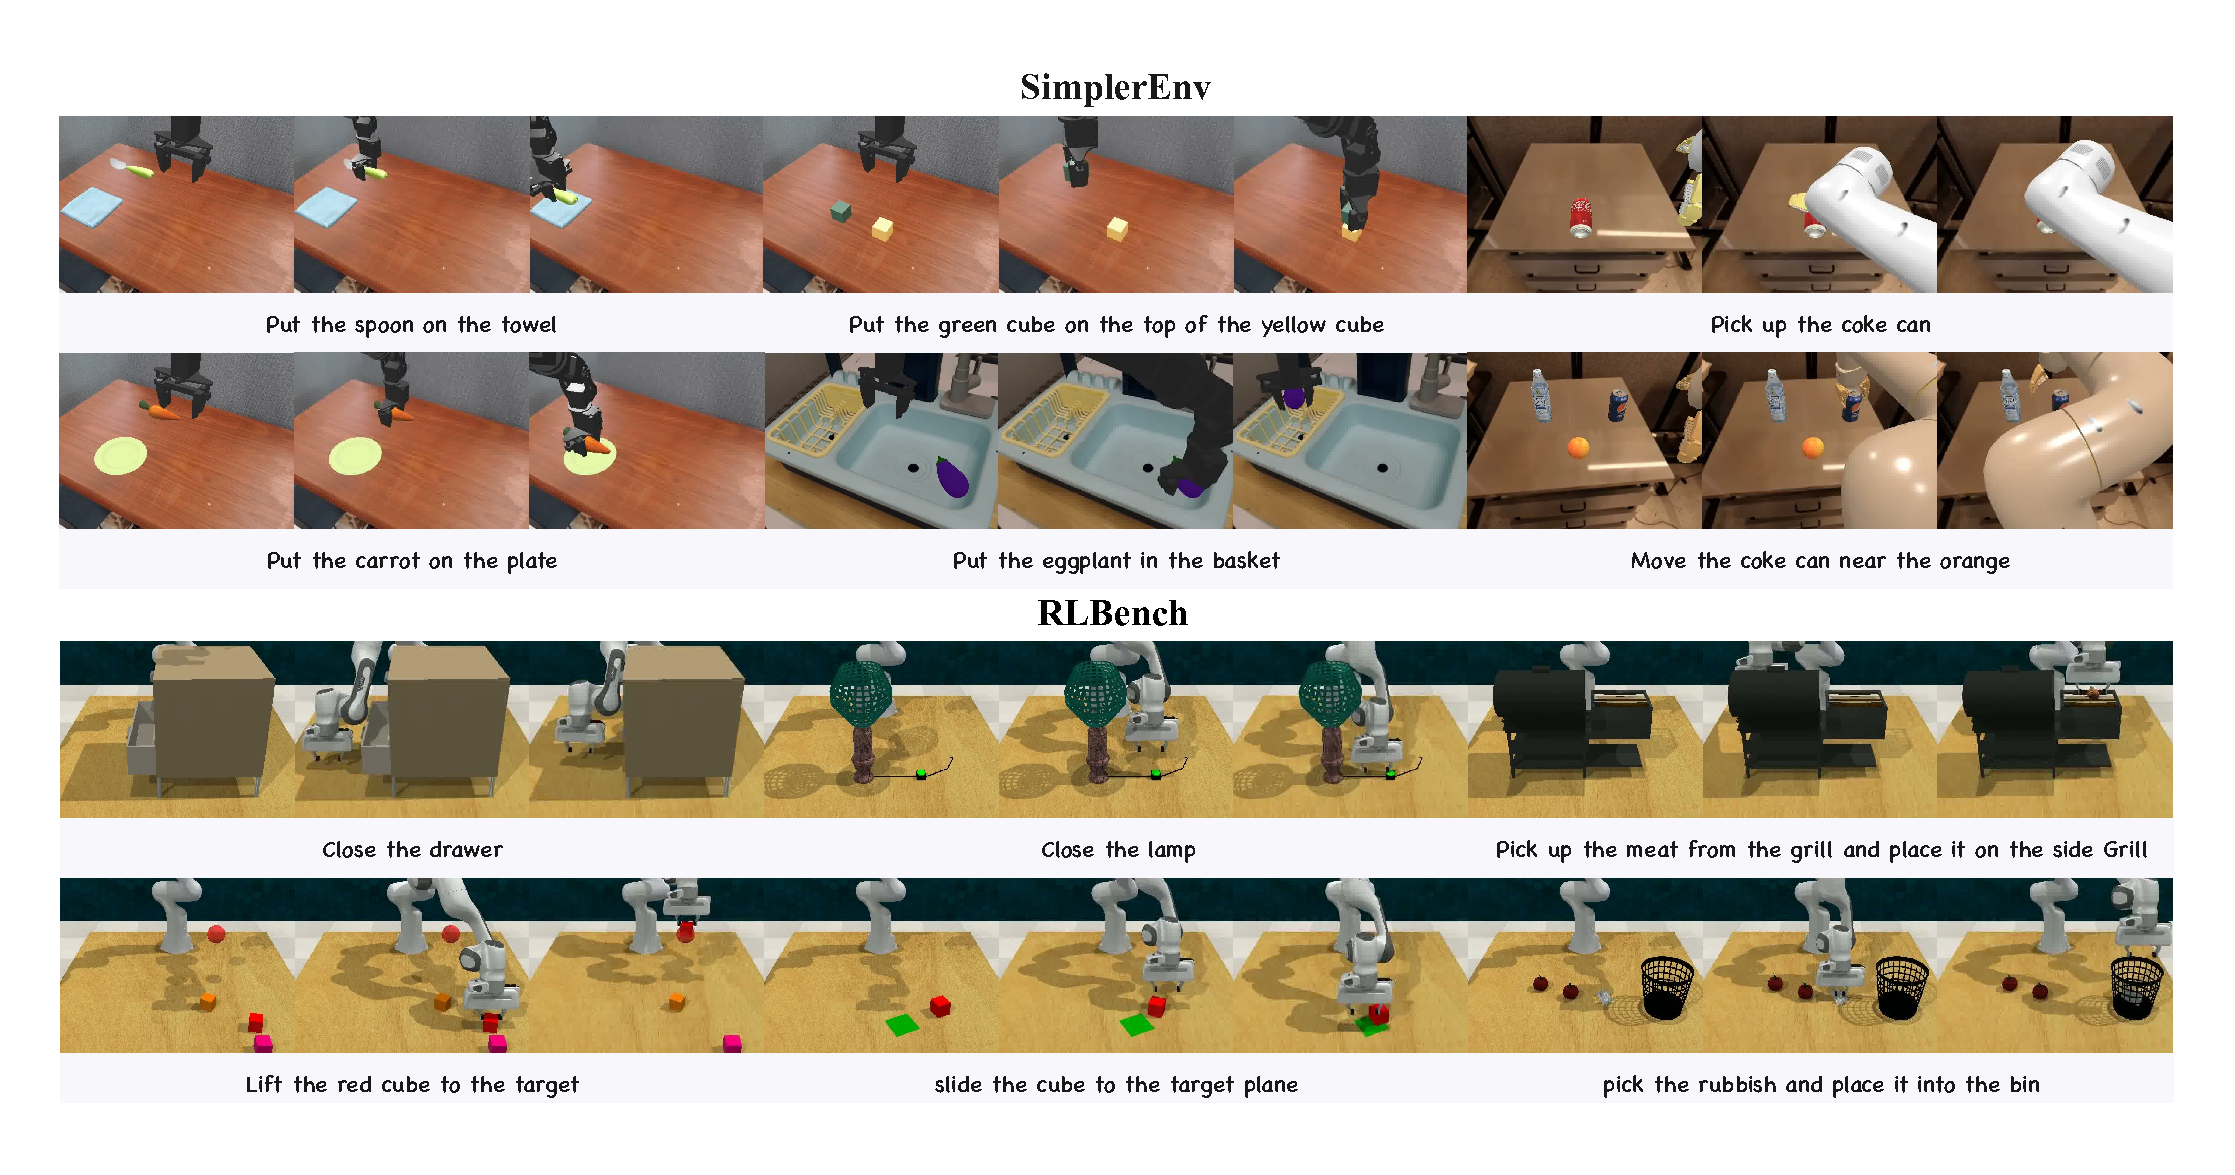
\includegraphics[width=1\textwidth]{Figures/RoboStream_Sim_OneStep.pdf} 
    \caption{\textbf{Visualization of Single-Step Evaluation Tasks.} Execution examples from the SIMPLER environment (top) and RLBench (bottom). These tasks are designed to demonstrate the model's zero-shot cross-embodiment generalization and its capability for high-precision spatial grounding in contact-rich scenarios.}
    \label{fig:appendix_sim1}
\end{figure}

\begin{figure}[htpb]
    \centering
    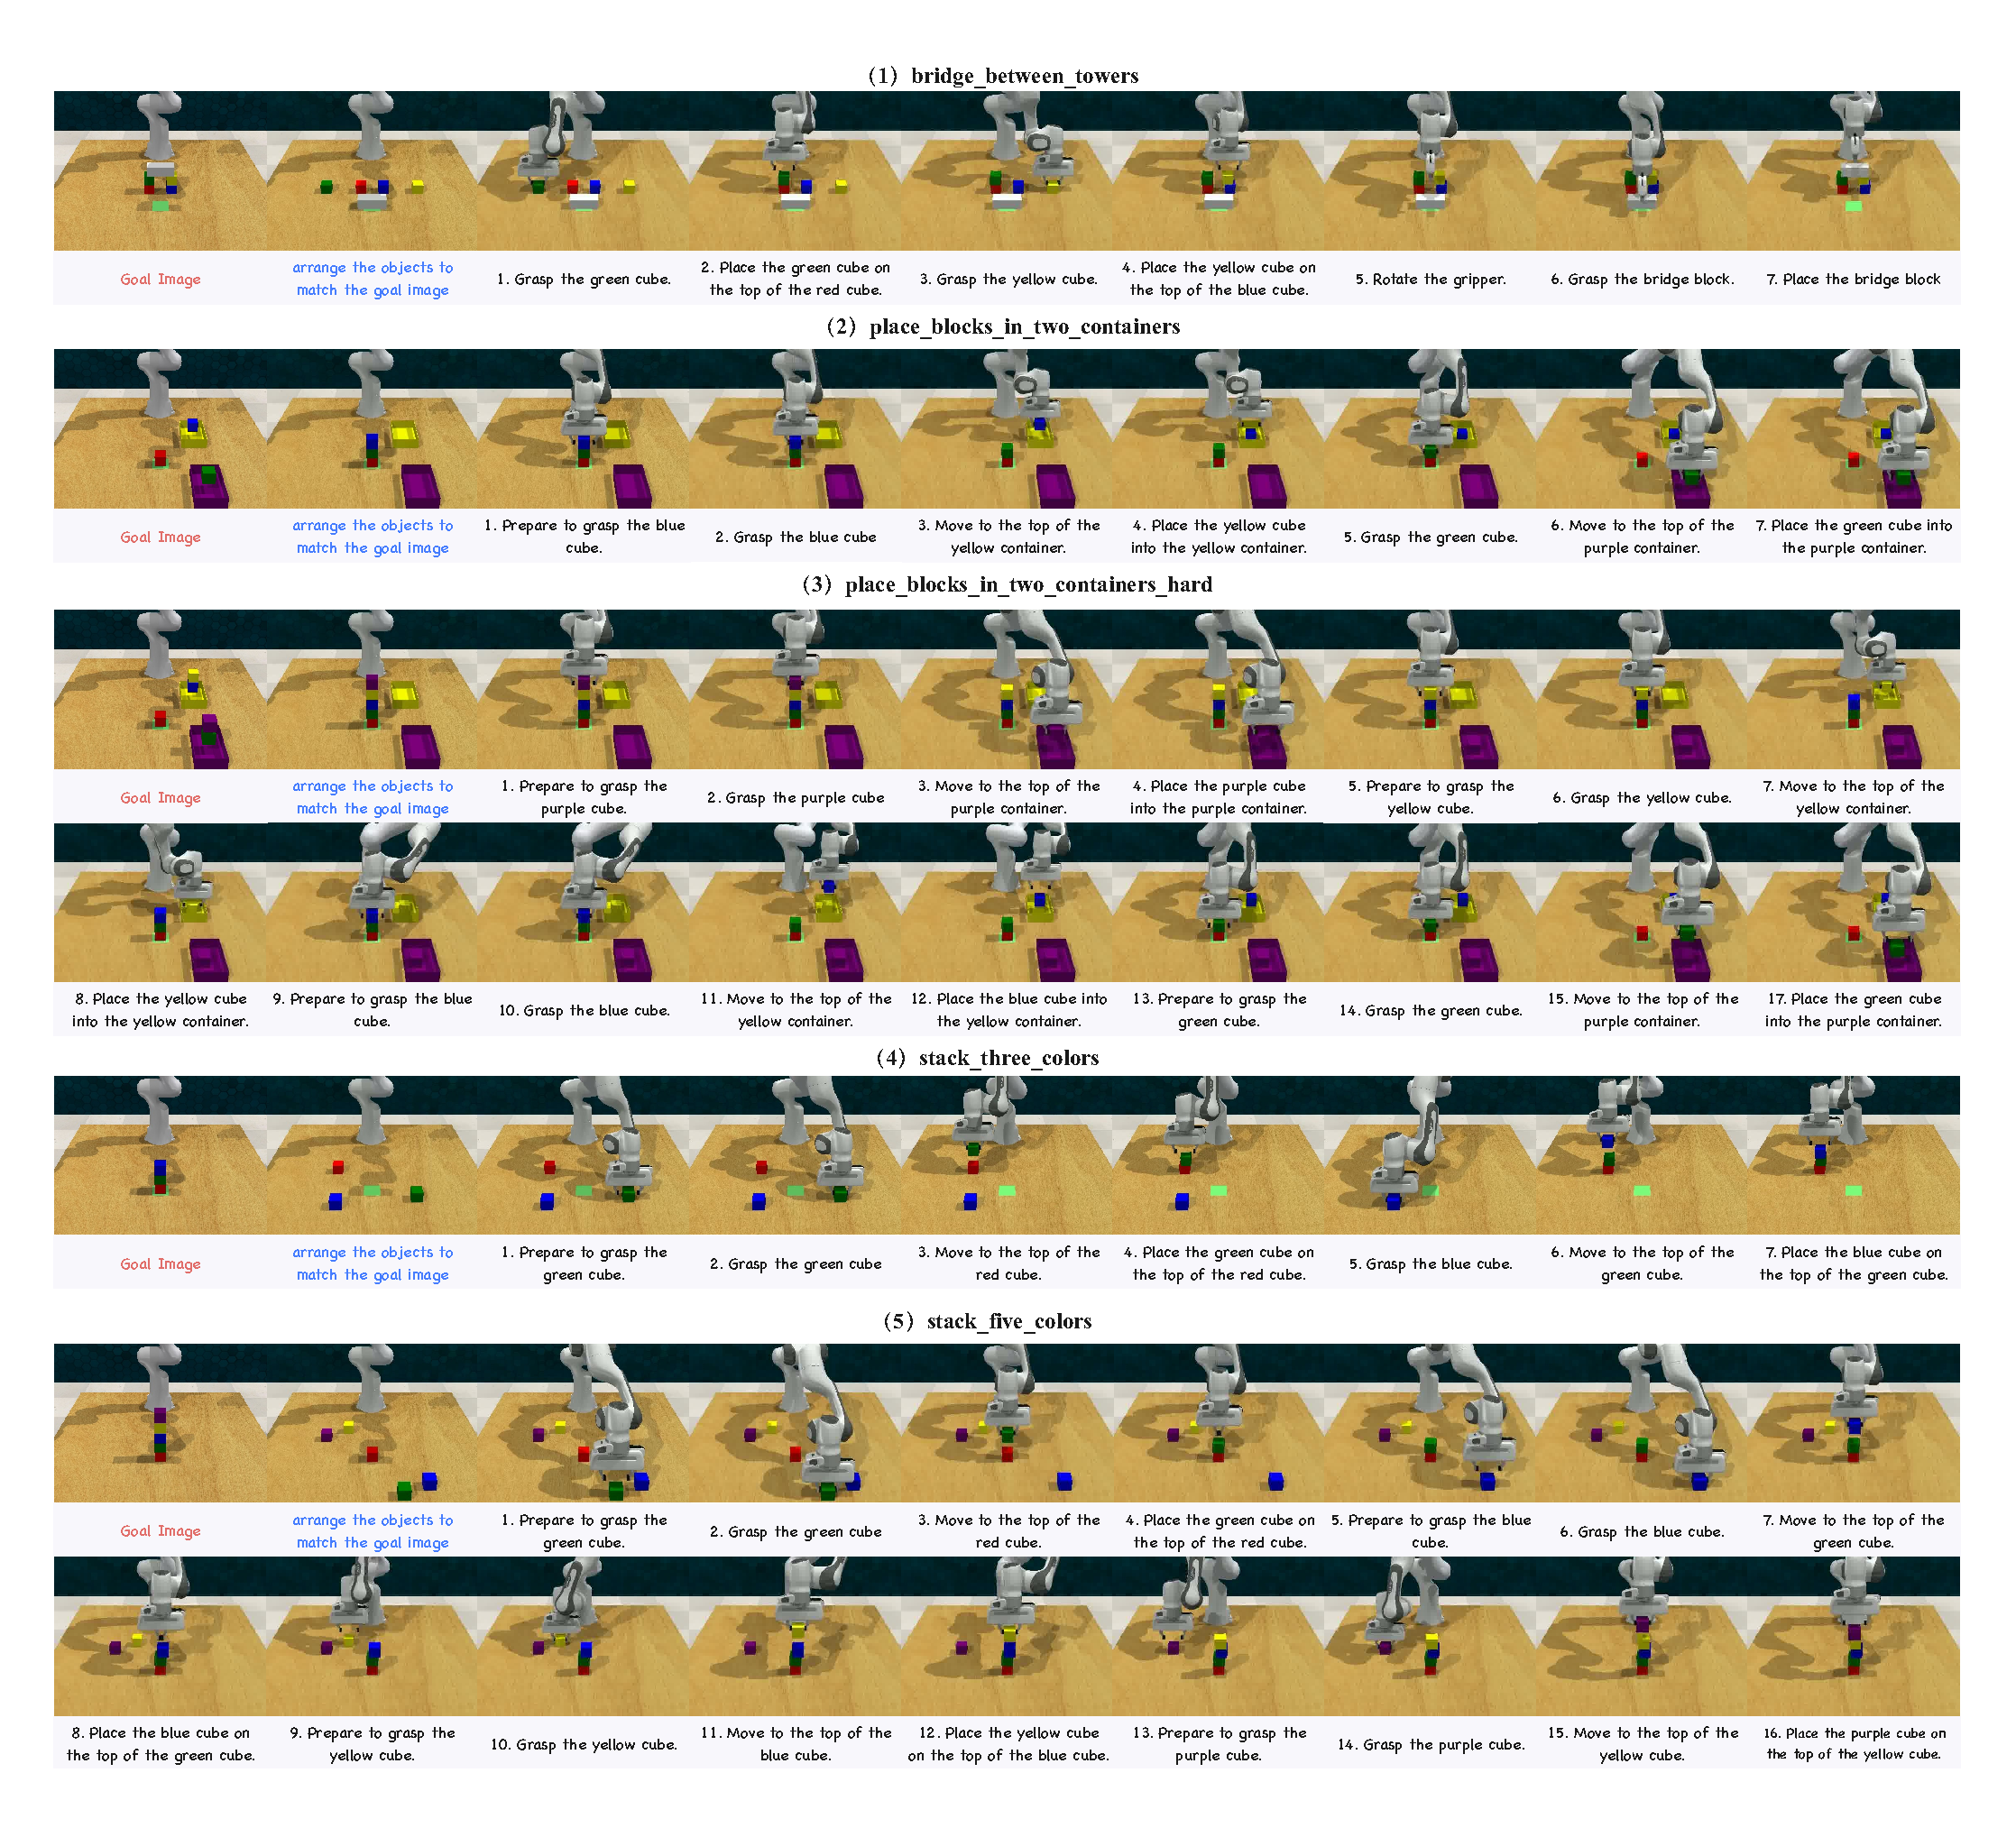
\includegraphics[width=1\textwidth]{Figures/RoboStream_MultiStep_Goal_Img.pdf} 
    \caption{\textbf{Goal-Image Guided Multi-Step Tasks.} Execution sequences for five long-horizon tasks in RLBench where the target state is provided via a visual goal image. These tasks systematically evaluate the model's ability to maintain spatial coherence and track multiple objects across extended dynamic trajectories.}
    \label{fig:appendix_sim2}
\end{figure}

\begin{figure}[htpb]
    \centering
    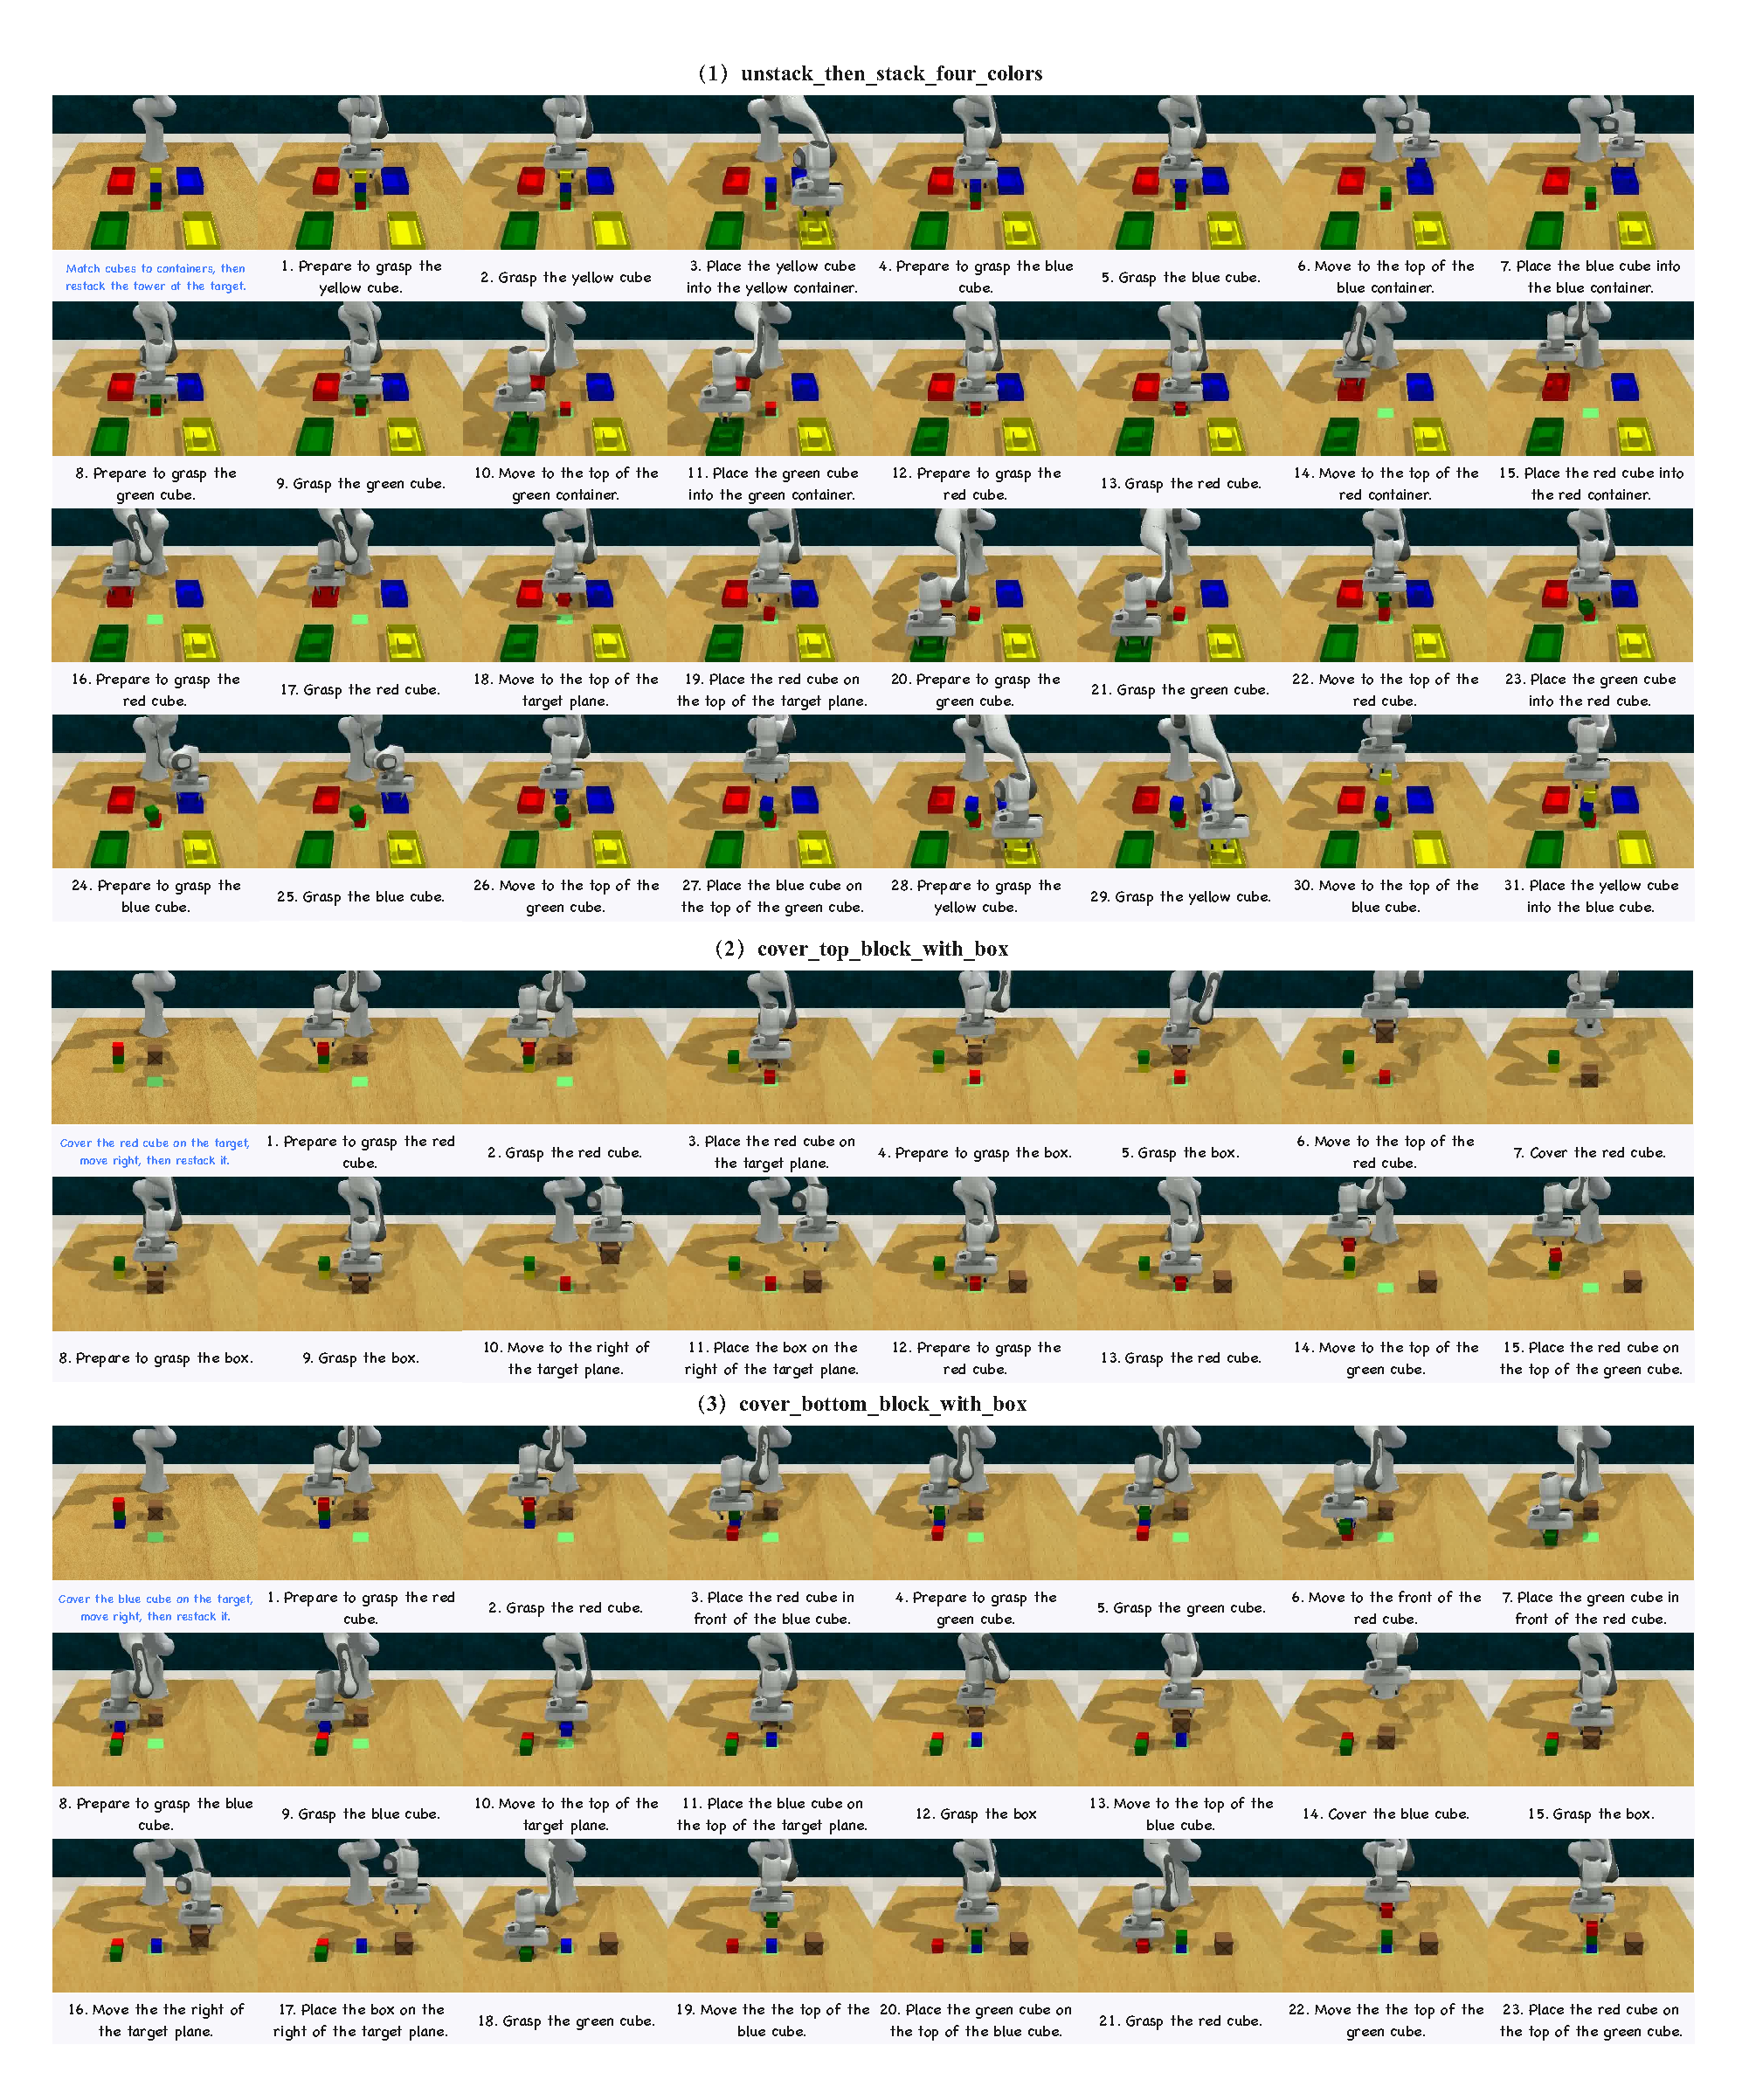
\includegraphics[width=1\textwidth]{Figures/RoboStream_MultiStep_Text.pdf} 
    \caption{\textbf{Text-Guided Multi-Step Tasks.} Execution sequences for three complex long-horizon tasks in RLBench driven by natural language instructions. Notably, tasks involving covering and revealing blocks rigorously stress-test the Causal Spatio-Temporal Graph (CSTG) for object permanence and causal memory retention under severe occlusion.}
    \label{fig:appendix_sim3}
\end{figure}

\subsection{Detailed Experimental Results}
\subsubsection{Detailed Results of Real-World Manipulation}
\begin{table}[htbp]
    \centering
    % \caption{\textbf{Detailed quantitative results of real-world tasks.} For Block Building and Disassembly, the \textit{Task} column shows the \textbf{goal state} to be achieved. For the Memorize \& Restore task, it instead shows the \textbf{initial scene state} paired with a text instruction, since the objective is to restore the scene after a hidden manipulation sequence.}
    \caption{\textbf{Detailed quantitative results of real-world tasks.}}
    \label{tab:real_world_detailed}
    \renewcommand{\arraystretch}{1.1} 
    \resizebox{\textwidth}{!}{
    \begin{tabular}{m{0.3\textwidth} c c c c c c}
        \toprule
        % 使用 multirow 和 multicolumn 将“任务属性”和“模型成功率”在视觉上彻底分开
        \multirow{2}{*}{\textbf{Task}} & \multirow{2}{*}{\textbf{Difficulty}} & \multicolumn{5}{c}{\textbf{Success Rate}} \\
        \cmidrule(lr){3-7}
        & & \textbf{SoFar} & \textbf{VoxPoser} & \textbf{RoboStream-8B} & \textbf{RoboStream-32B} & \textbf{RoboStream-235B} \\
        \midrule
        
        % ==================== Section 1: 搭积木 ====================
        \multicolumn{7}{c}{\textit{Block Building (Bottom-to-Top)} {\scriptsize $\vert$ \textit{Task $=$ Goal Image}}} \\
        \midrule
        \begin{minipage}{0.3\textwidth}
            \centering \vspace{1pt}
            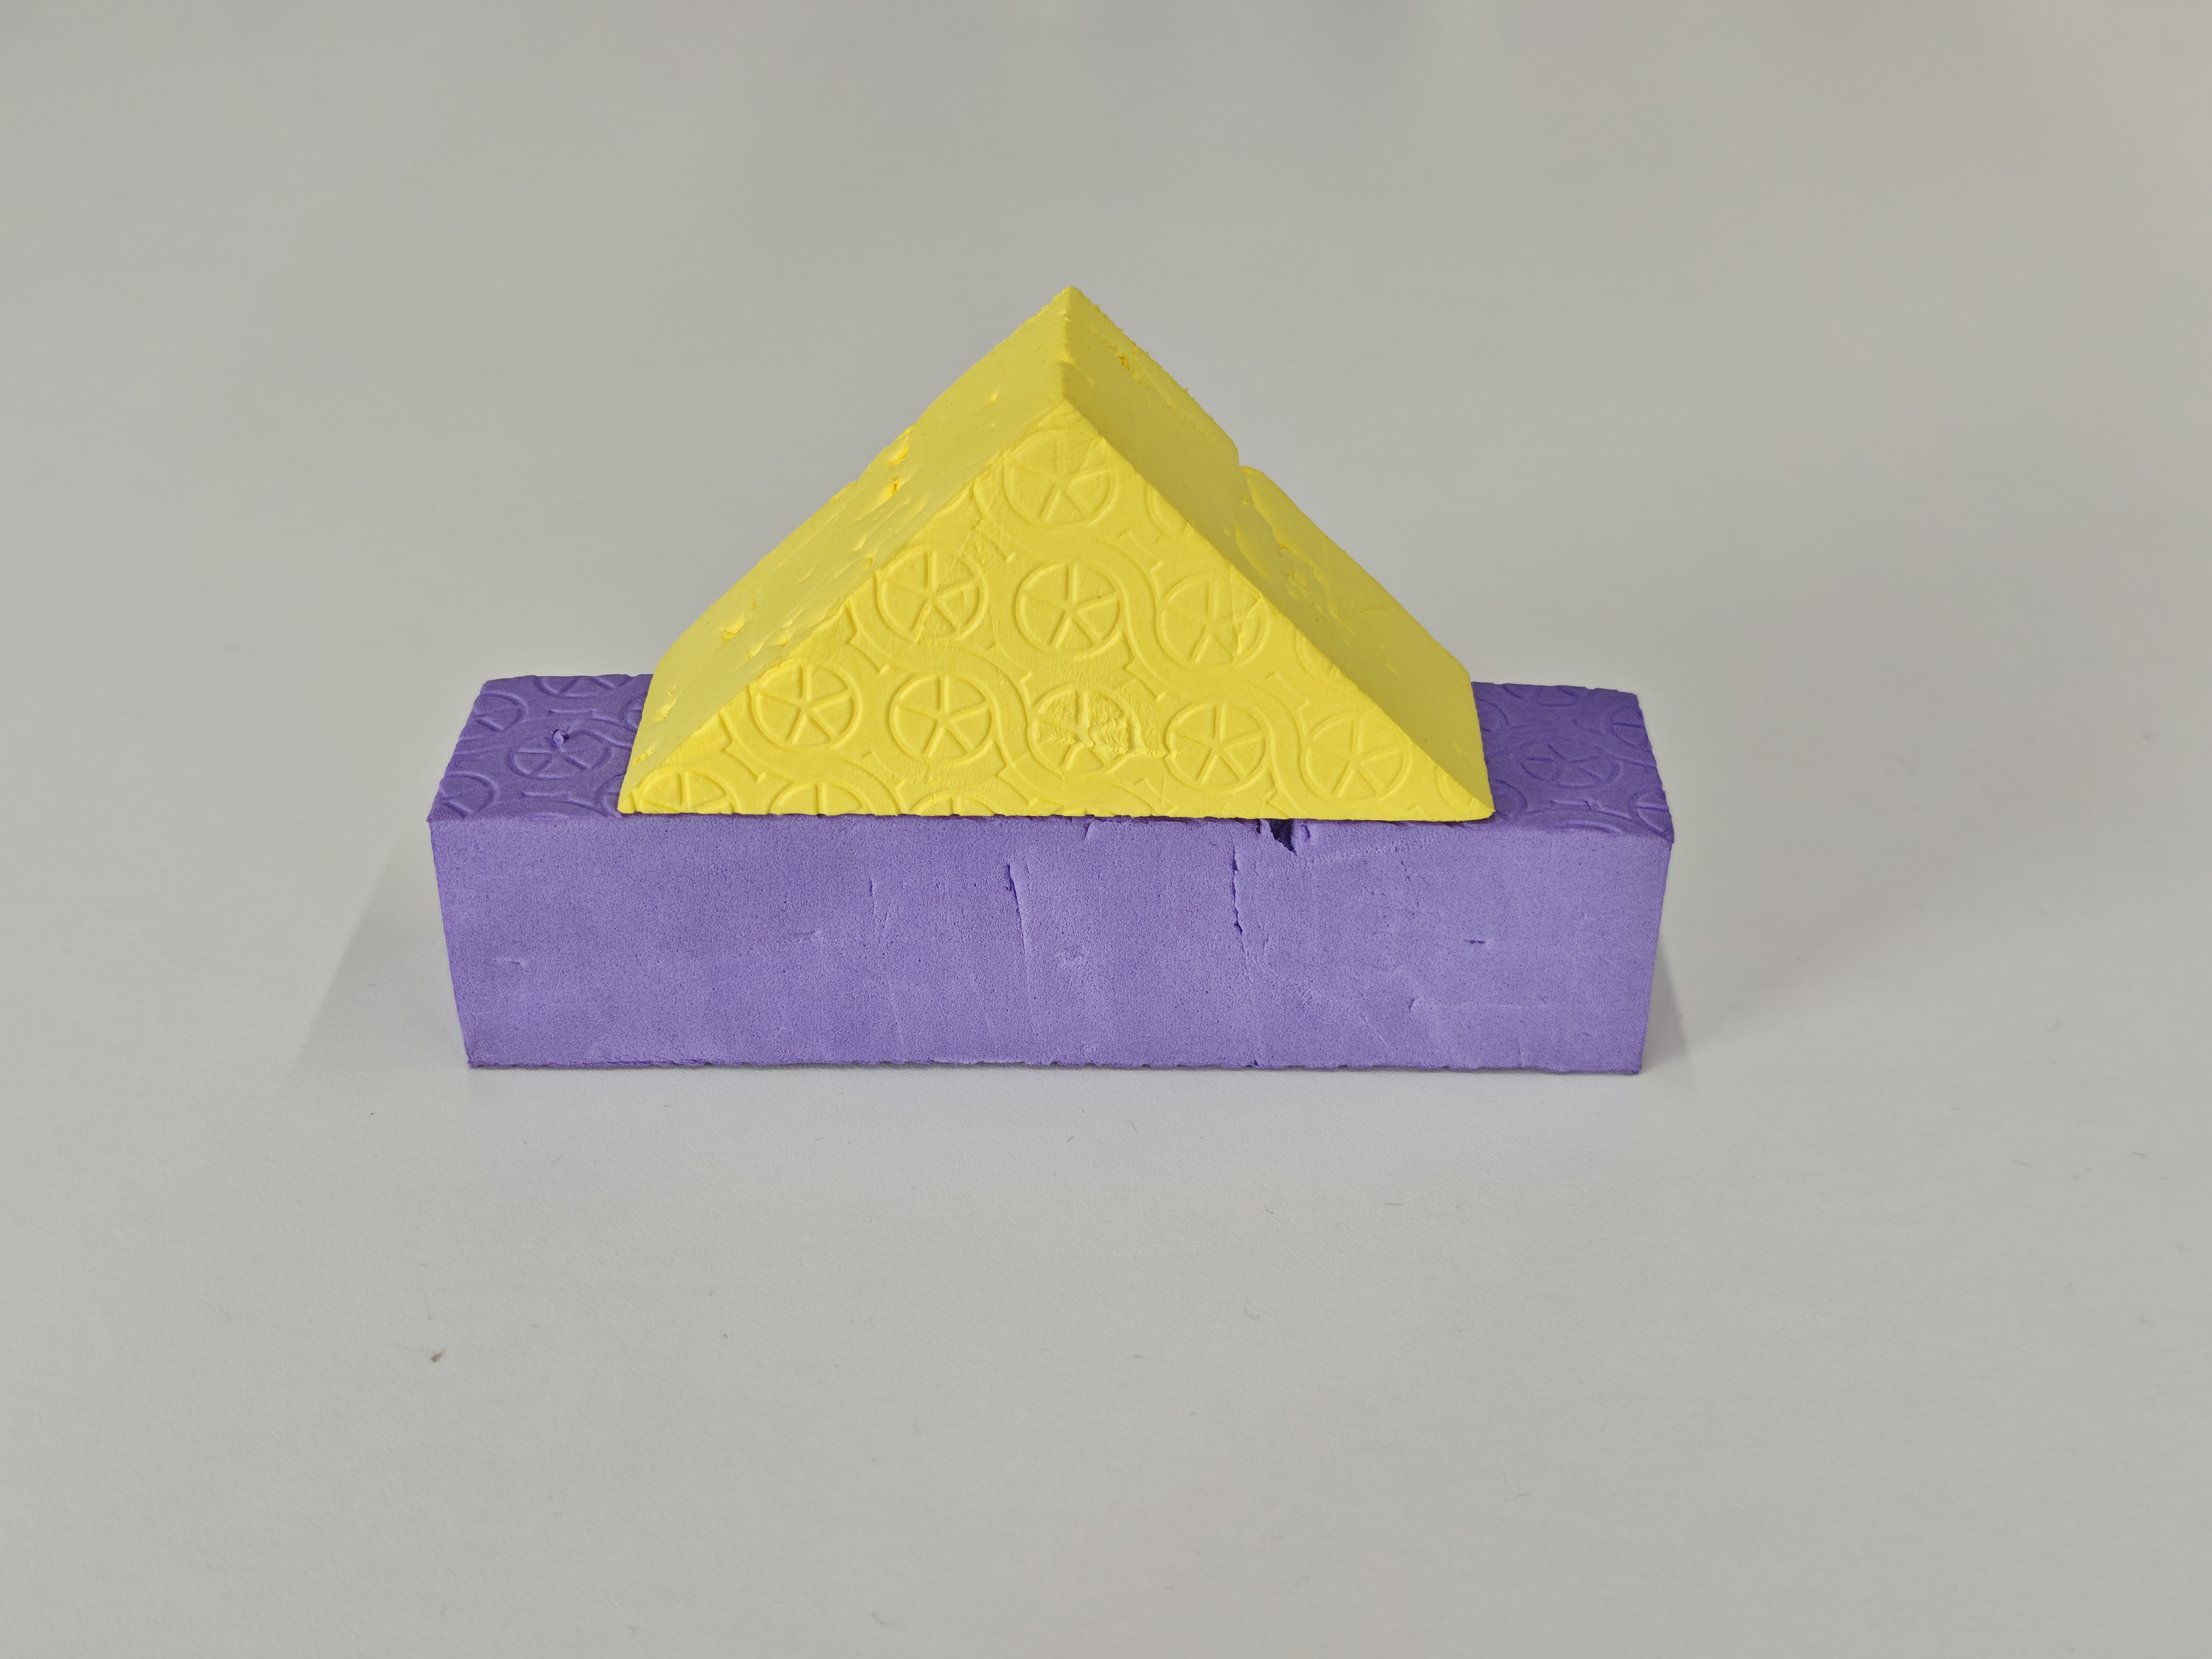
\includegraphics[height=1.0cm]{Figures/goal_images/easy1.jpg}
            \vspace{1pt}
        \end{minipage} 
        & Easy & 3/3 & 2/3 & 1/3 & 2/3 & \textbf{2/3} \\
        
        \begin{minipage}{0.3\textwidth}
            \centering \vspace{1pt}
            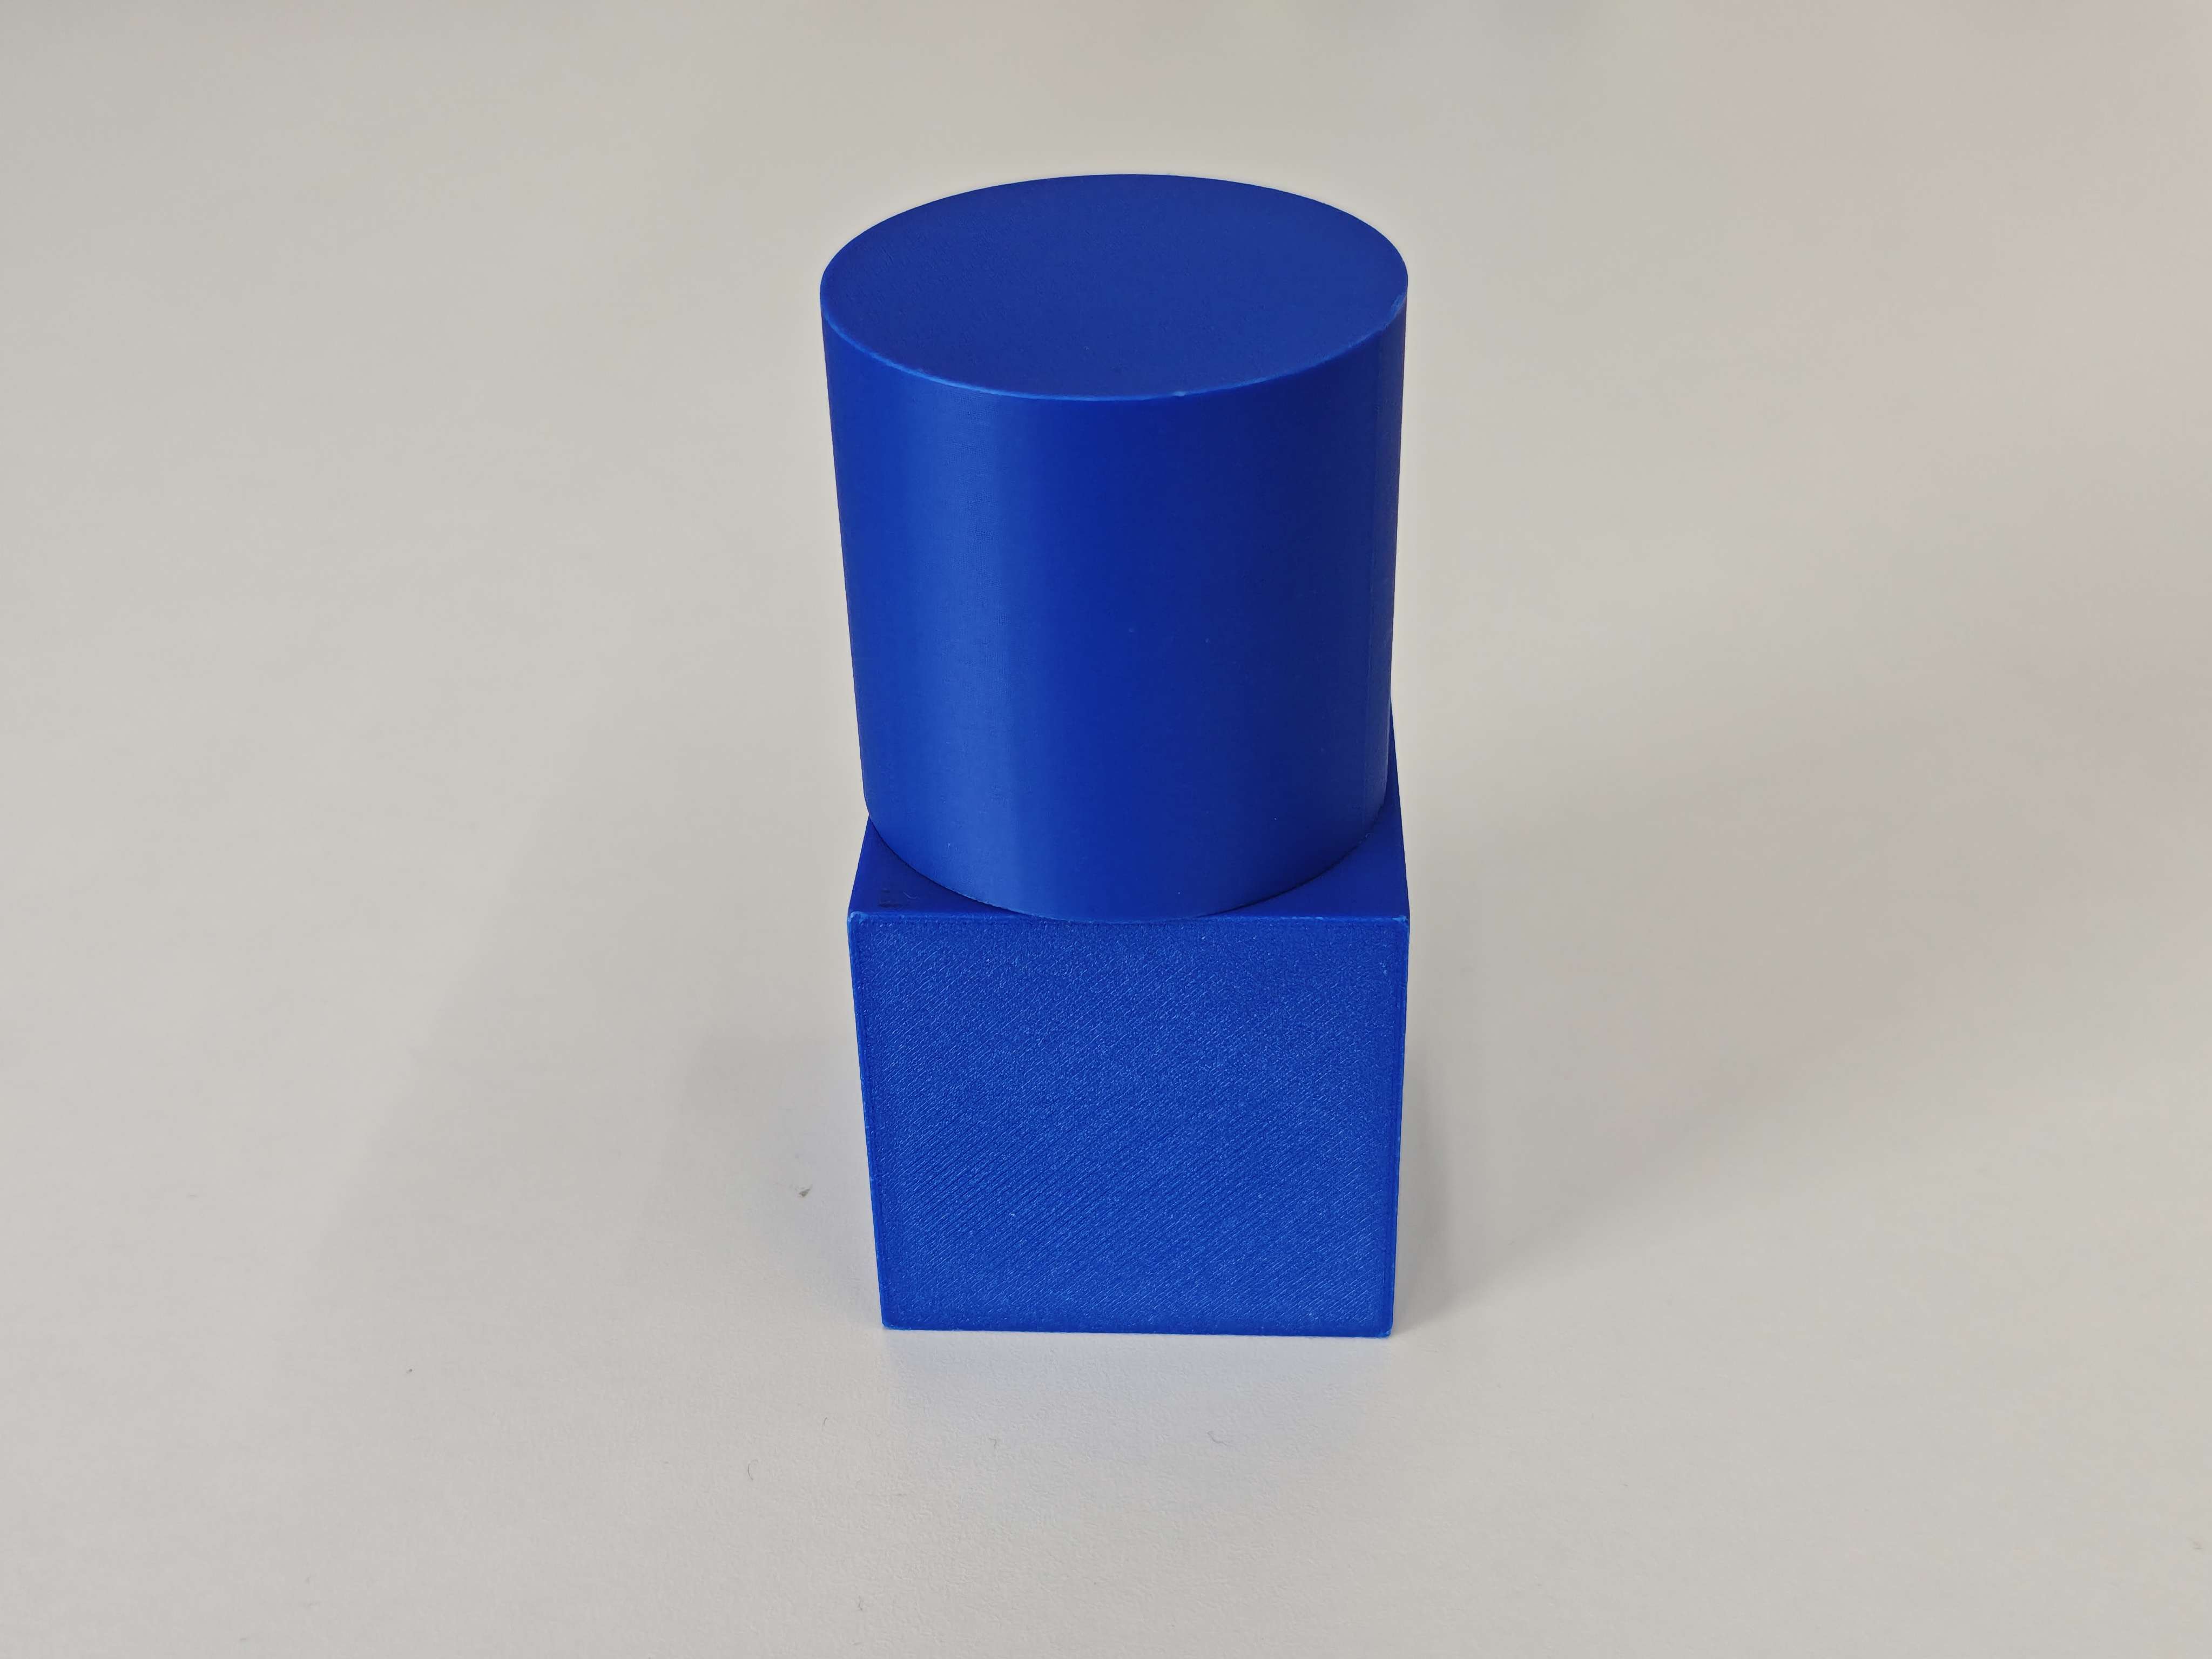
\includegraphics[height=1.0cm]{Figures/goal_images/easy2.jpg}
            \vspace{1pt}
        \end{minipage} 
        & Easy & 2/3 & 2/3 & 3/3 & 1/3 & \textbf{3/3} \\
        
        \begin{minipage}{0.3\textwidth}
            \centering \vspace{1pt}
            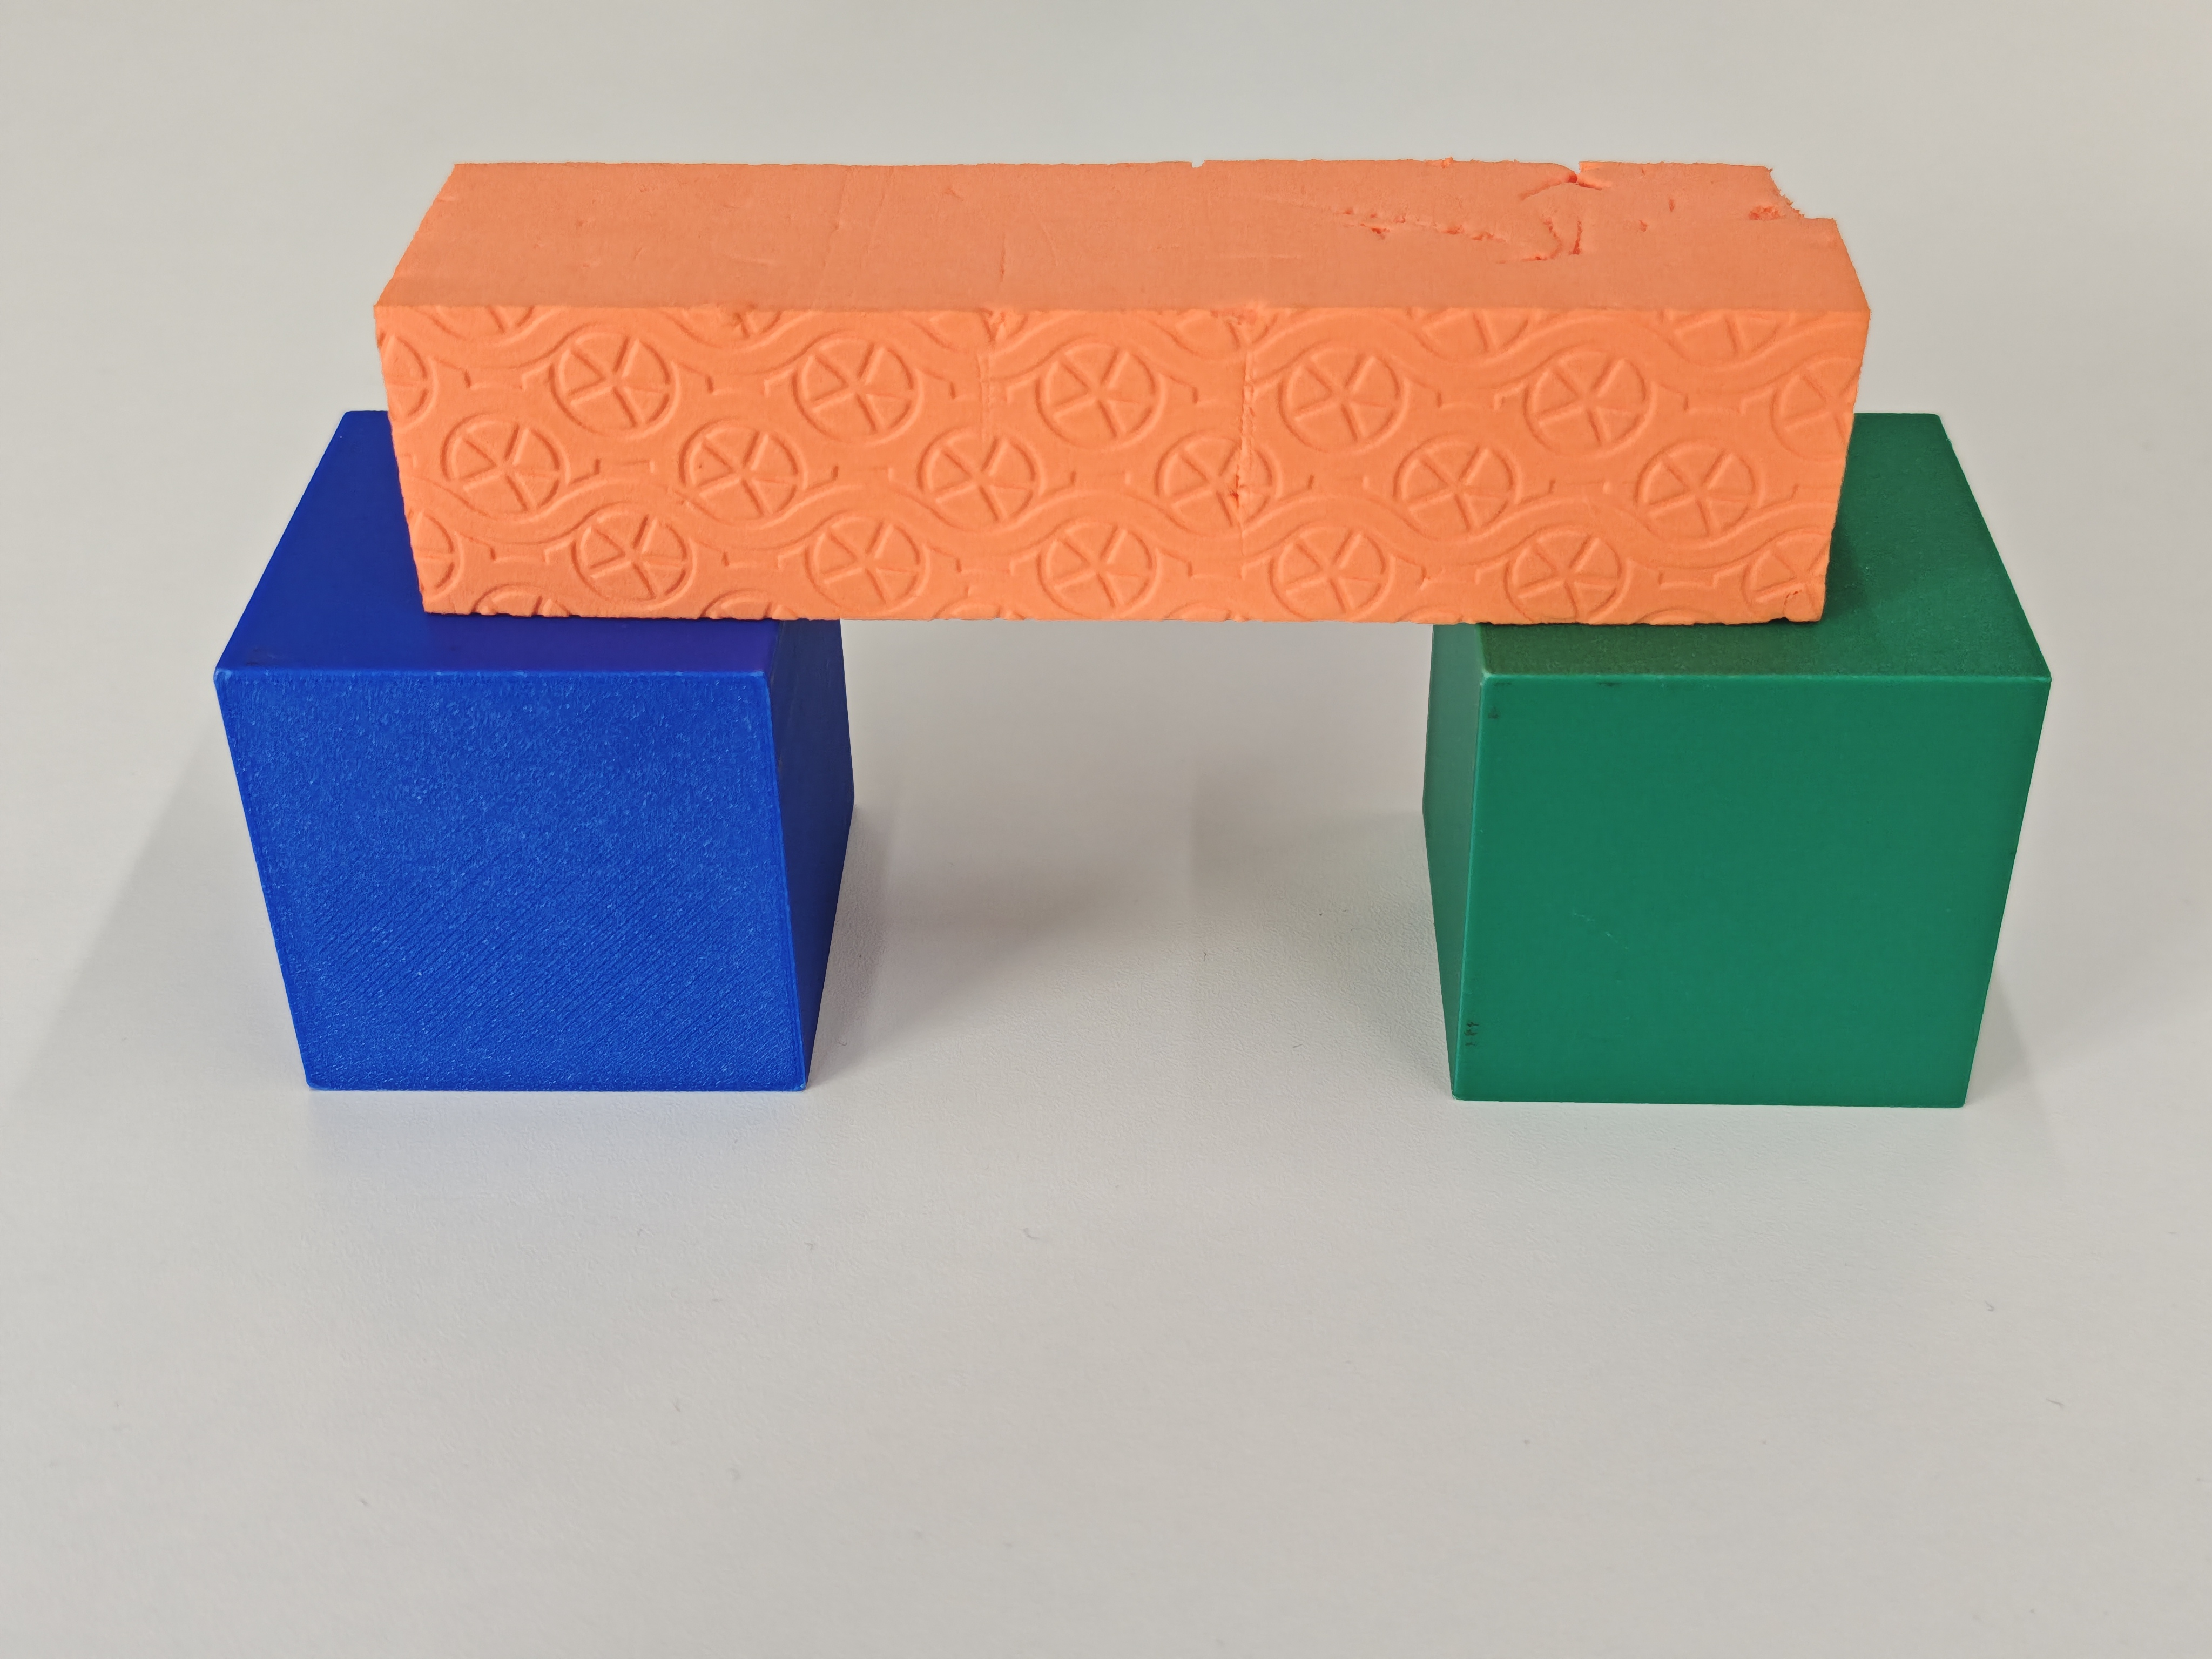
\includegraphics[height=1.0cm]{Figures/goal_images/easy3.jpg}
            \vspace{1pt}
        \end{minipage} 
        & Easy & 0/3 & 0/3 & 1/3 & 3/3 & \textbf{2/3} \\
        
        \begin{minipage}{0.3\textwidth}
            \centering \vspace{1pt}
            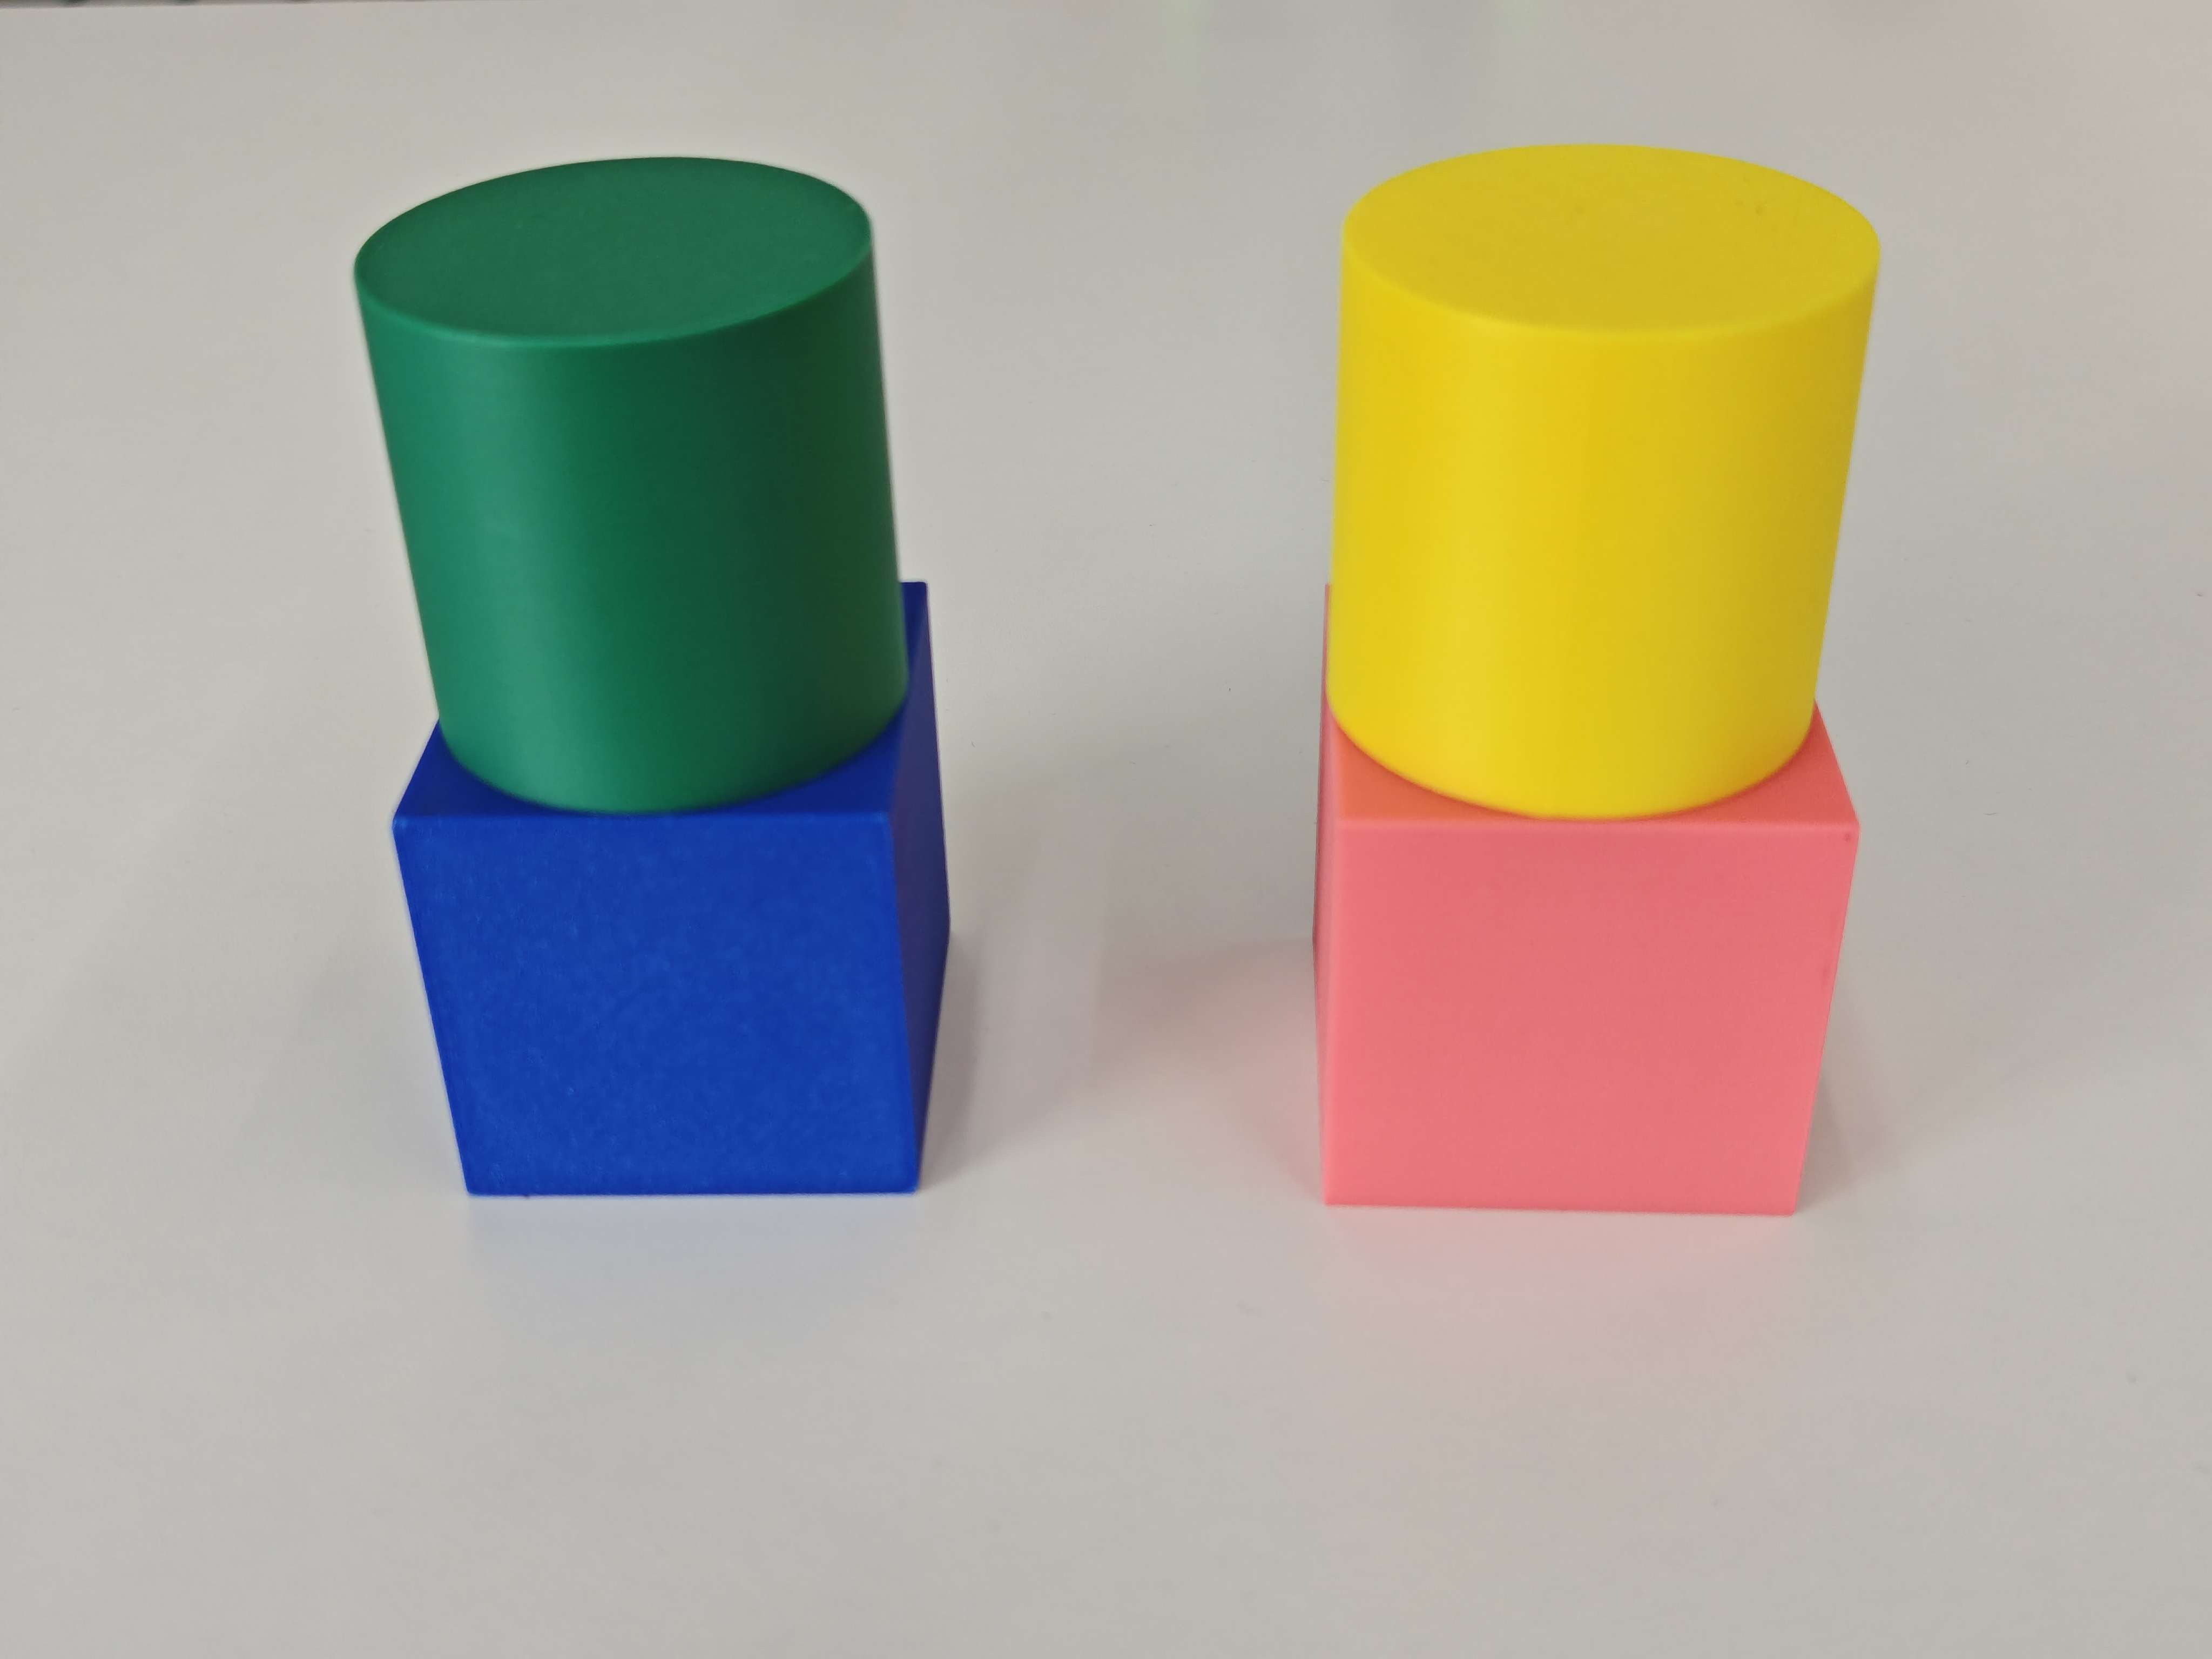
\includegraphics[height=1.0cm]{Figures/goal_images/medium1.jpg}
            \vspace{1pt}
        \end{minipage} 
        & Medium & 0/3 & 2/3 & 2/3 & 2/3 & \textbf{3/3} \\
        
        \begin{minipage}{0.3\textwidth}
            \centering \vspace{1pt}
            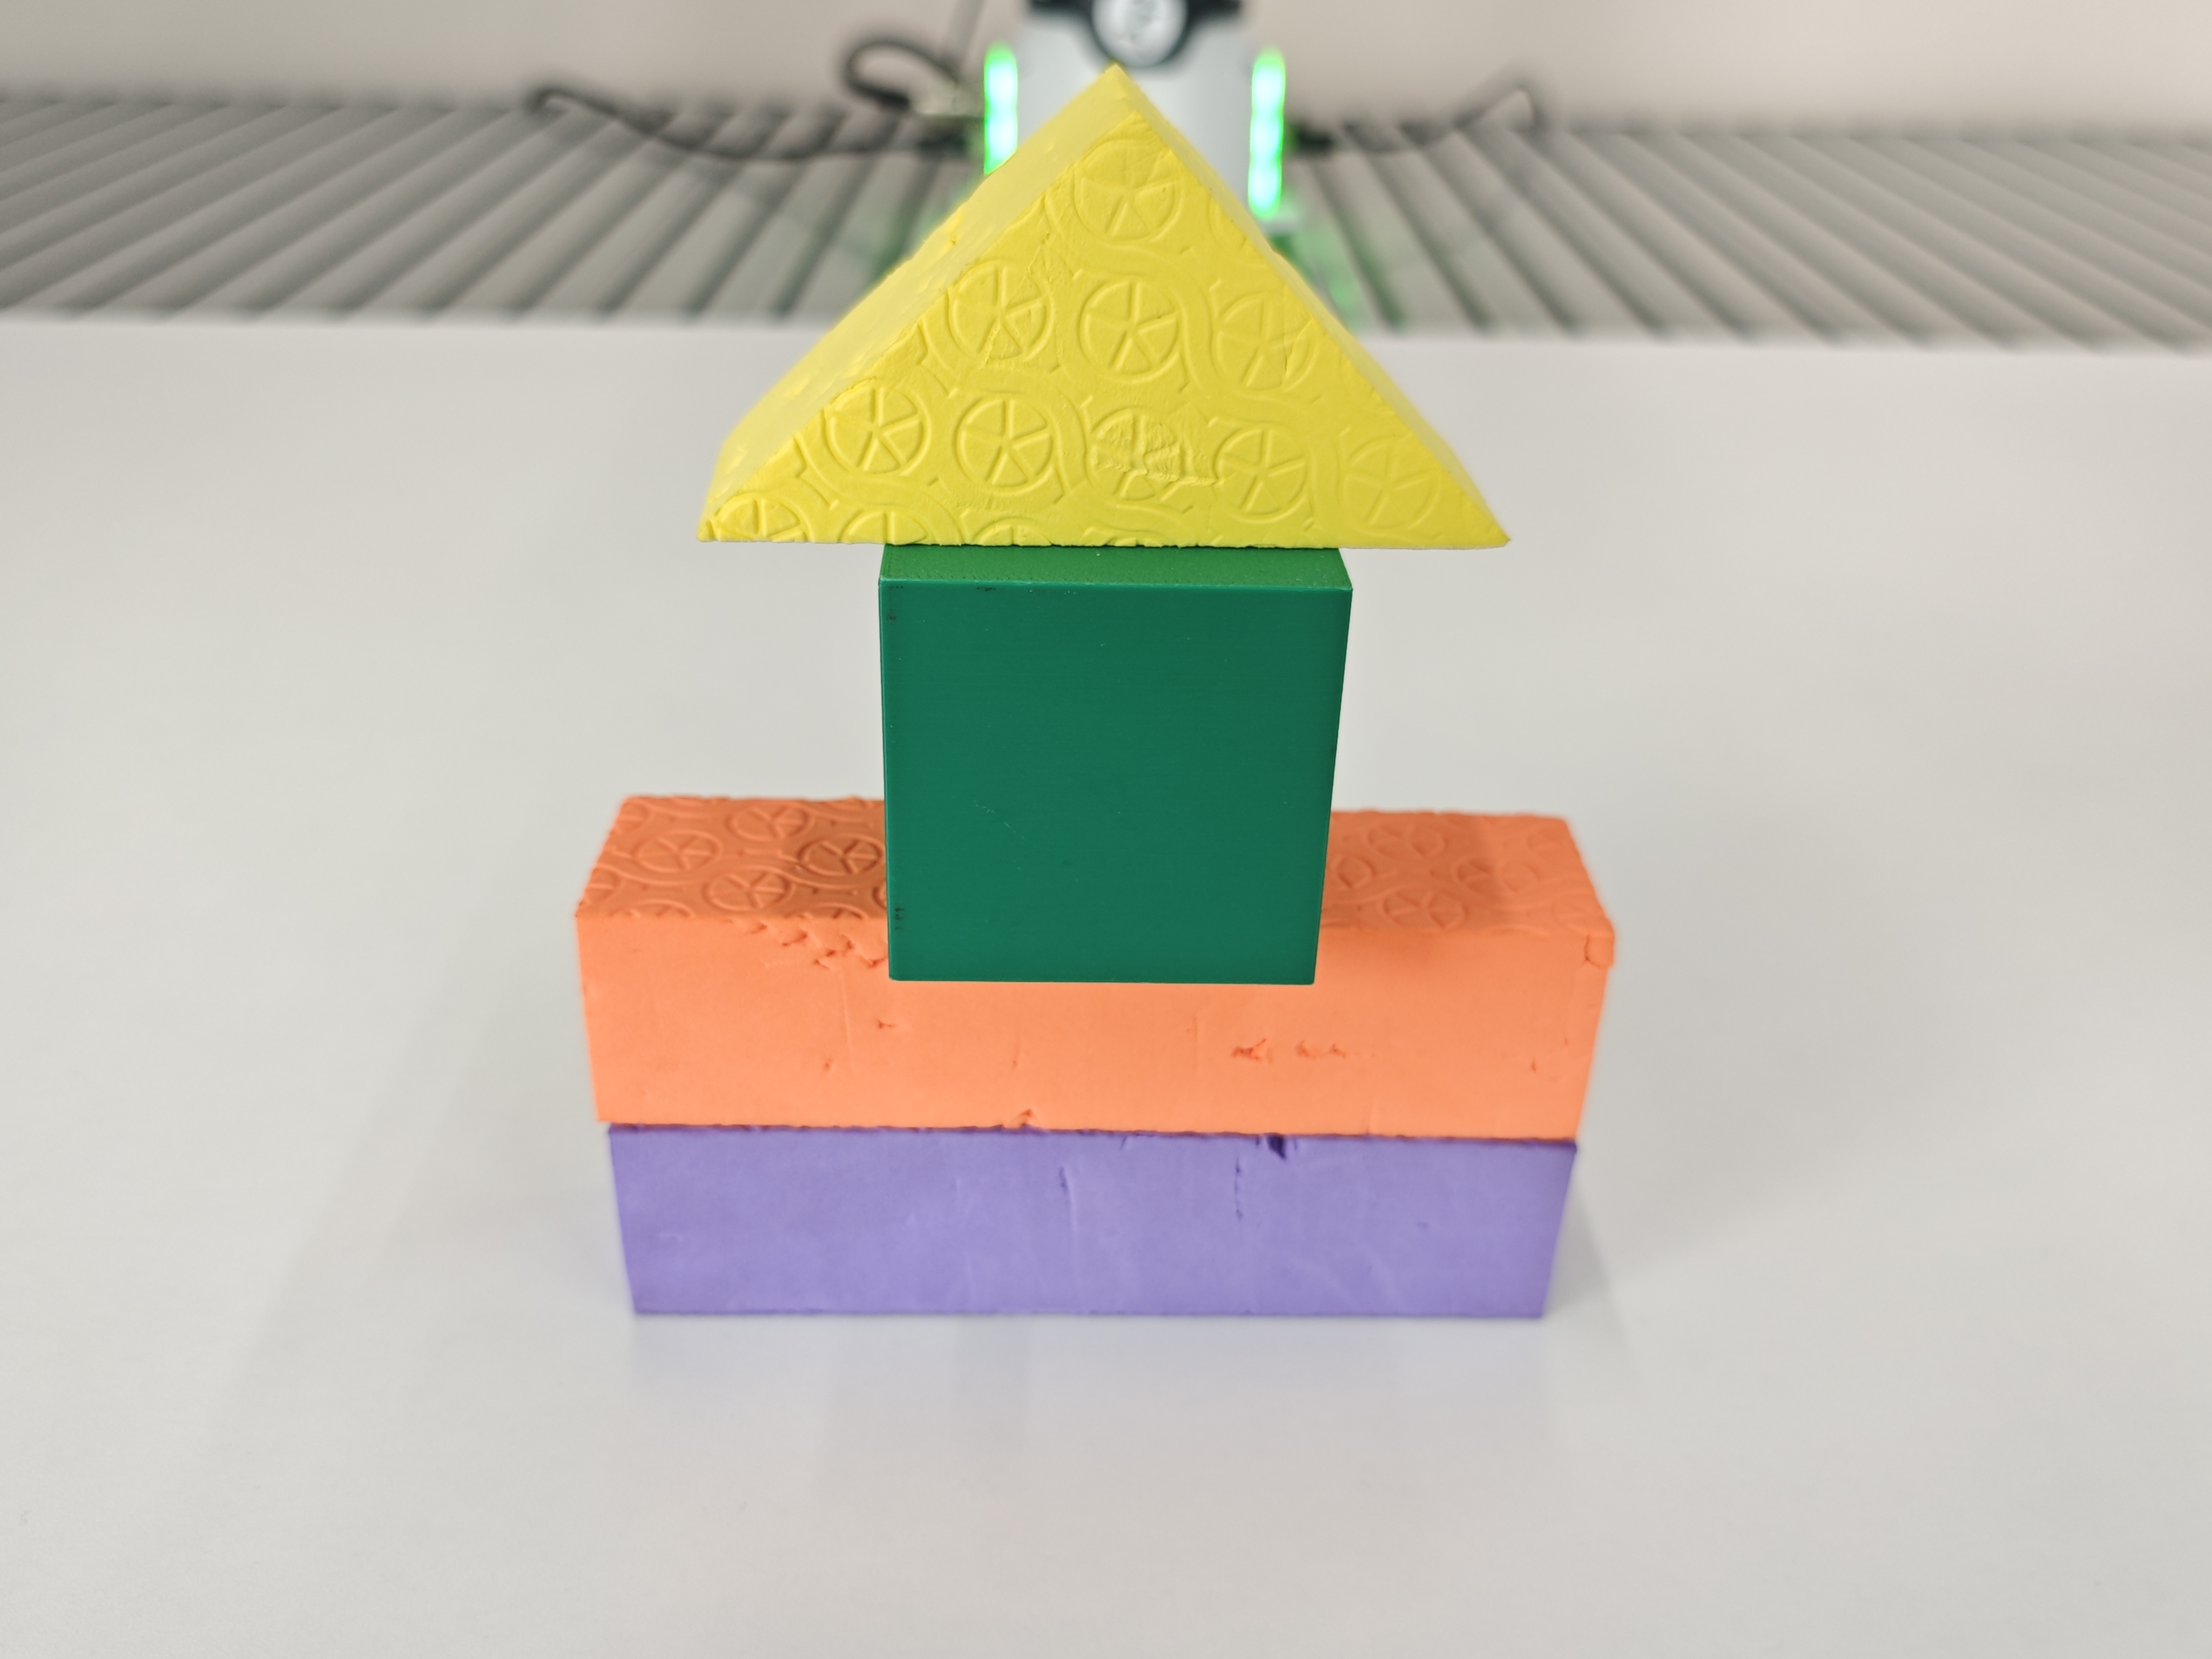
\includegraphics[height=1.0cm]{Figures/goal_images/medium2.jpg}
            \vspace{1pt}
        \end{minipage} 
        & Medium & 0/3 & 0/3 & 0/3 & 1/3 & \textbf{1/3} \\
        
        \begin{minipage}{0.3\textwidth}
            \centering \vspace{1pt}
            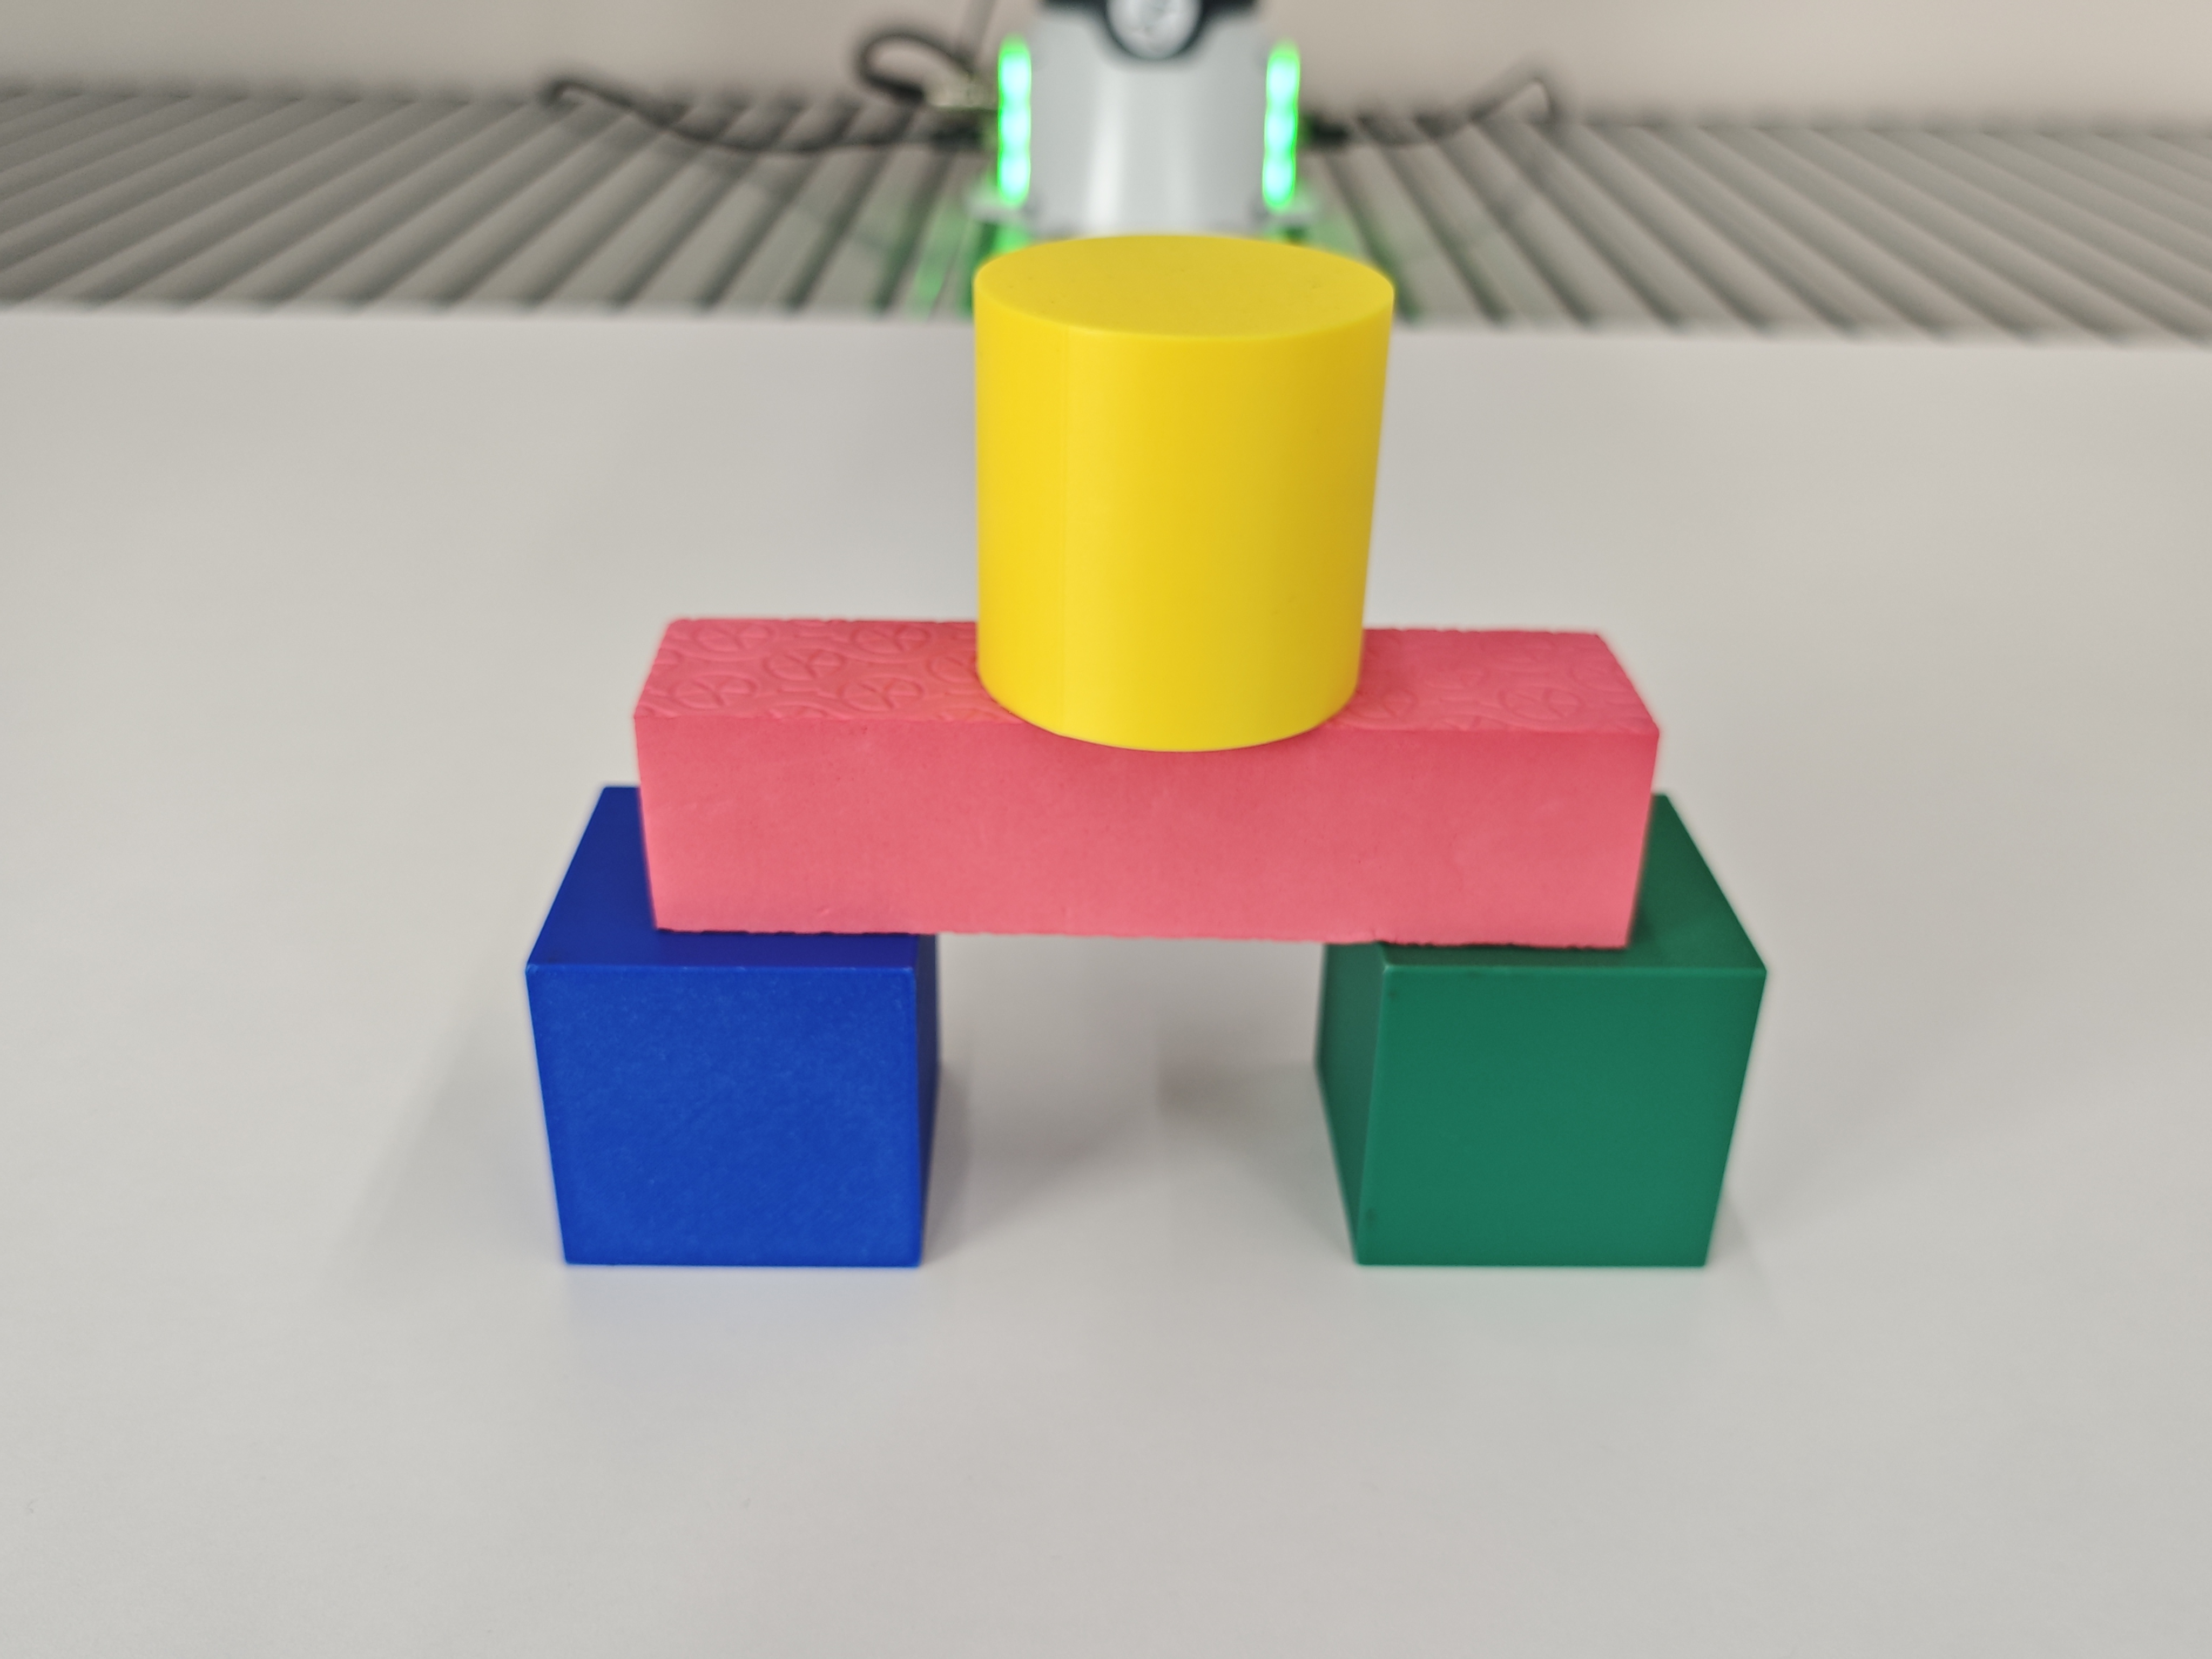
\includegraphics[height=1.0cm]{Figures/goal_images/medium3.jpg}
            \vspace{1pt}
        \end{minipage} 
        & Medium & 0/3 & 0/3 & 0/3 & 1/3 & \textbf{2/3} \\
        
        \begin{minipage}{0.3\textwidth}
            \centering \vspace{1pt}
            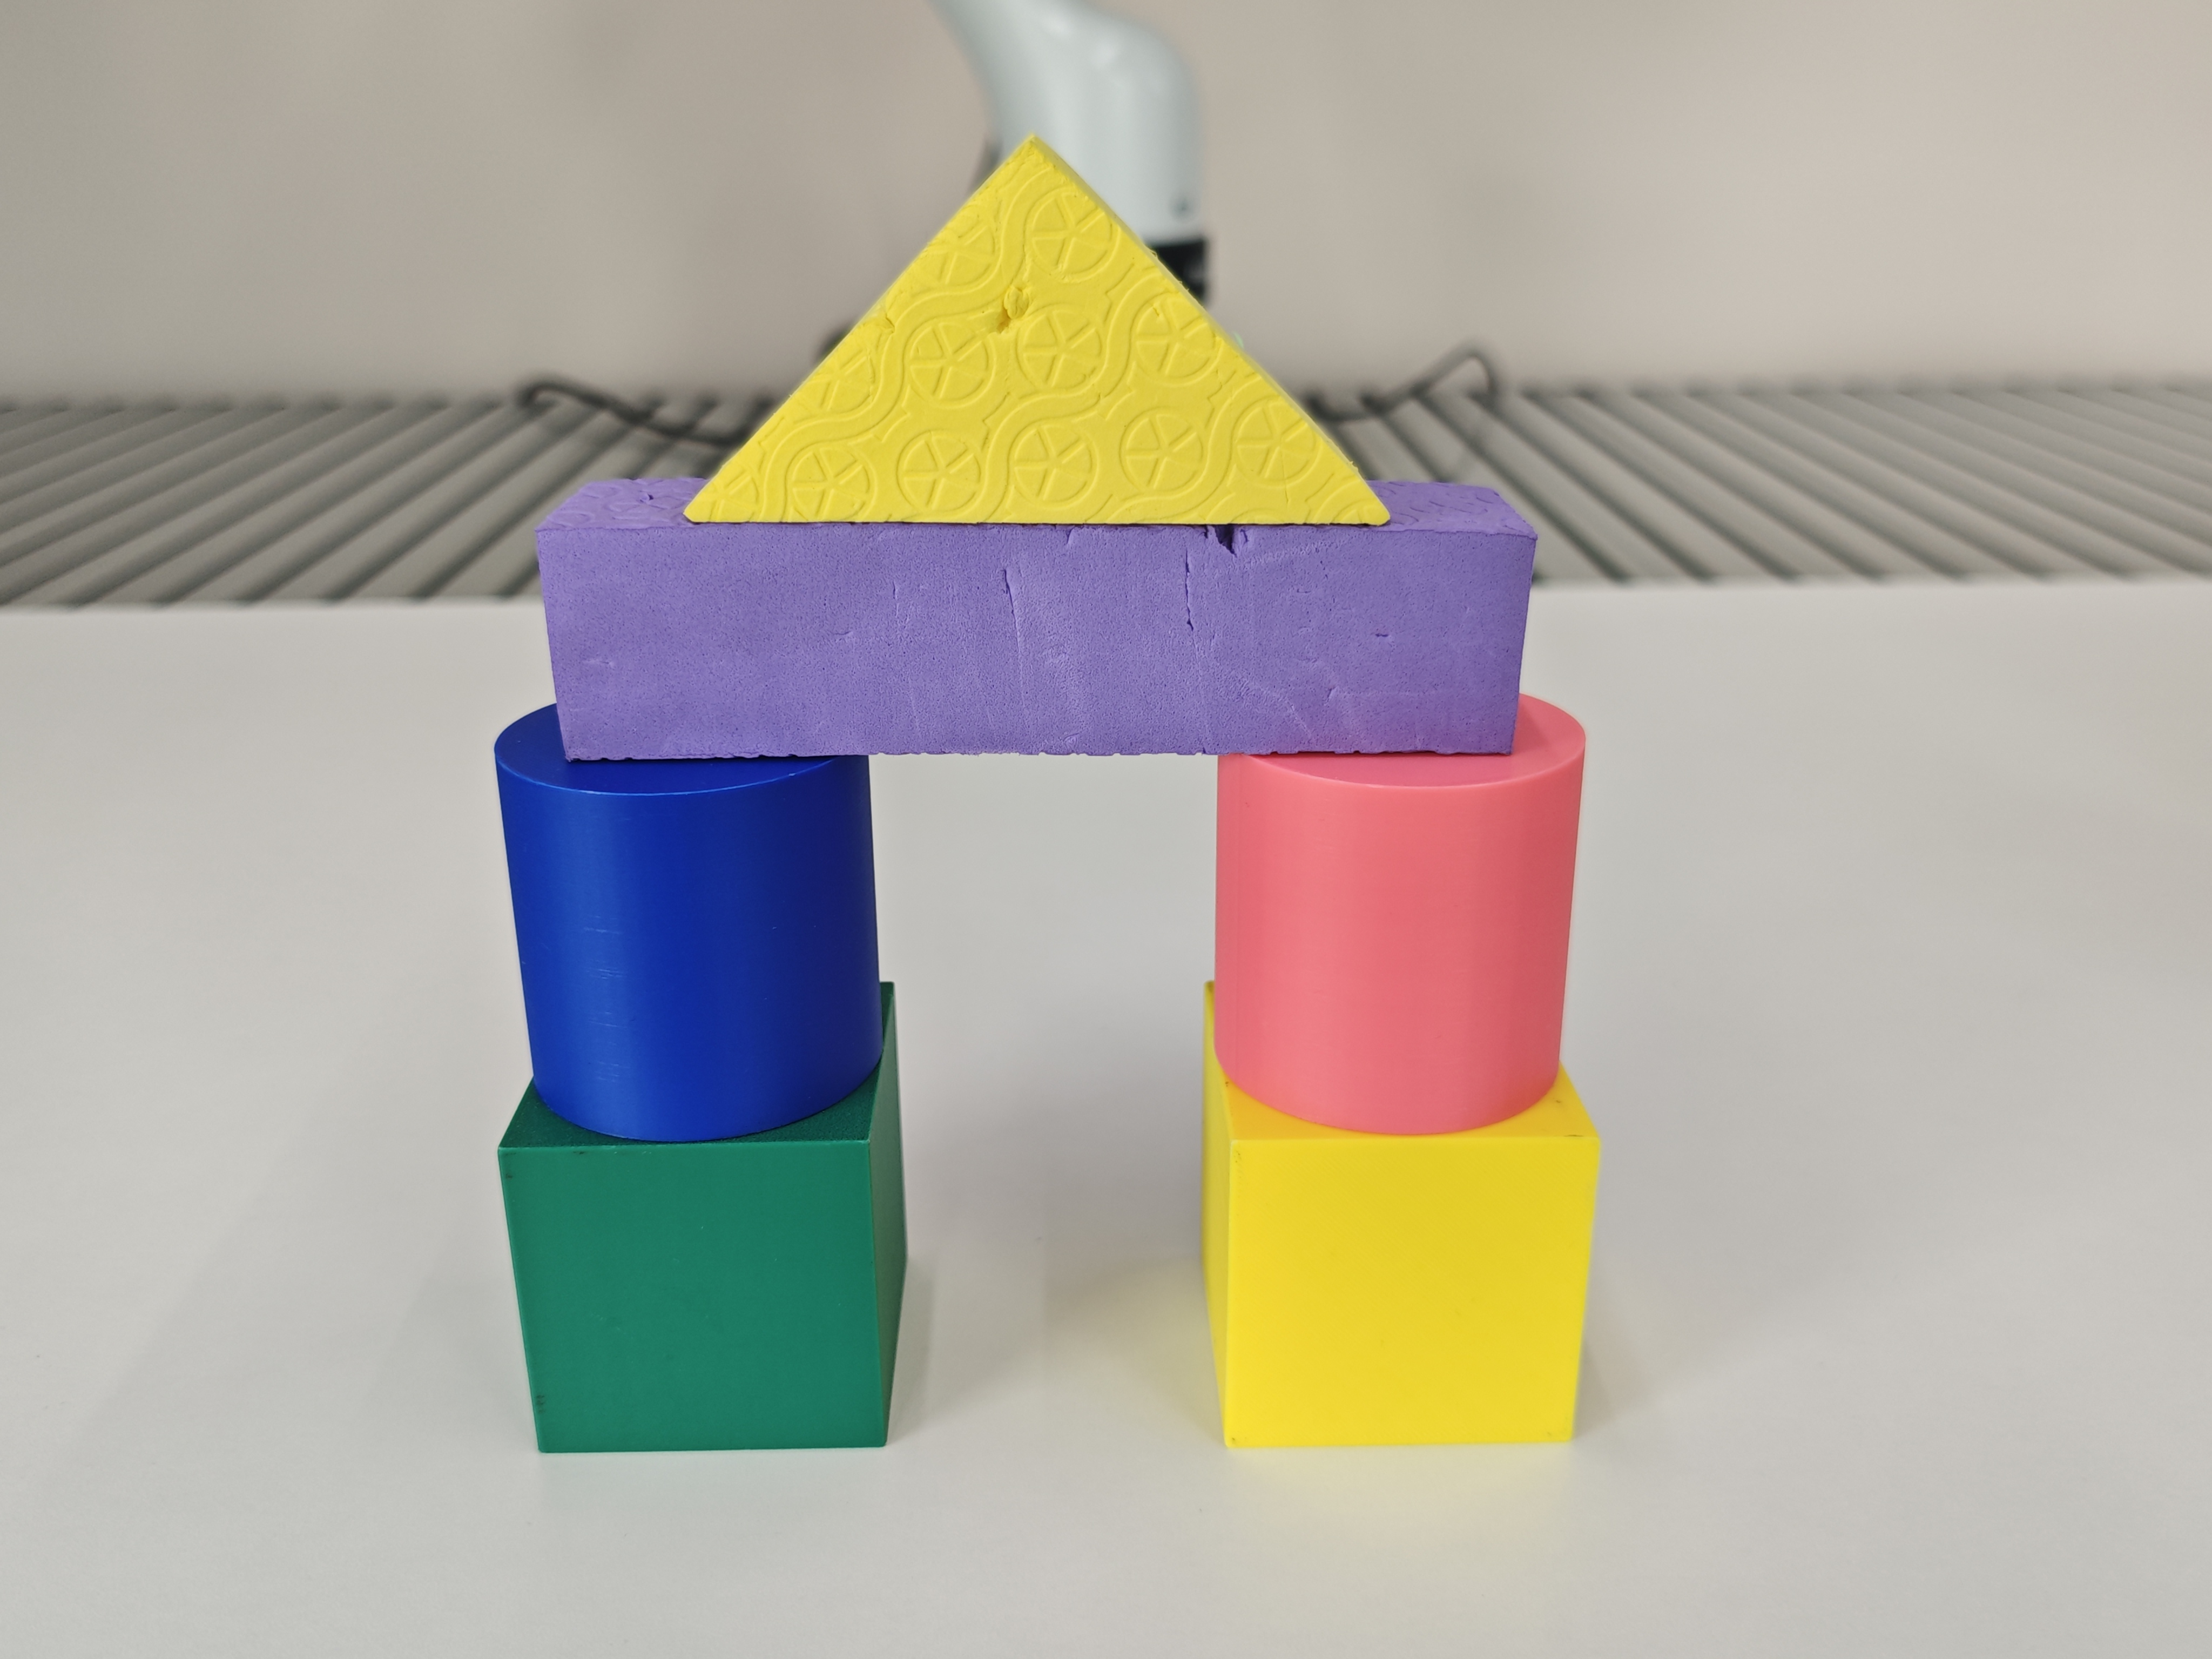
\includegraphics[height=1.0cm]{Figures/goal_images/hard1.jpg}
            \vspace{1pt}
        \end{minipage} 
        & Hard & 0/3 & 1/3 & 0/3 & 2/3 & \textbf{2/3} \\
        
        \begin{minipage}{0.3\textwidth}
            \centering \vspace{1pt}
            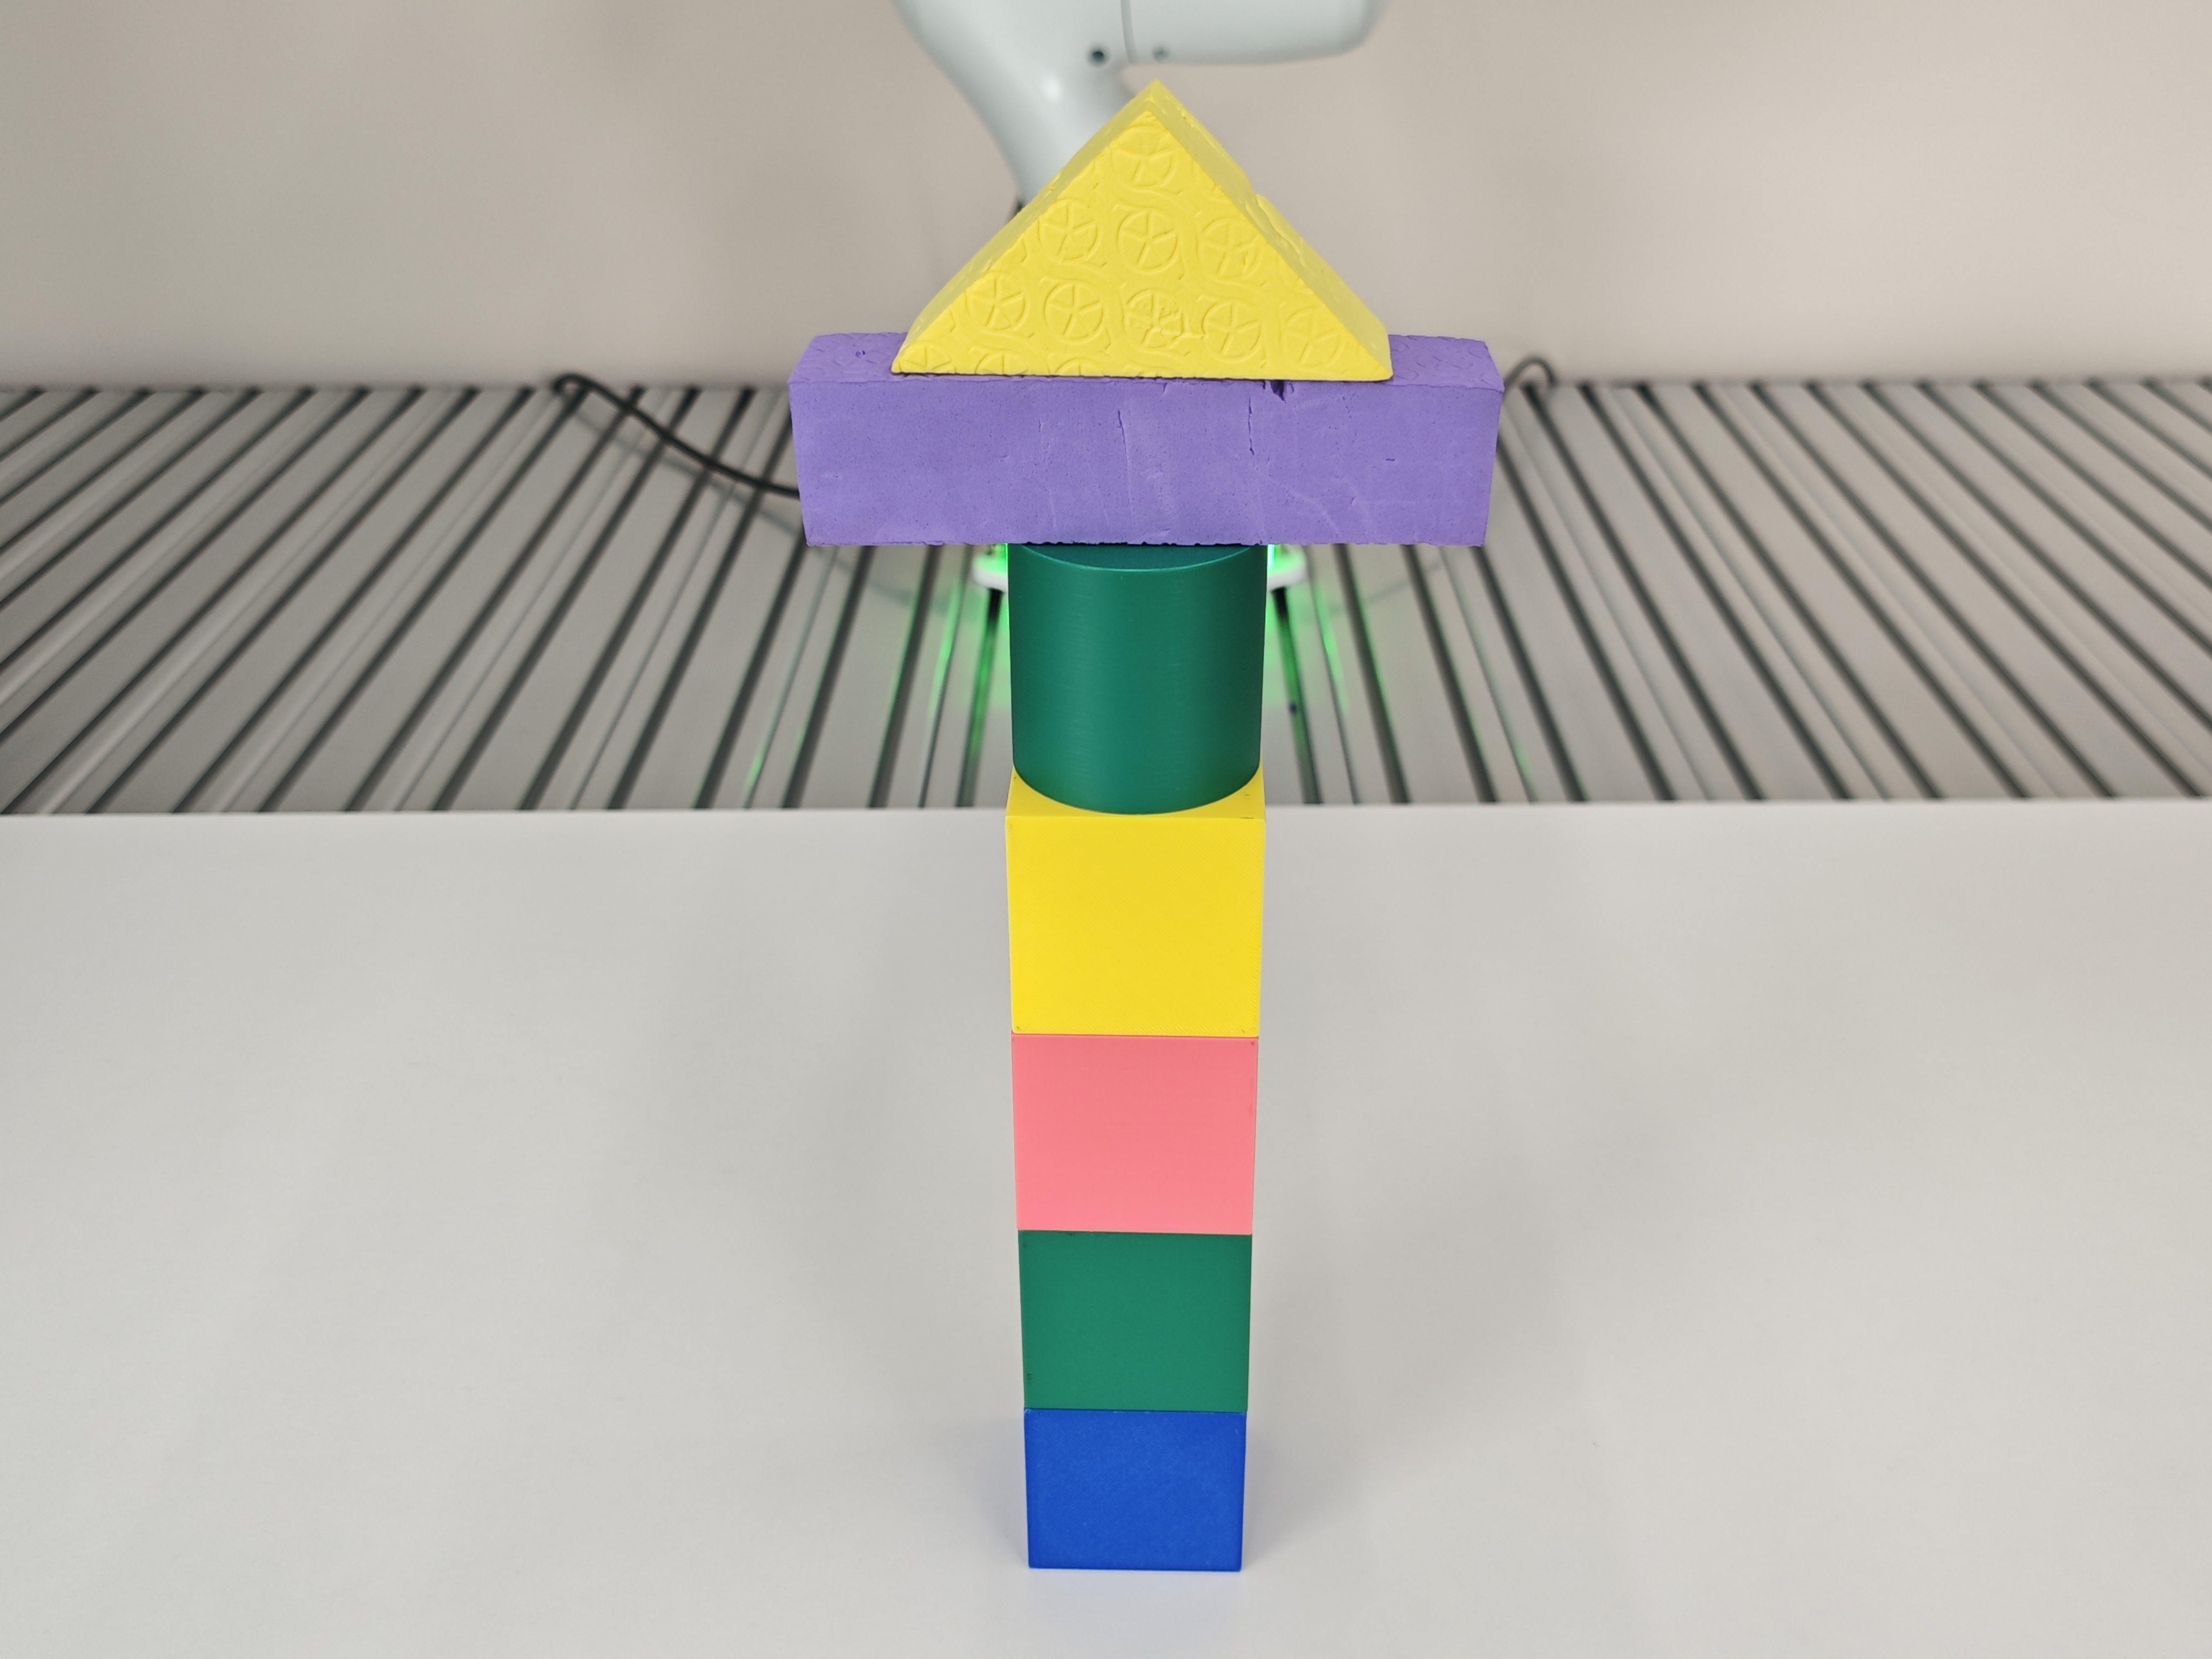
\includegraphics[height=1.0cm]{Figures/goal_images/hard2.jpg}
            \vspace{1pt}
        \end{minipage} 
        & Hard & 0/3 & 0/3 & 0/3 & 1/3 & \textbf{2/3} \\
        
        \begin{minipage}{0.3\textwidth}
            \centering \vspace{1pt}
            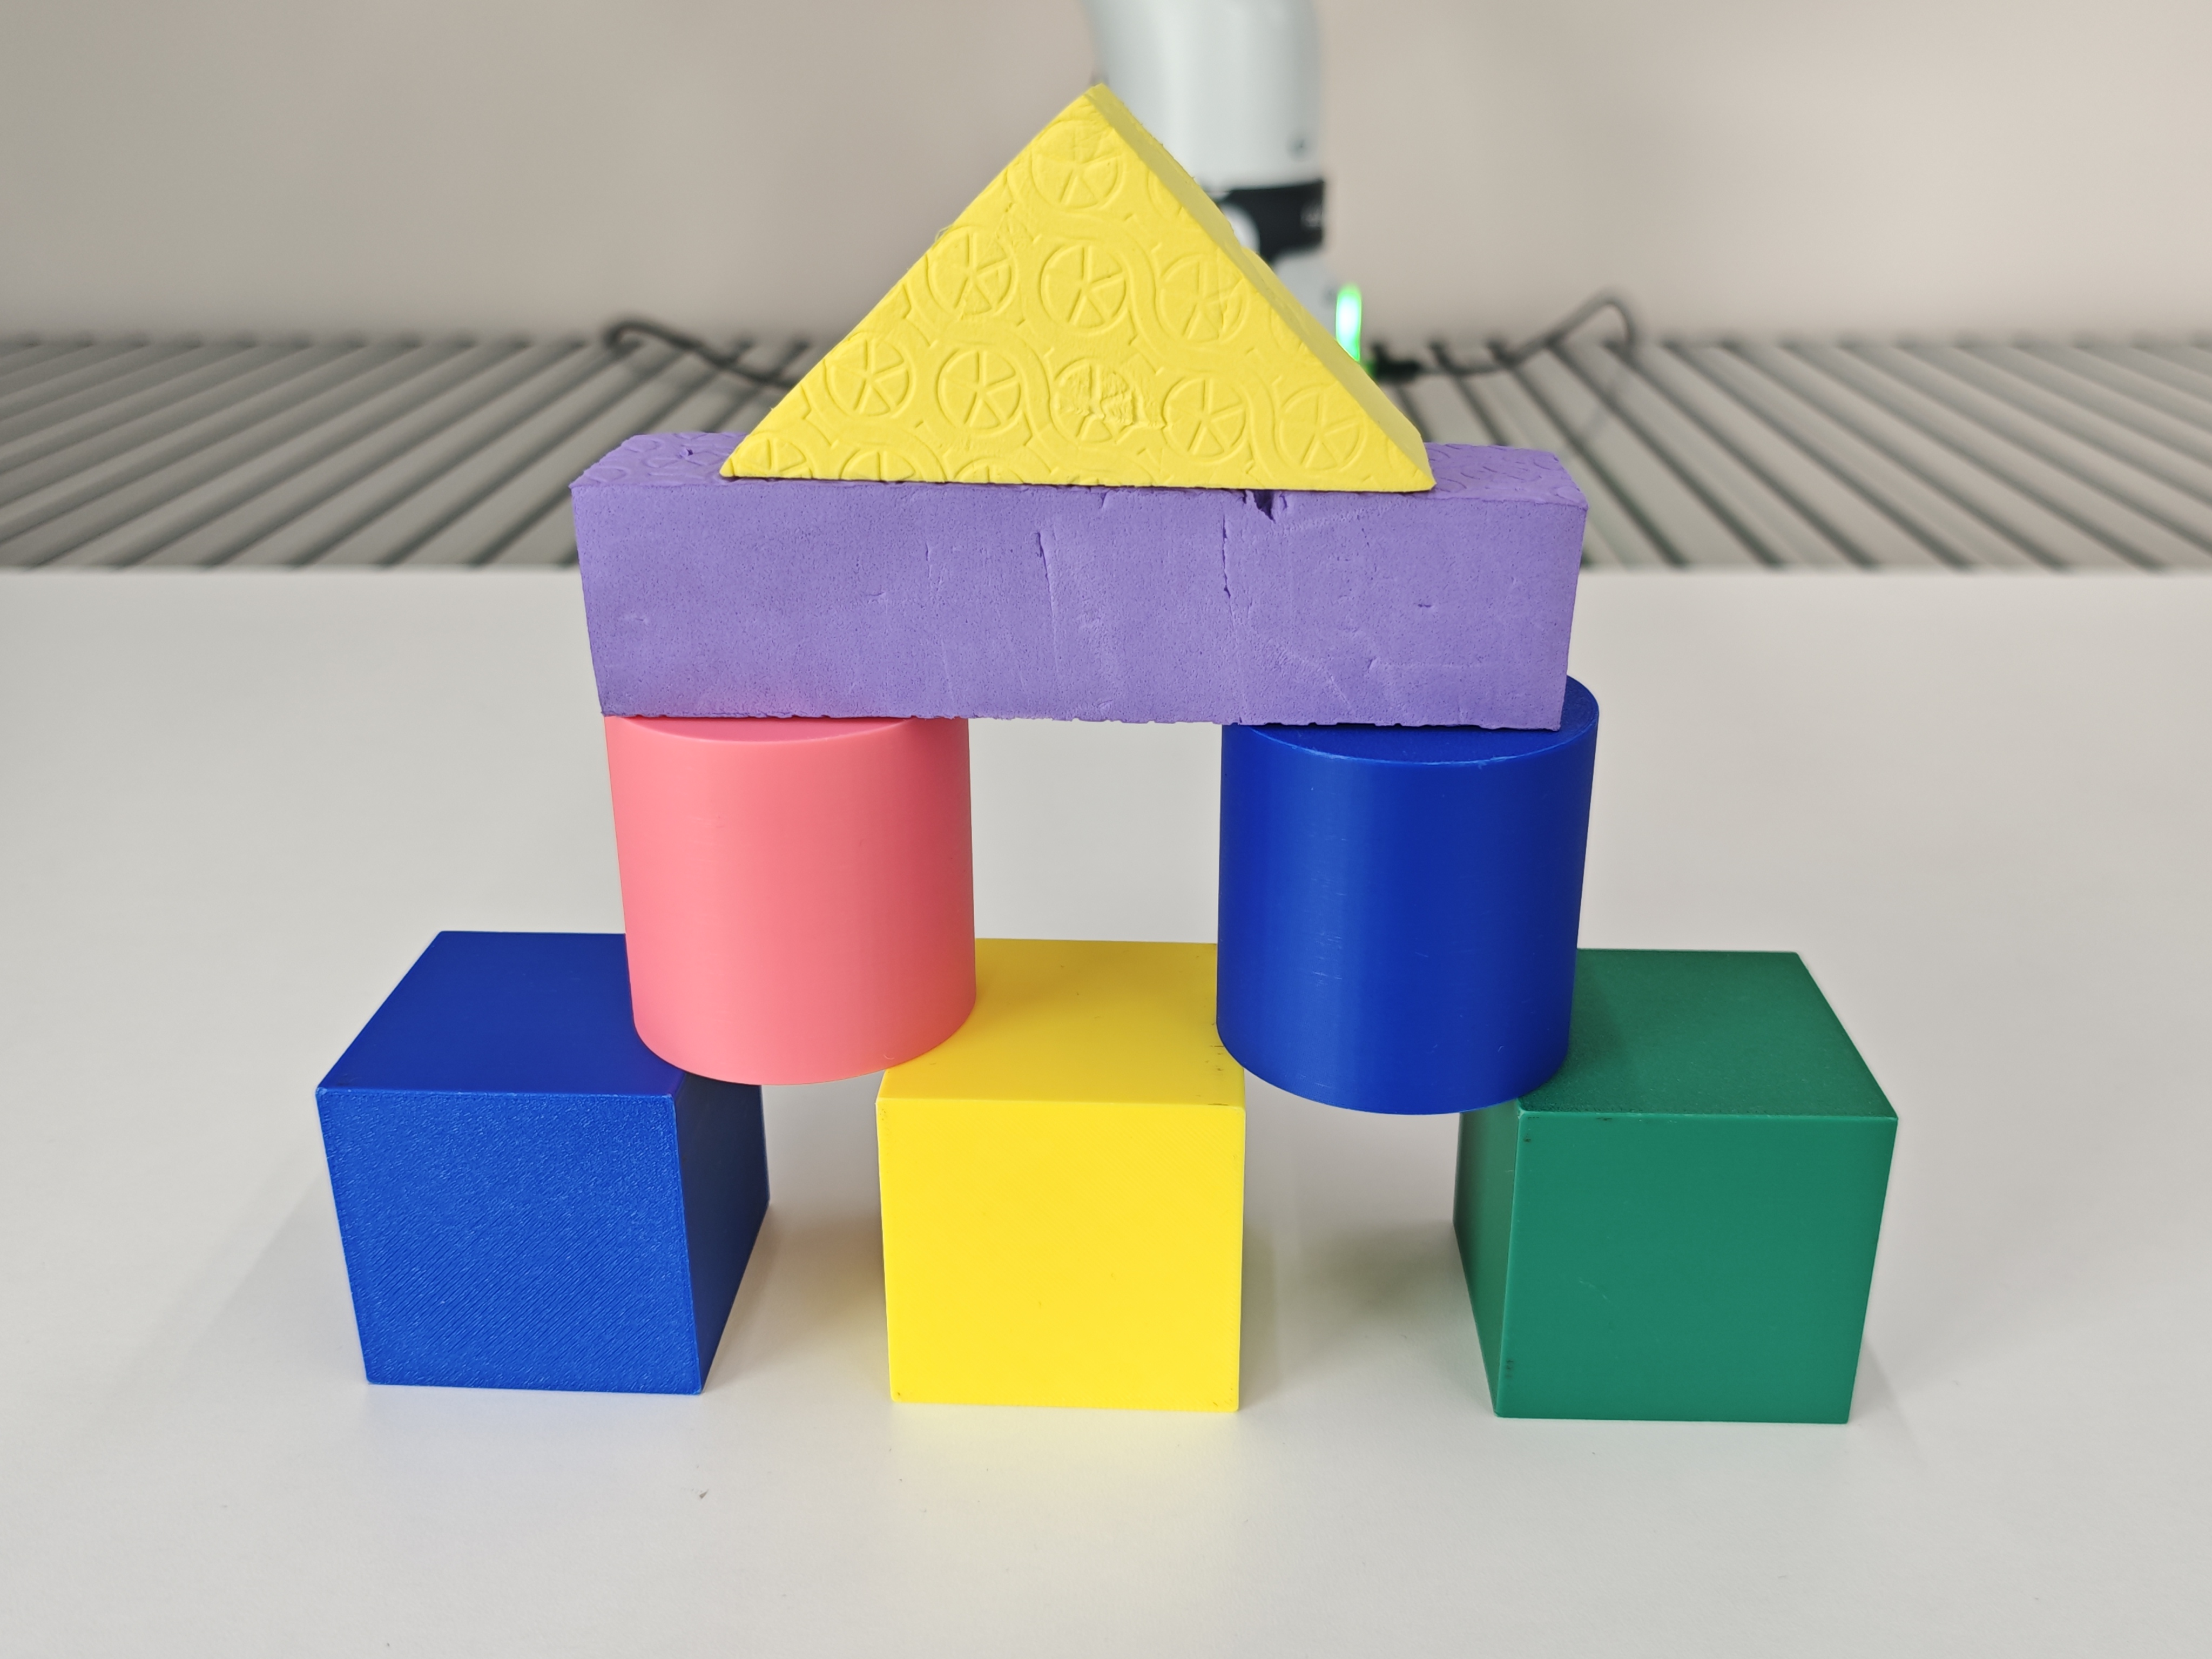
\includegraphics[height=1.0cm]{Figures/goal_images/hard3.jpg}
            \vspace{1pt}
        \end{minipage} 
        & Hard & 0/3 & 0/3 & 0/3 & 0/3 & \textbf{0/3} \\
        
        \multicolumn{2}{l}{\textbf{Building Avg (\%)}} & 18.5 & 25.9 & 25.9 & 48.2 & \textbf{63} \\
        \midrule
        
        % ==================== Section 2: 拆积木 ====================
        \multicolumn{7}{c}{\textit{Block Disassembly (Top-to-Bottom)} {\scriptsize $\vert$ \textit{Task $=$ Goal Image}}} \\
        \midrule
        \begin{minipage}{0.3\textwidth}
            \centering \vspace{1pt}
            \adjincludegraphics[height=0.8cm, trim={0 {.25\height} 0 {.25\height}}, clip]{Figures/goal_images/easy11.jpg}
            \vspace{1pt}
        \end{minipage} 
        & Easy & 2/3 & 3/3 & 2/3 & 2/3 & \textbf{3/3} \\
        
        \begin{minipage}{0.3\textwidth}
            \centering \vspace{1pt}
            \adjincludegraphics[height=0.8cm, trim={0 {.25\height} 0 {.25\height}}, clip]{Figures/goal_images/easy21.jpg}
            \vspace{1pt}
        \end{minipage} 
        & Easy & 2/3 & 2/3 & 3/3 & 3/3 & \textbf{3/3} \\
        
        \begin{minipage}{0.3\textwidth}
            \centering \vspace{1pt}
            \adjincludegraphics[height=0.8cm, trim={0 {.25\height} 0 {.25\height}}, clip]{Figures/goal_images/easy31.jpg}
            \vspace{1pt}
        \end{minipage} 
        & Easy & 1/3 & 1/3 & 1/3 & 2/3 & \textbf{2/3} \\
        
        \begin{minipage}{0.3\textwidth}
            \centering \vspace{1pt}
            \adjincludegraphics[height=0.8cm, trim={0 {.25\height} 0 {.25\height}}, clip]{Figures/goal_images/medium11.jpg}
            \vspace{1pt}
        \end{minipage} 
        & Medium & 1/3 & 0/3 & 0/3 & 1/3 & \textbf{2/3} \\
        
        \begin{minipage}{0.3\textwidth}
            \centering \vspace{1pt}
            \adjincludegraphics[height=0.8cm, trim={0 {.25\height} 0 {.25\height}}, clip]{Figures/goal_images/medium21.jpg}
            \vspace{1pt}
        \end{minipage} 
        & Medium & 0/3 & 0/3 & 1/3 & 2/3 & \textbf{2/3} \\
        
        \begin{minipage}{0.3\textwidth}
            \centering \vspace{1pt}
            \adjincludegraphics[height=0.8cm, trim={0 {.25\height} 0 {.25\height}}, clip]{Figures/goal_images/medium31.jpg}
            \vspace{1pt}
        \end{minipage} 
        & Medium & 1/3 & 0/3 & 1/3 & 2/3 & \textbf{3/3} \\
        
        \begin{minipage}{0.3\textwidth}
            \centering \vspace{1pt}
            \adjincludegraphics[height=0.8cm, trim={0 {.25\height} 0 {.25\height}}, clip]{Figures/goal_images/hard11.jpg}
            \vspace{1pt}
        \end{minipage} 
        & Hard & 1/3 & 1/3 & 2/3 & 2/3 & \textbf{2/3} \\
        
        \begin{minipage}{0.3\textwidth}
            \centering \vspace{1pt}
            \adjincludegraphics[height=0.8cm, trim={0 {.25\height} 0 {.25\height}}, clip]{Figures/goal_images/hard21.jpg}
            \vspace{1pt}
        \end{minipage} 
        & Hard & 0/3 & 0/3 & 0/3 & 2/3 & \textbf{2/3} \\
        
        \begin{minipage}{0.3\textwidth}
            \centering \vspace{1pt}
            \adjincludegraphics[height=0.8cm, trim={0 {.25\height} 0 {.25\height}}, clip]{Figures/goal_images/hard31.jpg}
            \vspace{1pt}
        \end{minipage} 
        & Hard & 0/3 & 0/3 & 1/3 & 1/3 & \textbf{2/3} \\
        
        \multicolumn{2}{l}{\textbf{Disassembly Avg (\%)}} & 29.6 & 25.9 & 40.7 & 63 & \textbf{77.8} \\
        \midrule

        % ==================== Section 3: Hide 案例 ====================
        \multicolumn{7}{c}{\textit{Long-Horizon Memorize and Restore} {\scriptsize $\vert$ \textit{Task $=$ Initial State + Instruction}}} \\
        \midrule
        % Blue cube (top of tower) -- no disassembly needed
        \begin{minipage}{0.3\textwidth}
            \centering \vspace{1pt}
            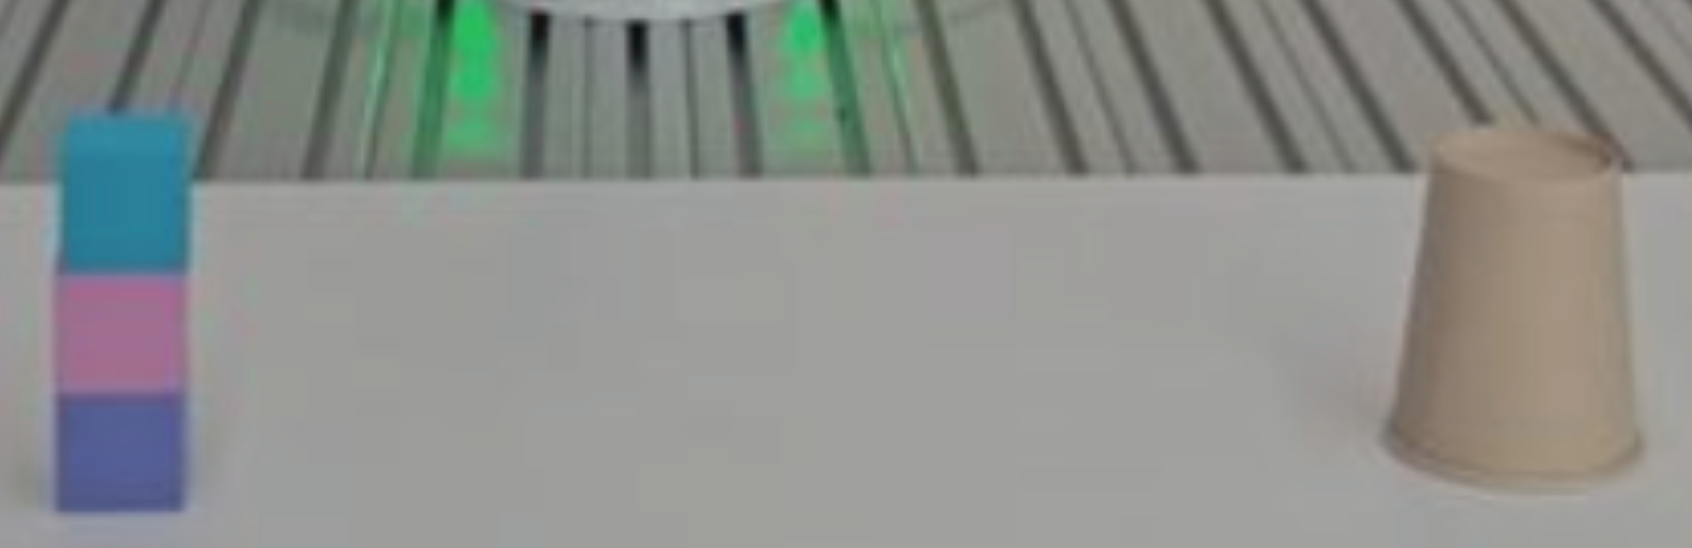
\includegraphics[height=1.2cm]{Figures/goal_images/hide.png}
            \\[-3pt]
            {\scriptsize \textit{Hide the \textbf{blue} cube with the brown cup, then restore.}}
            \vspace{1pt}
        \end{minipage}
        & Medium & ?/3 & ?/3 & ?/3 & ?/3 & \textbf{?/3} \\
        
        % Purple cube (bottom of tower) -- must disassemble tower first
        \begin{minipage}{0.3\textwidth}
            \centering \vspace{1pt}
            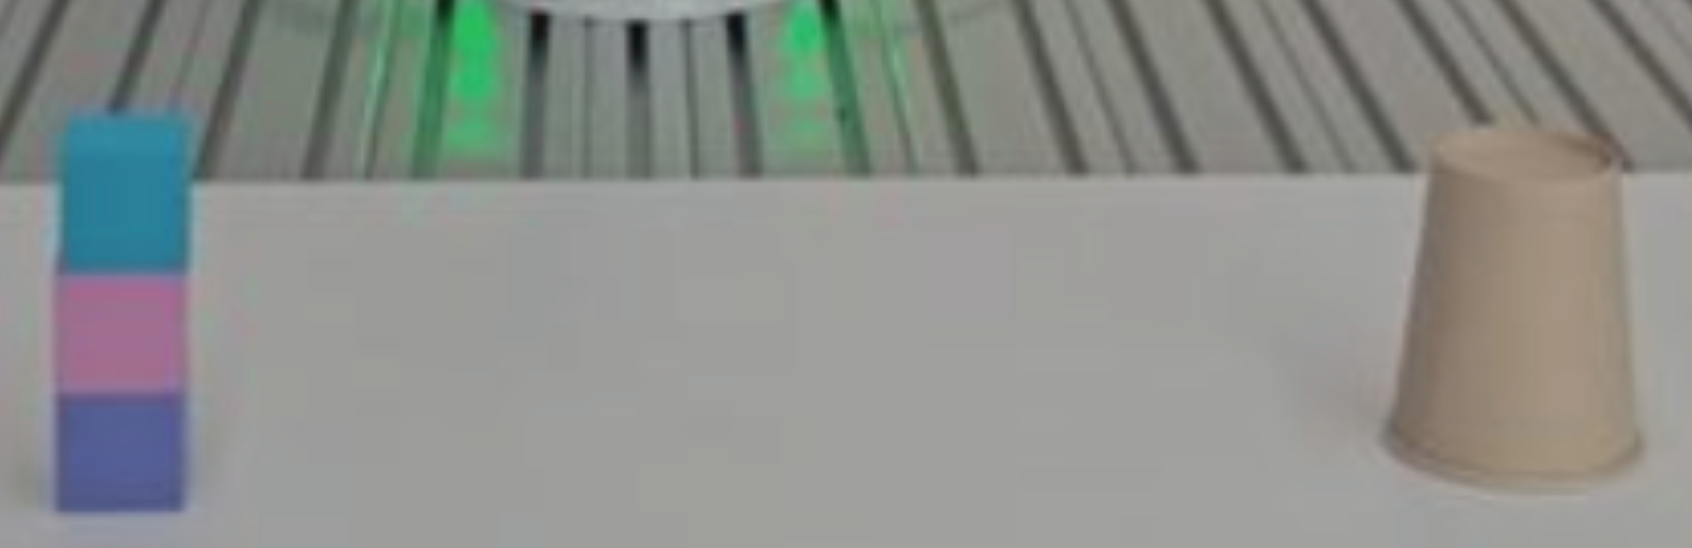
\includegraphics[height=1.2cm]{Figures/goal_images/hide.png}
            \\[-3pt]
            {\scriptsize \textit{Hide the \textbf{purple} cube with the brown cup, then restore.}}
            \vspace{1pt}
        \end{minipage}
        & Hard & 0/3 & 0/3 & 2/3 & 3/5 & \textbf{4/4} \\
        
        \cmidrule(lr){1-7}
        \multicolumn{2}{l}{\textbf{Overall Real-World Avg (\%)}} & 26.3 & 35.5 & 39.5 & 67.0 & \textbf{74.3} \\
        \bottomrule
    \end{tabular}
}
\end{table}
\subsubsection{Detailed Results of Simulation Manipulation}

To provide a comprehensive understanding of how our proposed components contribute to the overall performance across different model capacities, we present the detailed ablation results on the RLBench multi-step tasks in Table~\ref{tab:sim_detailed_ablation}. This section expands upon the macro-level analysis by reporting the execution success rates for all three model scales (8B, 32B, and 235B) under three architectural configurations: the Full Model, the variant without Spatio-Temporal Fusion Tokens (w/o STF-Tokens), and the variant without the episodic memory log (w/o Memory).

As observed in the detailed breakdown, removing the episodic memory results in a near-complete collapse across tasks that strictly require cross-step state tracking and occlusion reasoning (e.g., \textit{Bridge Between Towers} and \textit{Stack Colors}). The memory-ablated model only retains partial capability on tasks where intermediate spatial constraints can be somewhat inferred directly from the current visual frame (e.g., \textit{Place in Cont.}). Furthermore, the results highlight a clear capability scaling law in handling extreme occlusion: while the 235B Full Model achieves near-perfect execution on the \textit{Cover Top/Bottom} tasks (92.0\% and 96.0\% success rates), the 8B model struggles significantly (40.0\% and 16.0\%), and the 32B model shows intermediate performance (84.0\% and 68.0\%). This indicates that robust occlusion recovery heavily relies on the emergent semantic reasoning capacity of larger parameter scales.

Conversely, removing STF-Tokens while retaining the Causal Spatio-Temporal Graph (CSTG) generally preserves the logical progression of the tasks but introduces significant variance in spatial execution precision. This degradation in physical accuracy is evident across all model scales, particularly on contact-rich tasks like \textit{Stack Five Colors} (e.g., dropping from 72.0\% to 48.0\% for the 32B model, and 60.0\% to 40.0\% for 8B). This explicitly confirms our hypothesis: while memory ensures the correct semantic sequence is planned, explicit 3D geometric grounding (STF-Tokens) is strictly required to stabilize the physical execution of those plans, even for highly capable VLMs.

\begin{table}[htbp]
    \centering
    \caption{\textbf{Comprehensive Ablation Results in Simulation.} Success rates (\%) across 8 multi-step RLBench tasks. We compare the full RoboStream pipeline against variants removing Spatio-Temporal Fusion Tokens (w/o STF-Tokens), the episodic memory log (w/o Memory), \textbf{or both (w/o Both)} across 8B, 32B, and 235B scales. Data is averaged over 25 independent episodes per task. The 235B results correspond to the macro ablation study presented in the main text.}
    \label{tab:sim_detailed_ablation}
    \renewcommand{\arraystretch}{1.05} 
    \setlength{\tabcolsep}{3pt} 
    
    \resizebox{\textwidth}{!}{
    \begin{tabular}{c l c c c c c c c c c}
        \toprule
        \textbf{Scale} & \textbf{Variant} & \begin{tabular}{@{}c@{}}\textbf{Bridge} \\ \textbf{Between}\end{tabular} & \begin{tabular}{@{}c@{}}\textbf{Cover} \\ \textbf{Bottom}\end{tabular} & \begin{tabular}{@{}c@{}}\textbf{Cover} \\ \textbf{Top}\end{tabular} & \begin{tabular}{@{}c@{}}\textbf{Place in} \\ \textbf{Cont.}\end{tabular} & \begin{tabular}{@{}c@{}}\textbf{Place in} \\ \textbf{Cont. (H)}\end{tabular} & \begin{tabular}{@{}c@{}}\textbf{Stack} \\ \textbf{Five}\end{tabular} & \begin{tabular}{@{}c@{}}\textbf{Stack} \\ \textbf{Three}\end{tabular} & \begin{tabular}{@{}c@{}}\textbf{Unstack} \\ \textbf{\& Stack}\end{tabular} & \textbf{Avg} \\
        \midrule
        
        \multirow{4}{*}{\textbf{8B}} 
        & Full Model & \textbf{76.0} & \textbf{16.0} & \textbf{40.0} & \textbf{100.0} & \textbf{24.0} & \textbf{60.0} & \textbf{96.0} & \textbf{52.0} & \textbf{58.0} \\
        & w/o STF-Tokens & \underline{68.0} & \underline{8.0} & \underline{24.0} & \textbf{100.0} & \underline{12.0} & \underline{40.0} & \underline{88.0} & \underline{24.0} & \underline{45.5} \\
        & w/o Memory & 0.0 & 0.0 & 0.0 & \textbf{100.0} & 0.0 & 0.0 & 0.0 & 0.0 & 12.5 \\
        & w/o Both & 0.0 & 0.0 & 0.0 & 88.0 & 0.0 & 0.0 & 0.0 & 0.0 & 11.0 \\
        \cmidrule{1-11}
        
        \multirow{4}{*}{\textbf{32B}} 
        & Full Model & \textbf{88.0} & \textbf{68.0} & \textbf{84.0} & \textbf{100.0} & \textbf{76.0} & \textbf{72.0} & \textbf{96.0} & \textbf{76.0} & \textbf{82.5} \\
        & w/o STF-Tokens & \underline{80.0} & \underline{52.0} & \underline{68.0} & \textbf{100.0} & \underline{60.0} & \underline{48.0} & \underline{88.0} & \underline{56.0} & \underline{69.0} \\
        & w/o Memory & 0.0 & 0.0 & 0.0 & \underline{56.0} & 12.0 & 0.0 & 0.0 & 0.0 & 8.5 \\
        & w/o Both & 0.0 & 0.0 & 0.0 & 48.0 & 0.0 & 0.0 & 0.0 & 0.0 & 6.0 \\
        \cmidrule{1-11}
        
        \multirow{4}{*}{\textbf{235B}} 
        & Full Model & \textbf{88.0} & \textbf{96.0} & \textbf{92.0} & \textbf{100.0} & \textbf{88.0} & \textbf{80.0} & \textbf{96.0} & \textbf{84.0} & \textbf{90.5} \\
        & w/o STF-Tokens & \underline{72.0} & \underline{88.0} & \underline{84.0} & \textbf{100.0} & \underline{72.0} & \underline{60.0} & \textbf{96.0} & \underline{64.0} & \underline{79.5} \\
        & w/o Memory & 0.0 & 0.0 & 0.0 & \underline{92.0} & 24.0 & 0.0 & 0.0 & 0.0 & 14.5 \\
        & w/o Both & 0.0 & 0.0 & 0.0 & 84.0 & 12.0 & 0.0 & 0.0 & 0.0 & 12.0 \\
        
        \bottomrule
    \end{tabular}
    }
\end{table}

\subsection{Additional Experiments}
\subsubsection{Runtime Scaling of RoboStream}
% 我们选取了一个7步的hard拆积木任务，在单张A100 GPU上对RoboStream-8B进行评估，设置滑动窗口长度为3，并且分模块进行耗时统计，①感知模块：涉及到基于Qwen3-VL-8B的open-vocabulary object parsing以及基于SAM3的segmentation②场景图构建模块：包括事件检测和场景图计算 ③VLM推理模块，涉及到基于Qwen3-VL-8B的推理。
% 如表1所示，感知模块与场景图构建模块的耗时随着时间步长增加保持稳定，VLM推理模块的耗时先增加后保持稳定，且增长幅度较小，验证了STF-tokens和CSTG的可拓展性。
We evaluate RoboStream-8B on a challenging 7-step block-unstacking task using a single NVIDIA A100 GPU with a sliding window length of 3. To analyze computational efficiency, we perform a modular latency breakdown across the perception module (comprising Qwen3-VL-8B-based open-vocabulary object parsing and SAM3-based segmentation), the scene graph construction module (encompassing event detection and scene graph computation), and the VLM inference module. As reported in Table 1, the execution time for the perception and scene graph modules remains stable across time steps, while the VLM inference latency exhibits a marginal initial increase before stabilizing. This minimal growth in overhead empirically validates the scalability of our proposed STF-tokens and CSTG frameworks.
\begin{table}[h]
\centering
\caption{\textbf{Inference Latency Analysis across Modules.} Average processing time (s) for seven sequential steps. }
\label{tab:latency_breakdown}
% 使用 tabular* 配合 @{\extracolsep{\fill}} 自动撑满宽度
\begin{tabular*}{\textwidth}{@{\extracolsep{\fill}} l cccc @{}}
\toprule
\textbf{Steps} & 
\textbf{Perception} & 
\textbf{CSTG Construct} & 
\textbf{VLM Inference} & 
\textbf{Total Latency} \\
\midrule
Step 1 & 0.24 & 0.14 & 6.56 & 6.94 \\
Step 2 & 0.22 & 0.15 & 6.92 & 7.29 \\
Step 3 & 0.30 & 0.17 & 7.44 & 7.91 \\
Step 4 & 0.25 & 0.17 & 7.31 & 7.73 \\
Step 5 & 0.25 & 0.17 & 7.44 & 7.86 \\
Step 6 & 0.22 & 0.16 & 7.42 & 7.80 \\
Step 7 & 0.24 & 0.17 & 7.38 & 7.79 \\
\midrule
\textbf{Avg} & 0.25 & 0.16 & 7.21 & 7.62 \\
\bottomrule
\end{tabular*}
\end{table}

\begin{figure}[p]
    \centering
    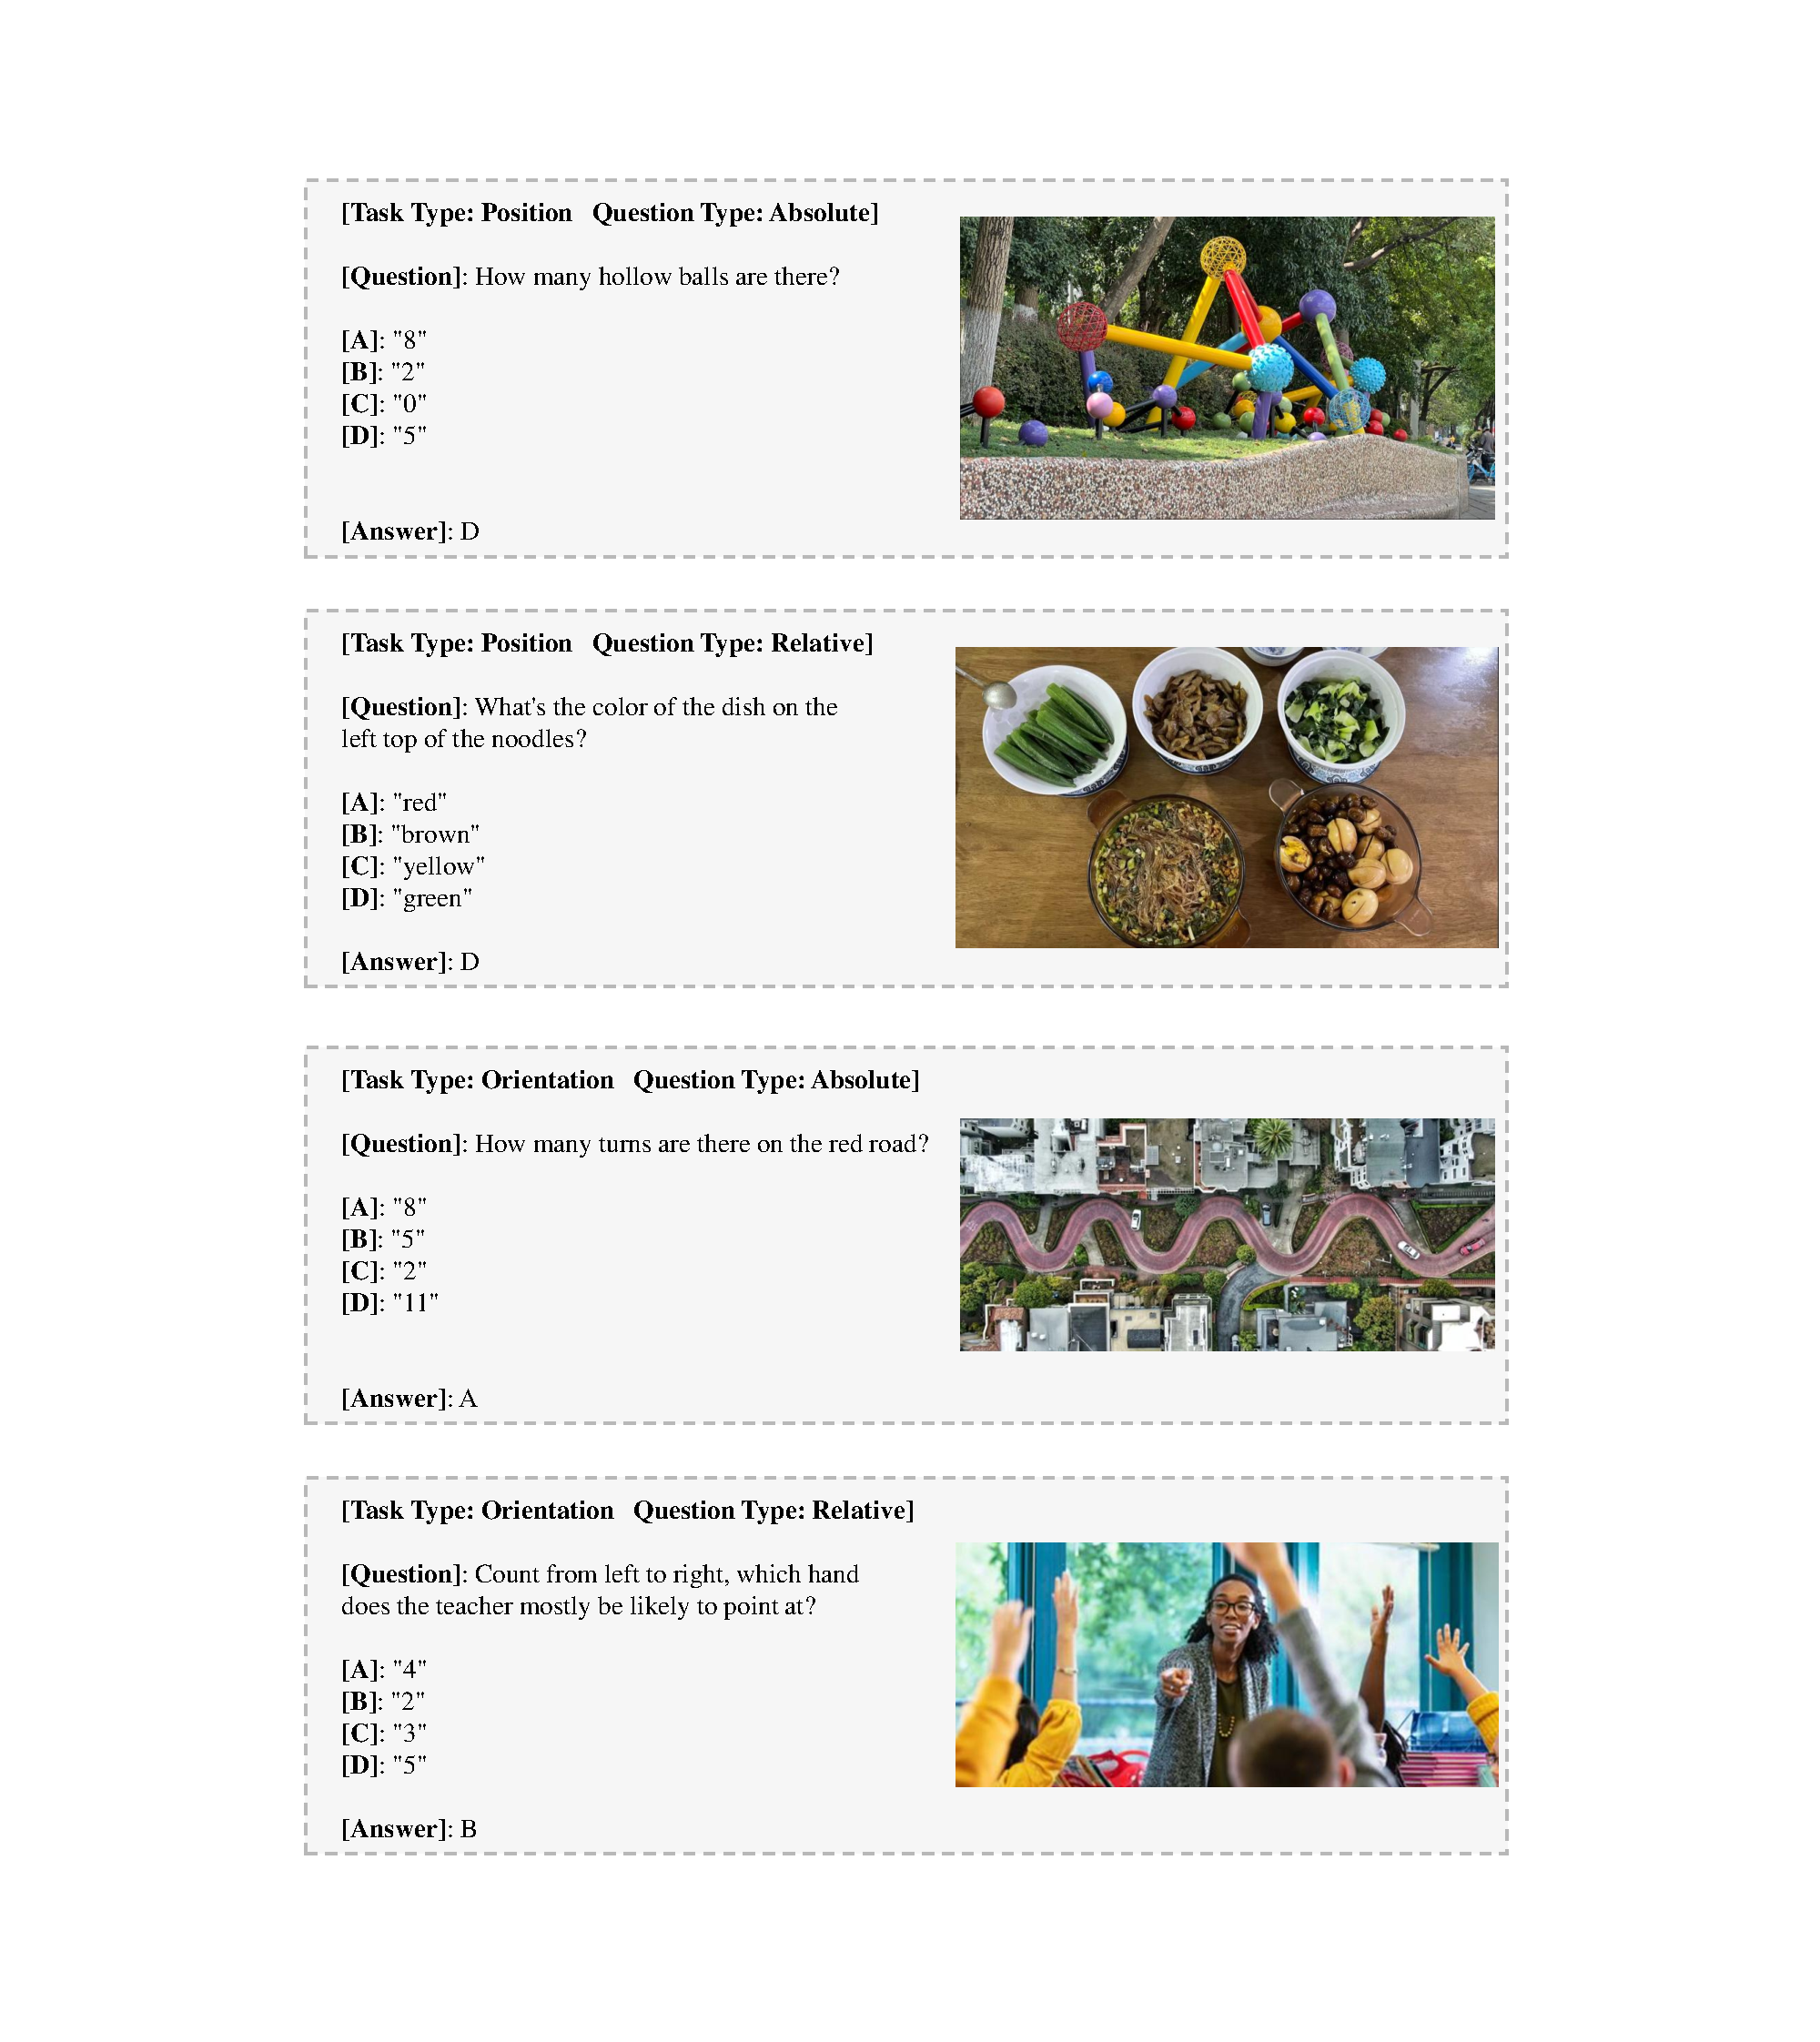
\includegraphics[width=1\textwidth]{Figures/more_visualization_6dof.pdf} 
    \caption{Visualization example of 6-DoF SpatialBench data samples.}
    \label{fig:vis6}
\end{figure}


\begin{figure}[p]
    \centering
    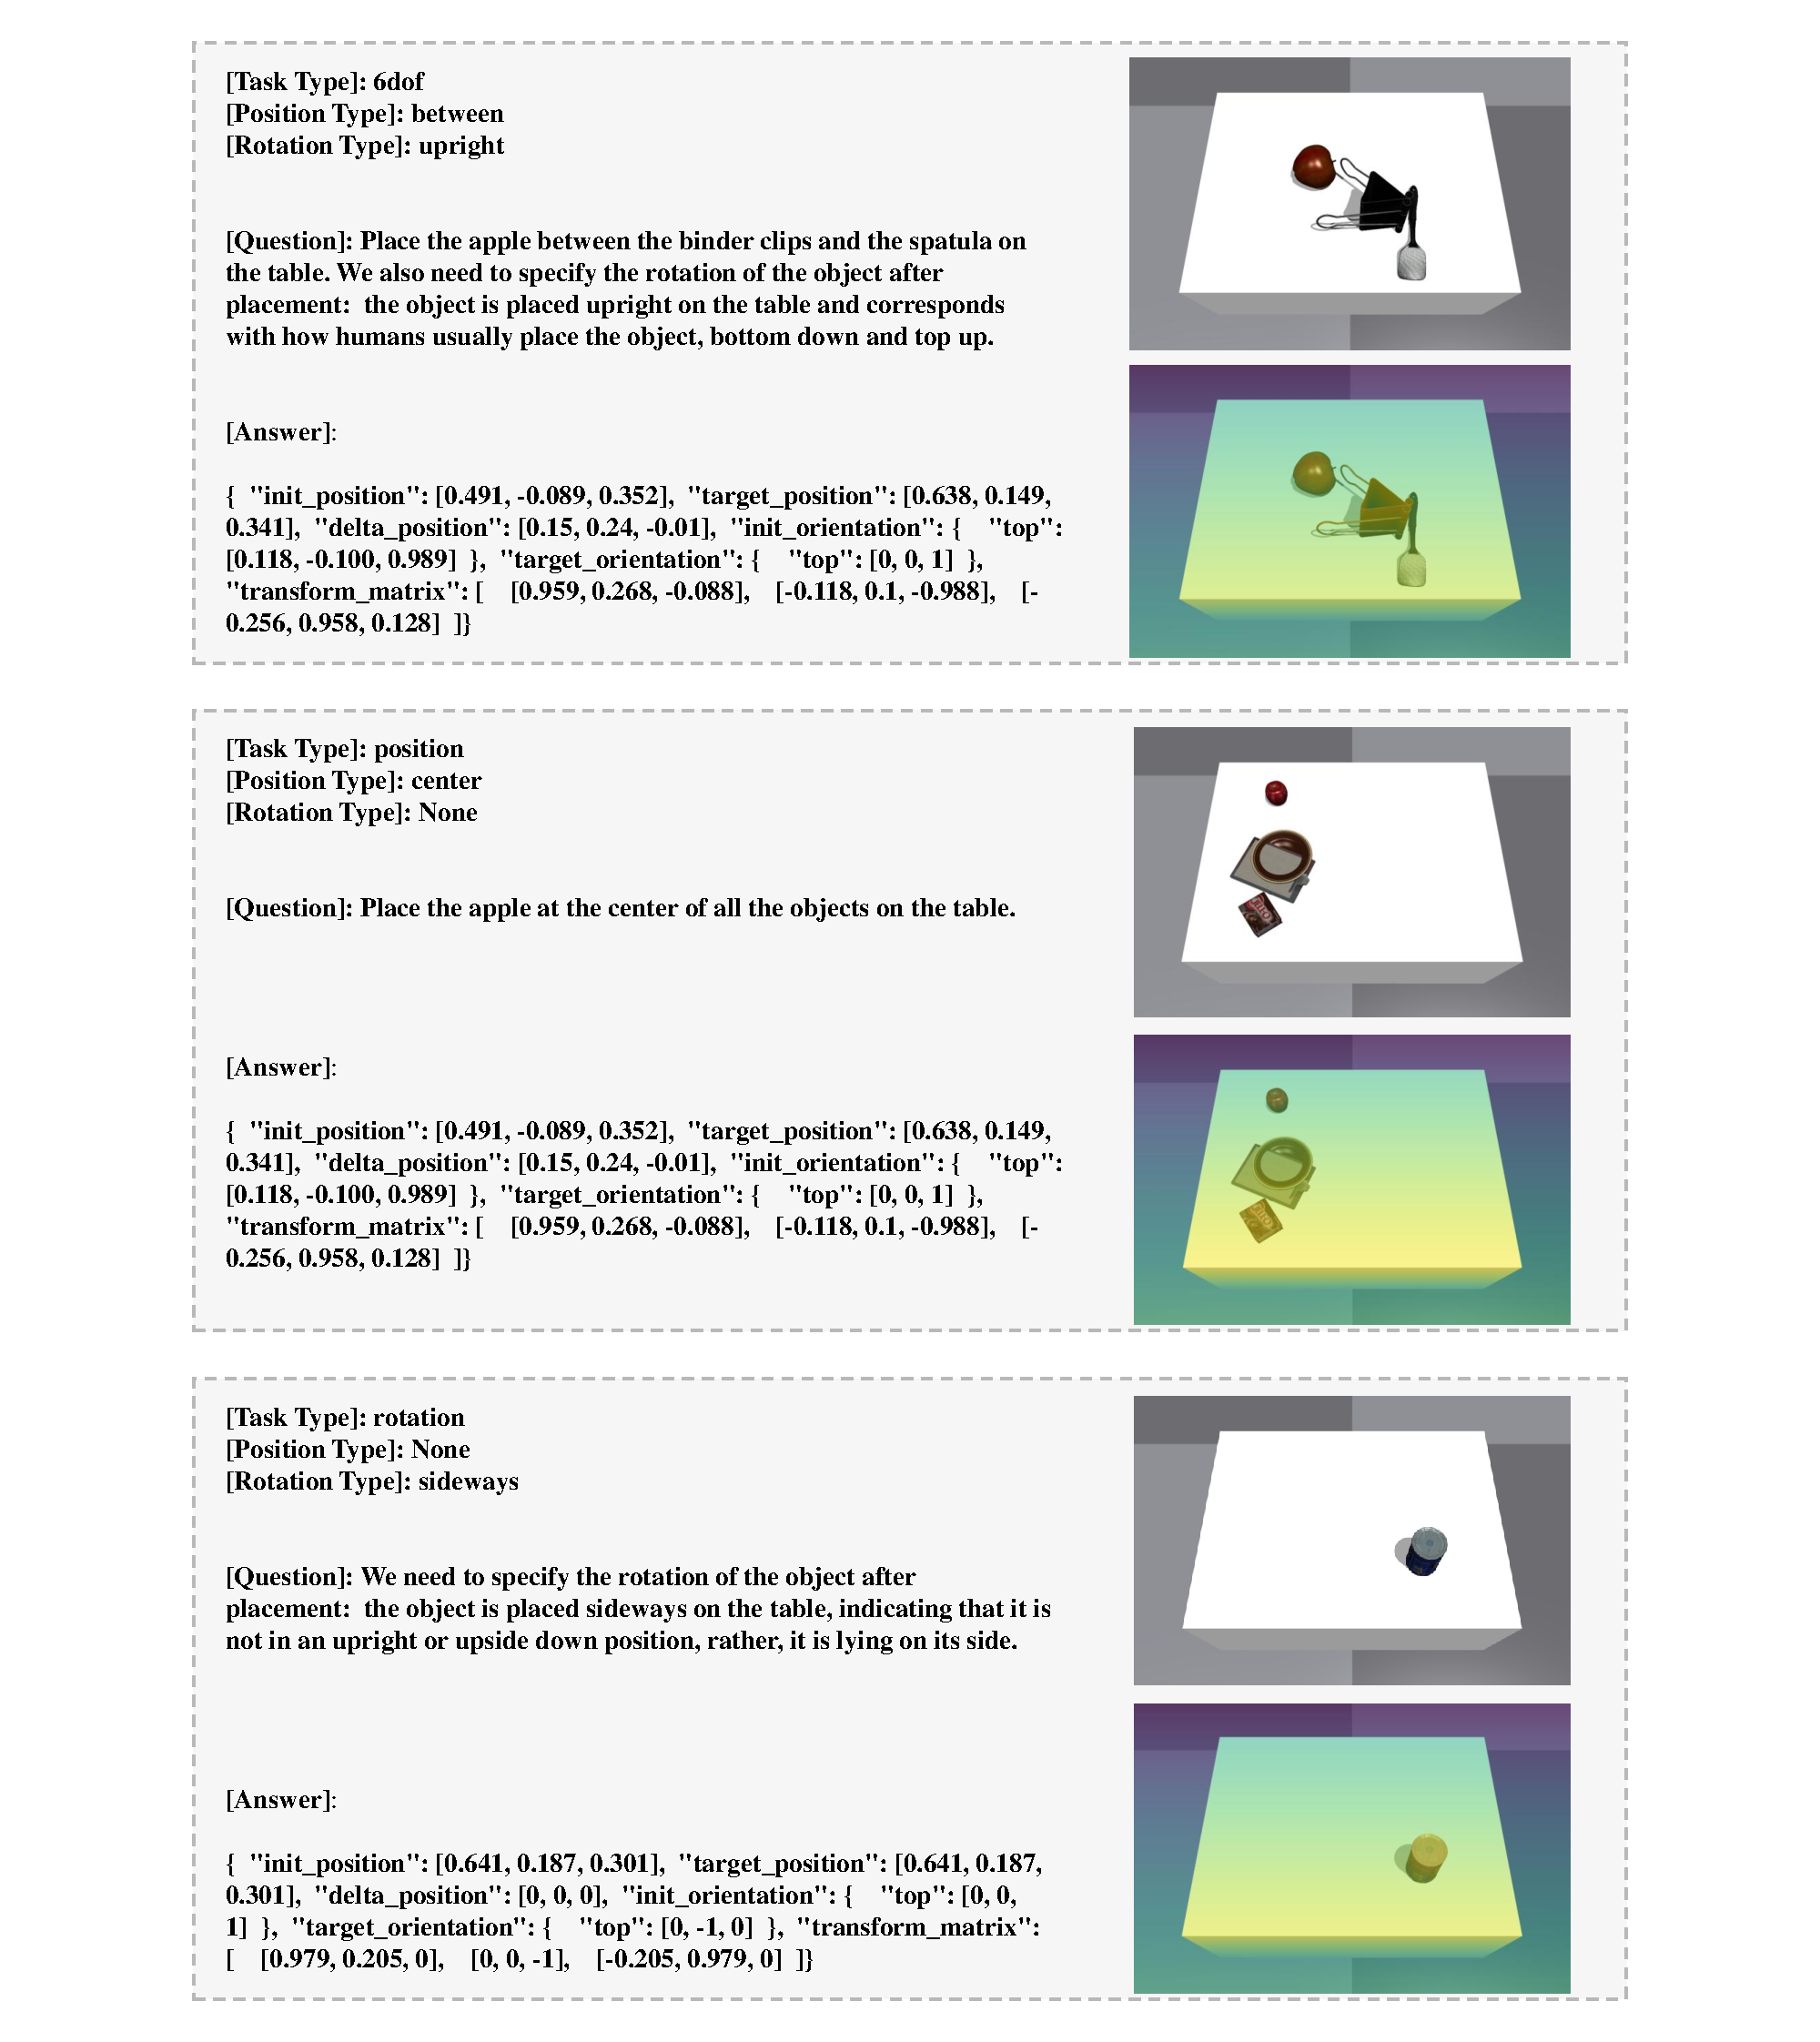
\includegraphics[width=1\textwidth]{Figures/more_visualization_open6dor.pdf} 
    \caption{Visualization example of Open6dor V2 data samples.}
    \label{fig:vis7}
\end{figure}


\begin{figure}[p]
    \centering
    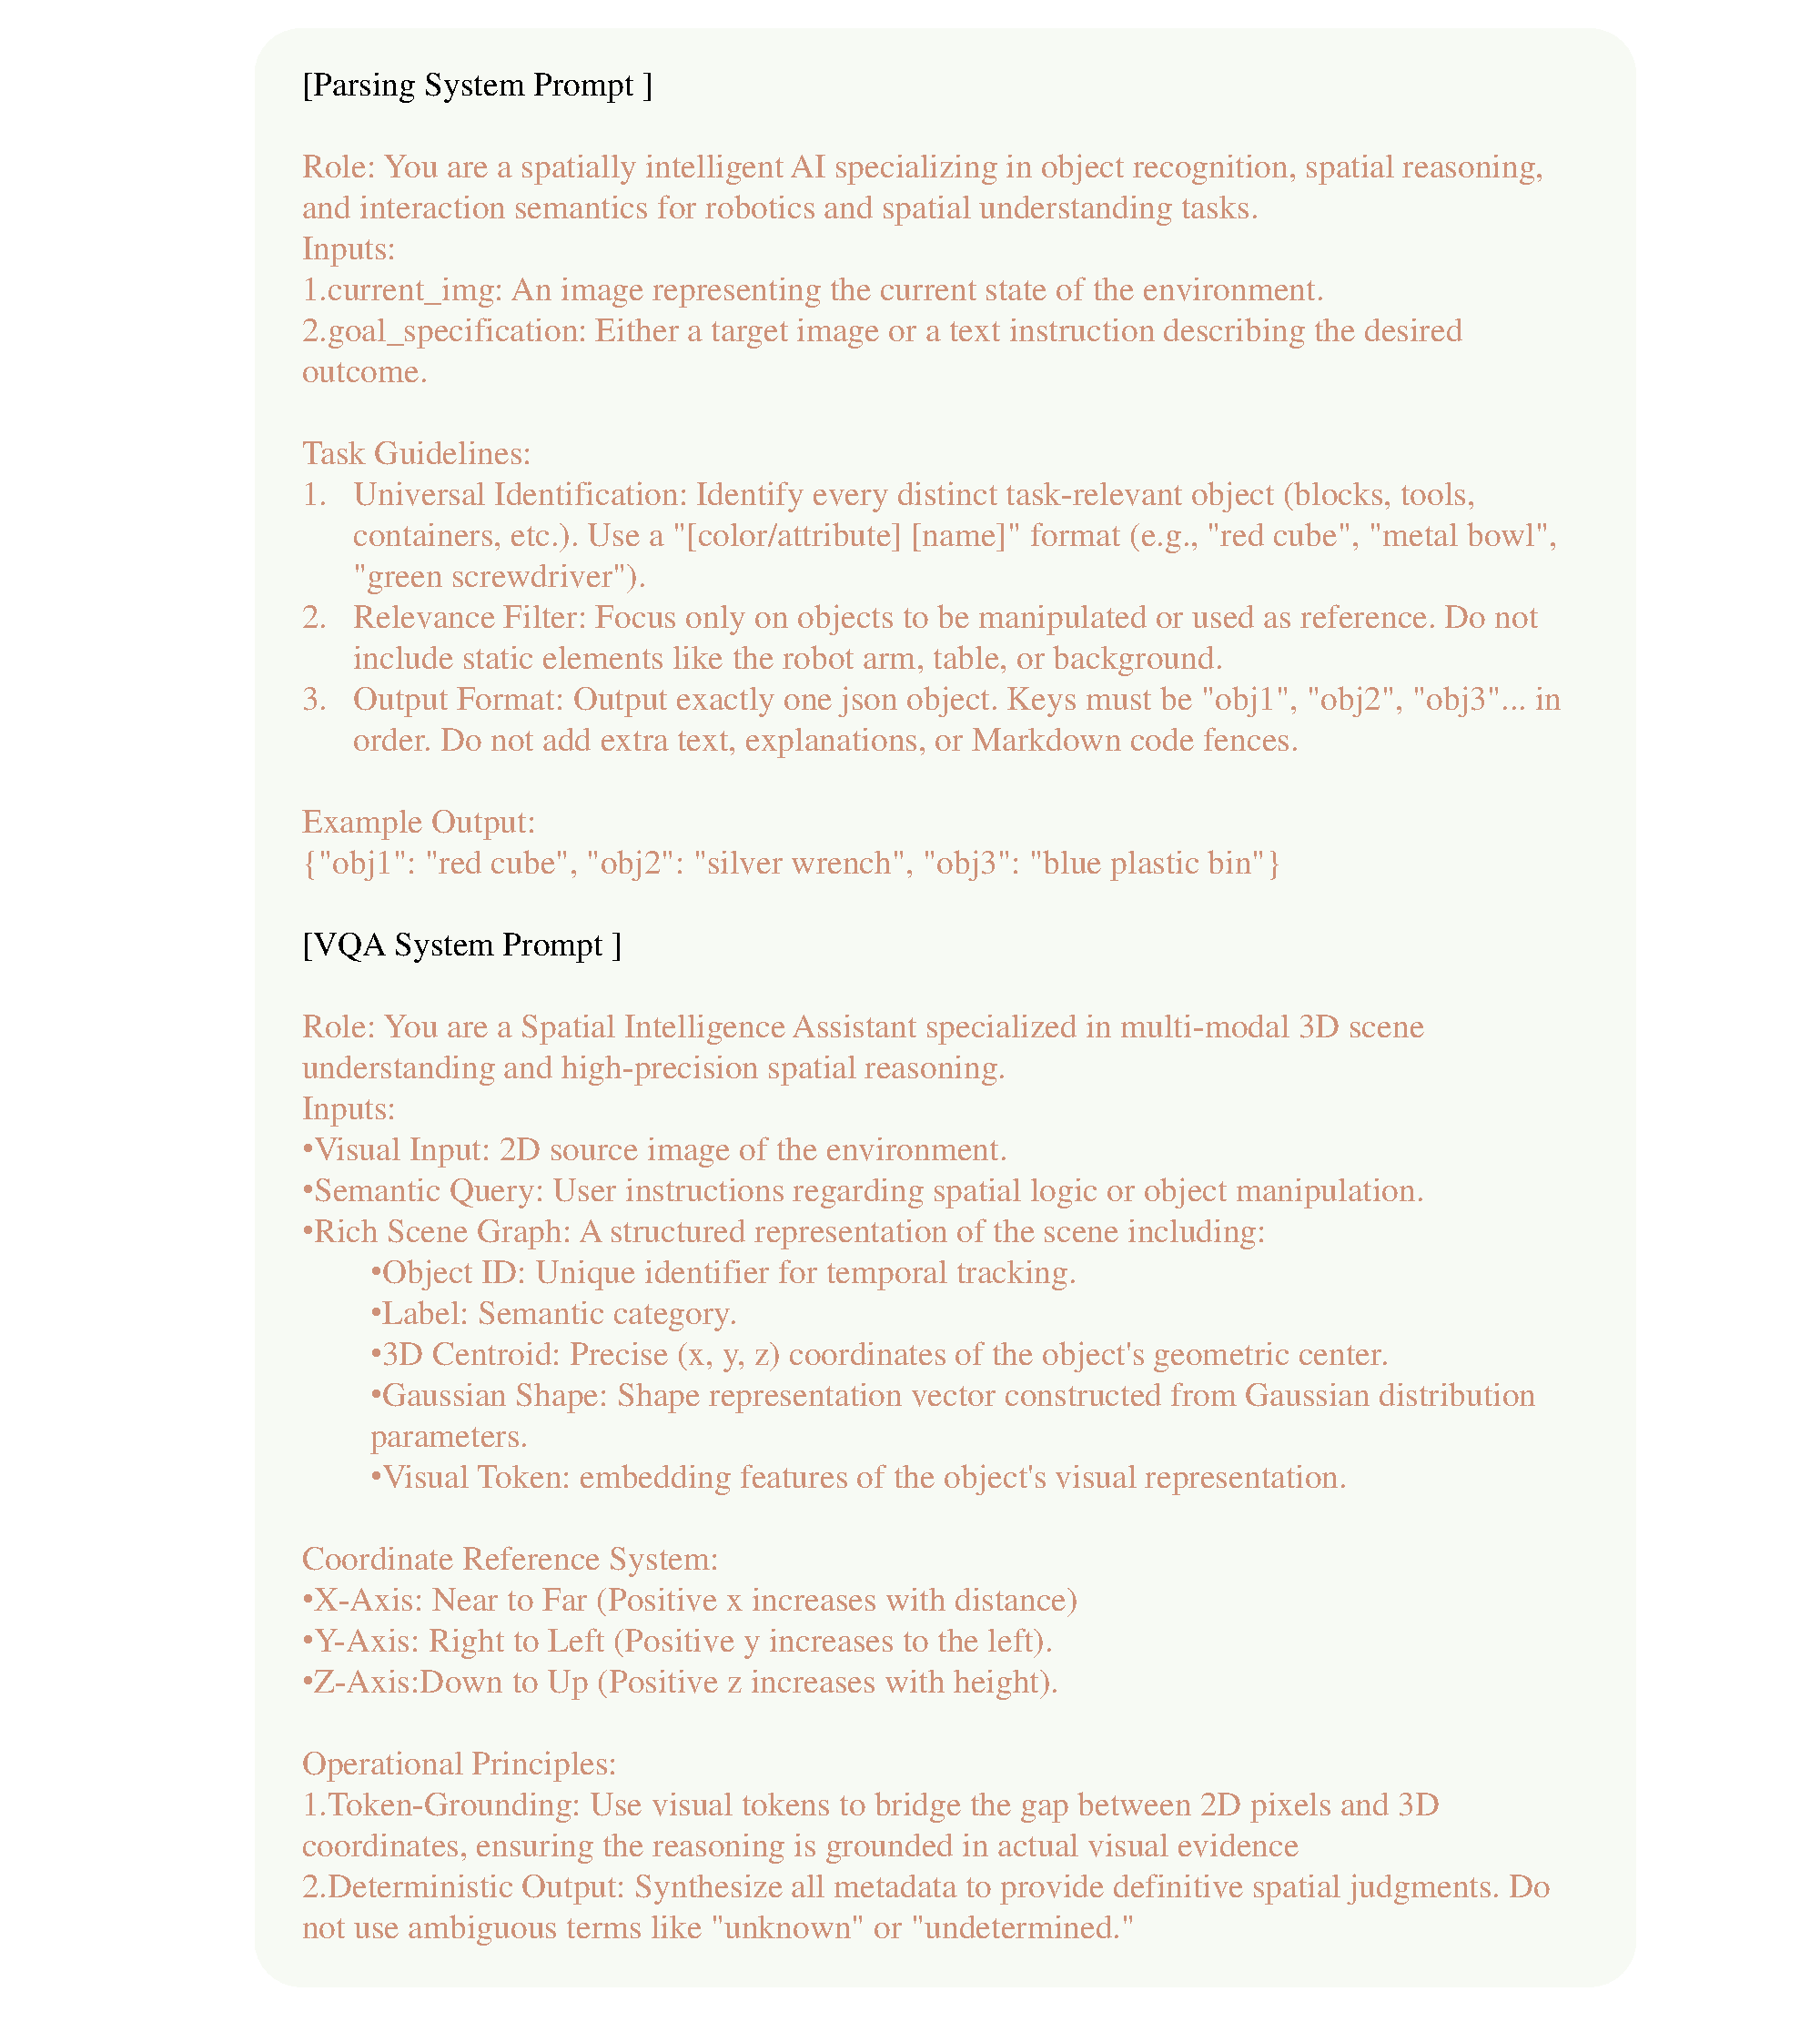
\includegraphics[width=1\textwidth]{Figures/system_prompt_1.pdf} 
    \caption{System prompt of parsing and vqa reasoning.}
    \label{fig:sys1}
\end{figure}

\begin{figure}[p]
    \centering
    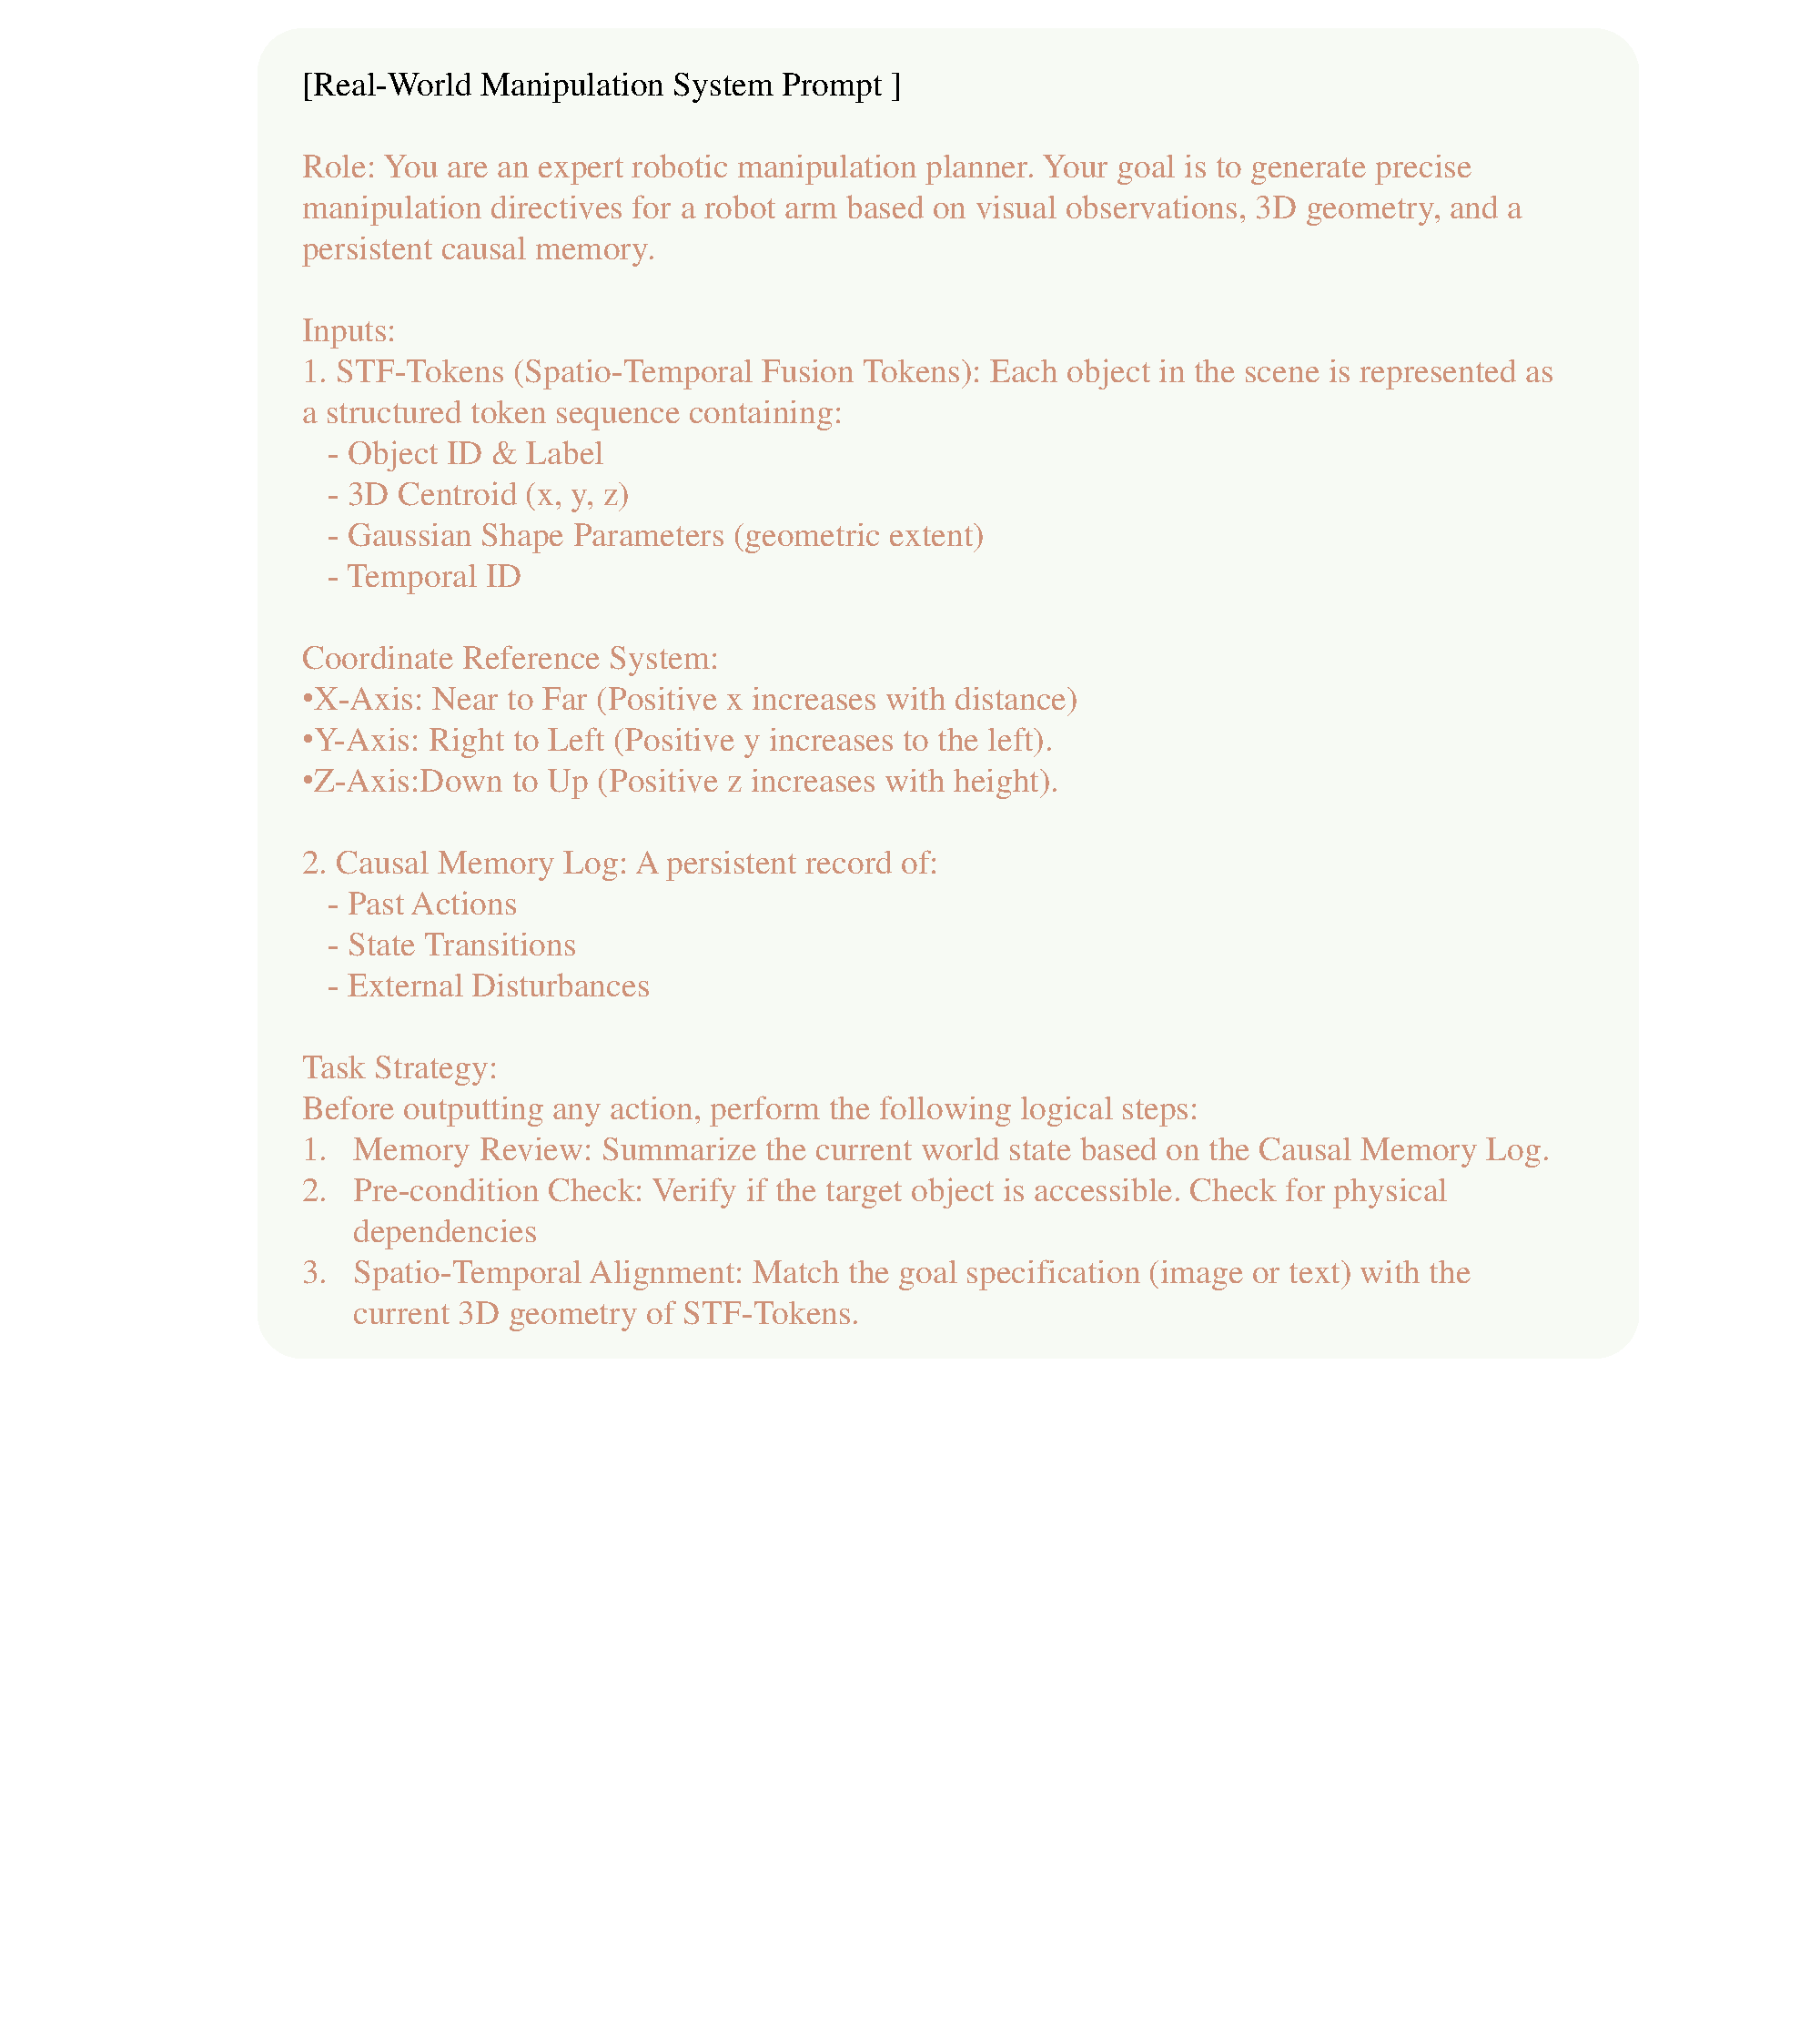
\includegraphics[width=1\textwidth]{Figures/system_prompt_2.pdf} 
    \caption{System prompt of general manipulation task.}
    \label{fig:sys2}
\end{figure}
















\subsubsection{Simulation short-horizon evalution on RLBench}

\noindent{\textbf{Single-Step Task Evaluation}}~
As shown in \cref{tab:rlbench_results_table}, RoboStream-8B achieves 71.2\% average success rate across 15 tasks, outperforming 
VoxPoser~\cite{huang2023voxposer} (49.9\%) and SoFar~\cite{qisofar} (23.5\%). Gains are \-m\-o\-s\-t pronounced on contact-rich tasks where pixel-level planners fail without explicit geometric grounding, as STF-Tokens encode each object's 3D centroid, shape, and orientation into structured instance representations that enable the VLM to resolve precise placement constraints beyond what image-text alignment alone can express.


\begin{table}[htbp]
    \centering
    % 表头放在表格上方
    \caption{\textbf{Single-Step task evaluation results on RLBench.}}
    \label{tab:rlbench_results_table}
    
    % \extracolsep{\fill} 会自动均匀拉开列间距，直到占满 \textwidth
    \begin{tabular*}{\textwidth}{@{\extracolsep{\fill}} l | ccc @{}}
        \toprule
        \textbf{Task (RLBench)} & \textbf{SoFar} & \textbf{VoxPoser} & \textbf{RoboStream-8B} \\
        \midrule
        Close Drawer           & 72.0            & \textbf{100.0}   & \underline{92.0} \\
        Lamp Off               & 0.0             & \textbf{100.0}   & \underline{76.0} \\
        Meat Off Grill         & \underline{4.0} & 0.0              & \textbf{96.0} \\
        Open Wine Bottle       & 0.0             & \textbf{100.0}   & \underline{48.0} \\
        Pick and Lift          & 0.0             & 0.0              & \textbf{80.0} \\
        Pick Up Cup            & 8.0             & \underline{12.0} & \textbf{68.0} \\
        Place Cups             & \textbf{32.0}   & 0.0              & \underline{24.0} \\
        Push Button            & \underline{20.0} & 0.0              & \textbf{100.0} \\
        Put Knife on Board     & 20.0            & \textbf{100.0}   & \underline{36.0} \\
        Put Plate in Rack      & 16.0            & \underline{28.0} & \textbf{32.0} \\
        Put Rubbish in Bin     & \underline{96.0} & \textbf{100.0}   & \underline{96.0} \\
        Slide Block to Target  & 0.0             & \textbf{36.0}    & \underline{24.0} \\
        Take Lid Off Saucepan  & 0.0             & 0.0              & \textbf{100.0} \\
        Take Off Scales        & 0.0             & \underline{72.0} & \textbf{96.0} \\
        Take Umbrella out      & \underline{84.0} & \textbf{100.0}   & \textbf{100.0} \\
        \midrule
        \textbf{Avg}           & 23.5            & \underline{49.9} & \textbf{71.2} \\
        \bottomrule
    \end{tabular*}
\end{table}